\documentclass[a4paper,twoside=true,12pt,openright]{scrbook}
\usepackage{a4}
\usepackage[english]{babel}
\setlength{\parindent}{0.35cm}
\pagestyle{headings}
\usepackage{lmodern}
\usepackage{graphicx}
%Multiple picture in one figure
\usepackage{subfig}
\usepackage{listings}
\usepackage{color}
%Zum Zeilen umbrechen in Tabellen
\usepackage{pbox}
% Using Blindtext
\usepackage{blindtext}
%Configuring figures and captions
\usepackage{floatrow}
%Wrap text around figures
\usepackage{wrapfig}
% Including PDF´s
\usepackage{pdfpages}
%Floating-Umgebungen
\usepackage{float}
%Math-Environment
\usepackage{amsmath}
\usepackage{amssymb}
%For better captions (without regged right from standard format)
\usepackage{caption}
\captionsetup{format=plain,font=normal,labelfont=bf,labelsep=colon} 
%Because Physics is cool
\usepackage{physics}
%Better SI-Units
\usepackage{siunitx}
\DeclareSIUnit\century{century}
\DeclareSIUnit\year{yr}
\sisetup{
	per-mode=fraction,
%	fraction-function=\tfrac
}
%Using Appendix
\usepackage[title]{appendix}
%Using URL
\usepackage[hidelinks]{hyperref}
%Using Colored Tables
\usepackage{colortbl}
%Using text-based symbols
\usepackage{textcomp}
\usepackage{gensymb}
% Zeilenabstand 
\usepackage{setspace}
%\singlespacing        %% 1-zeilig (Standard)
\onehalfspacing       %% 1,5-zeilig
%\doublespacing        %% 2-zeilig
%Set indentation
\setlength\parindent{0.75cm} 
\setlength{\parskip}{0em} % no spacing between paragraphs
%(possibly) fancy tables
\usepackage{booktabs}

% New/Renewing Commands
\newcommand{\eV}{\electronvolt}
\newcommand{\keV}{\kilo\electronvolt}
\newcommand{\meV}{\mega\electronvolt}
\newcommand{\gray}{\rowcolor[gray]{.90}}
\newcommand{\degr}{^{\circ}}
\newcommand{\tit}[1]{\textit{#1}}
\newcommand{\baf}{BaF$_2$}
\newcommand{\pwo}{PbWO$_4$}
\newcommand{\ten}[1]{$10^{#1}$}
\newcommand{\orb}[2]{$#1^{#2}$}
\newcommand{\stat}[2]{$#1_{#2}$}
\newcommand{\ft}[2]{$#1\rightarrow#2$}
\newcommand{\sr}{$^{90}$Sr}
\newcommand{\co}{$^{60}$Co}
\newcommand{\eu}{$^{152}$Eu}
\newcommand{\cs}{$^{137}$Cs}
\newcommand{\ba}{$^{133}$Ba}
\newcommand{\na}{$^{22}$Na}
\newcommand{\ka}{$^{40}$Ka}
%Configure geometry
\usepackage{geometry}
\geometry{
	a4paper,
	left=3cm,
	right=3cm,
	top=3cm,
	bottom = 3cm,
	}

\lstset{
	language=C++,
	basicstyle=\small\ttfamily,
	keywordstyle=\color{blue}\ttfamily,
	stringstyle=\color{red}\ttfamily,
	commentstyle=\color{green}\ttfamily,
	morecomment=[l][\color{magenta}]{\#},
}
\newcommand{\LMUTitle}[9]{
	\thispagestyle{empty}
	\vspace*{\stretch{1}}
	{\parindent0cm
		\rule{\linewidth}{.7ex}}
	\begin{center}
		
		\vspace*{\stretch{1}}
		\sffamily\bfseries\Large
		#1\\
		\vspace*{\stretch{1}}
		\sffamily\bfseries\large
		#2
		\vspace*{\stretch{1}}
	\end{center}
	\rule{\linewidth}{.7ex}
	\vspace*{\stretch{5}}
	\begin{center}
		
\includegraphics[width=2.5in]{logo.jpg}
	\end{center}
	\vspace*{\stretch{1}}
	\begin{center}\sffamily\LARGE{#5}\end{center}
	\newpage
	\thispagestyle{empty}
	
	\cleardoublepage
	\thispagestyle{empty}
	
	\vspace*{\stretch{1}}
	{\parindent0cm
		\rule{\linewidth}{.7ex}}
	\begin{center}
		\vspace*{\stretch{1}}
		\sffamily\bfseries\Large
		#1\\
		\vspace*{\stretch{1}}
		\sffamily\bfseries\large
		#2
		\vspace*{\stretch{1}}
	\end{center}
	\rule{\linewidth}{.7ex}
	
	\vspace*{\stretch{3}}
	\begin{center}
		\Large Bachelor Thesis\\
		\Large am #4\\
		\Large der Justus-Liebig-Universit\"at\\
		\Large Gie\ss{}en\\
		\vspace*{\stretch{1}}
		\Large vorgelegt von\\
		\Large #2\\
		\Large aus #3\\
		\vspace*{\stretch{2}}
		\Large Gie\ss{}en, den #6
	\end{center}
	
	\newpage
	\thispagestyle{empty}
	
	\vspace*{\stretch{1}}
	
	\begin{flushleft}
		\large Betreuer: #7 \\[1mm]
		\large Erstgutachter:  #8 \\[1mm]
		\large Zweitgutachter: #9 \\[1mm]
		\large Tag der Abgabe: #6\\
	\end{flushleft}
	
	\clearpage
}

\begin{document}


\LMUTitle
	{Aufbau und Test eines SiPM-basierten Auslesemoduls zur Charakterisierung von Szintillationsmaterialien \\ $-$ \\ 
	Development of a SiPM-based readout-module for the characterization of various scintillator materials }               % Titel der Arbeit
	{Lukas Nies }                       % Vor- und Nachname des Autors
	{Nidda}                             % Wohnort des Autors
	{II. Physikalischen Institut}                         % Name der Fakultaet
	{Gie\ss{}en, 2017}                          % Ort und Jahr der Erstellung
	{17. August 2017}                            % Tag der Abgabe
	{Prof. Dr. Kai-Thomas Brinkmann}
	{Prof. Dr. Kai-Thomas Brinkmann}                          % Name des Erstgutachters
	{PD Dr. Jens S{\"o}ren Lange AR }                         % Name des Zweitgutachters

\cleardoublepage

\frontmatter

\chapter*{Abstract}
\addcontentsline{toc}{chapter}{Abstract}%

Modern photodetector applications encounter a large spectrum of different experimental environments. Prerequisites like working within strong magnetic fields, providing large intrinsic amplification, no dependence on high operation voltage, and space restrictions lead to the development of a new type of detectors, the semiconductor diodes. The \tit{Silicon Photomultiplier} (SiPM) integrates a huge number of \tit{avalanche photodiodes} as microcells within a small space. With a large intrinsic amplification of up to $10^6$, the SiPM comes in many different packaging sizes and works mainly with low voltage between $\SI{25}{\volt}$ and $\SI{85}{\volt}$. Its insensitivity to magnetic fields and single photon counting capability in combination with suited scintillators make SiPMs a valuable choice for modern challenging applications, i.e. \tit{nuclear magnetic resonance imaging} or \tit{positron emission tomography}. \par 
In this thesis, the first three chapters cover the theoretical foundation, i.e. particle interaction with matter, scintillators and semiconductor photodiodes. In the fourth chapter, the development, characterization, and application of a SiPM-based readout-module will be depicted. This includes temperature dependent measurements of IV-characteristics for determining the breakdown voltage and operation voltage with different configurations. In addition, the dark count rate and the dark electron spectrum are measured. The signal readout for raw and amplified solutions will be introduced. Furthermore, the fifth chapter will cover the measurement of efficiency and timing resolution properties in combination with a plastic scintillator, \tit{EJ-248M} from \tit{ELJEN}, in which the propagation time of photons in matter will be examined. In closing, the energy resolution for two prominent inorganic scintillators, LYSO and \pwo{}, will be tested by taking energy spectra with various calibration sources. The last part of this thesis will present a measurement of the energy loss of cosmic muons in lead tungstate.  

\chapter*{Zusammenfassung}
\addcontentsline{toc}{chapter}{Zusammenfassung}%

Weitreichende Anforderungen stellen Photodetektoren in modernen Anwendungen vor immer neue Herausforderungen. Einschr{\"a}nkungen wie das Funktionieren in starken magnetischen Feldern, eine gro\ss e intrinsische Verst{\"a}rkung, Niedrigspannungsversorgung und Handlichkeit f{\"u}rten zur Entwicklung einer neuen Art von Detektoren, den Halbleiterdioden. Der Siliziumphotovervielfacher (SiPM) integriert eine gro\ss e Menge an Lawinenphotodioden (APD) als Mikrozellen auf kleinem Raum. Mit einer gro\ss en intrinsischen Ver{\"a}rkung von bis zu $10^{6}$ werden SiPMs in vielen verschiedenen Gr{\"o}\ss en hergestellt und werden haupts{\"a}chlich mit Niedrigspannung, typisch zwischen $\SI{25}{\volt}$ und $\SI{85}{\volt}$, betrieben. Die Unempfindlichkeit gegen{\"u}ber magnetischen Feldern und die F{\"a}higkeit, einzelne Photonen z{\"a}hlen zu k{\"o}nnen, machen die SiPM in Kombination mit einem geeignetem Szintillator zu einer exzellenten Wahl, um in anspruchsvollen Anwendungen, wie zum Beispiel die Magnetresonanz-Thomographie oder die Positron-Emissions-Thomographie, eingesetzt zu werden. \par
In den ersten drei Kapiteln dieser Thesis werden die Grundlagen dieser Arbeit behandelt, die Wechselwirkung von Teilchen mit Materie, Szintillatoren und Halbleiter-Photodetektoren. Im vierte Kapitel wird die Entwicklung, Charakterisierung und Anwendung eines SiPM-basierten Auslesemoduls vorgestellt. Unter anderem wird die Tem\-pe\-ra\-tur\-ab\-h{\"a}n\-gig\-keit der Strom-Spannungscharakteristik f{\"u}r verschiedene Konfigurationen untersucht, um aus diesen die Durchbruchspannung und optimale Betriebsspannung zu erlangen. Zus{\"a}tzlich werden die Dun\-kel\-z{\"a}hl\-ra\-ten und Dunkelspektren gemessen, sowie die Auslese von Roh- und verst{\"a}rkten Signalen vorgestellt. Im f{\"u}nften kapitel wird die Effizienz und Zeitaufl{\"o}sung in Verbindung mit einem Plastikszintillator, \tit{EJ-248M} von \tit{ELJEN}, untersucht, indem die Laufzeiten von Photonem im Szintillatormaterial gemessen werden. Zus{\"a}tzlich wird die E\-ner\-gie\-auf\-l{\"o}\-sung in Verbindung mit zwei inorganischen Szintillatoren, LYSO und \pwo{} getestet. Als Abschluss wird das Energieverlust-Spektrum von kosmischen Myonen in Bleiwolframat aufgenommen.


















\clearpage

\chapter*{Danksagungen\\ \LARGE \normalfont Acknowledegments}
\addcontentsline{toc}{chapter}{Acknowledgements}%

An dieser Stelle m{\"o}chte Ich mich zuerst bei meiner Familie bedanken, die mir das Studieren erm{\"o}glicht und mich in allen Lebenslagen unterst{\"u}tzt. Besonders bedanke Ich mich bei meine Bruder Jonas, der diese Thesis Korrektur gelesen hat. \par 
Danke auch an alle Kommilitonen und Freunde, die mich w{\"a}hrend des Bachelorstudiums begleitet haben und die mich bei mancher langweiligen Zugfahrt oder eint{\"o}nigen Vorlesung abgelenkt und unterhalten haben. \par 
Ganz besonders bedanke ich mich bei Herrn Prof. Kai-Thomas Brinkmann, der mir die M{\"o}glichkeit gab, nicht nur die Bachelorthesis in seiner Arbeitsgruppe schreiben zu k{\"o}nnen, sondern auch seit {\"u}ber eineinhalb Jahren Gelegenheit gibt, in der Arbeitsgruppe an interessanten Themen mitzuarbeiten. Mein Dank gilt hier ebenfalls Herrn Dr. S{\"o}ren Lange, der diese Thesis als Zweitgutachter bewertet. \par
Des Weiteren bedanke ich mich bei allen Mitgliedern der Arbeitsgruppe und allen Mitarbeitern der Elektronikwerkstatt des II. Physikalischen Institutes, die mir in den letzten Monaten mit Rat und Tat zu Seite standen, besonders bei Herrn Ren\'{e} Schubert, der immer mit gr{\"o}\ss ter Fachkenntnis zur Stelle war, wenn es technische Probleme zu beheben gab. Weiterer Dank gilt Herrn Dr. Eric Gutz, der mich bei Formalit{\"a}ten beraten und beim Schreibprozess begleitet, sowie einige Stunden des Korrekturlesens der Thesis investiert hat. F{\"u}r seine Fachkenntnisse, Hilfe und Rat bei der Durchf{\"u}hrung und Auswertung der Experimente und weit dar{\"u}ber hinaus bedanke ich mich ganz besonders bei Herrn Dr. Hans-Georg Zaunick, der mich schon seit Beginn meiner Arbeit in der Arbeitsgruppe motiviert und unterst{\"u}tzt. \par 
Abschlie\ss end bedanke ich mich bei meinem Freund und Kommilitonen Wihan Adi, mit dem das Forschen und Schreiben der Arbeit deutlich einfacher und entspannter von Hand ging, sowie bei Christopher Hahn und Benjamin Wohlfahrt, die mich und Wihan freundlich in Ihrem B{\"u}ro aufgenommen und uns ``ertragen" haben. \par 
Nochmals vielen Dank an Alle!






\clearpage

\thispagestyle{empty}
\tableofcontents
\cleardoublepage
\mbox{}
\thispagestyle{empty}
\newpage
\newpage
\setcounter{page}{0}

\mainmatter

% !TEX root = Nies_Lukas_BSc_Thesis_SiPM.tex

\chapter{Particle interaction with matter} \label{ch:particles}

As numerous kinds of particles exist as diverse are their types of interaction with matter. To classify this, one not only has to consider the particles' mass, charge and energy but also their behavior due to interaction through the fundamental forces. To describe some of the most essential interactions, a brief overview is given in the following.      

\section{Interaction of photons}

The photon is a neutral and massless particle. As the force carrier of the electromagnetic force the photon interacts electromagnetically. Since photons have no mass they always move with the speed of light. Their energy is given by the product of the Planck constant $h$ and the frequency $\nu$
\begin{align}
E=h\cdot\nu=h\cdot\frac{c}{\lambda},
\end{align}
where $\lambda$ is the corresponding wavelength. The interaction of these particles depends on their energy, the different types are shown in figure \ref{fig:ch1:photons}.\par 
Photons with low energy (long wavelength) do elastic scattering with electrons (\textit{compton scattering}). In this process they are deflected by an angle $\vartheta$ and lose energy, $E_{\gamma}'$, to the electron. This mechanism leads to an increase of wavelength 
\begin{align}
\Delta\lambda=\frac{h}{m_ec}\left(1-\cos(\vartheta)\right)=\lambda_c\left(1-\cos(\vartheta)\right) \label{eq:compton_wavelength},
\end{align}
where $m_e$ is the mass of an electron and $\lambda_c$ is the so called \textit{compton wavelength}. It can be seen that the energy deposit at $\vartheta=180\degree$ is largest. The energy gain of the electron is given by 
\begin{align}
E_e'=E_\gamma-E_\gamma'=E_\gamma\left(1-\frac{1}{1+\frac{E_\gamma}{m_ec^2}\left(1-\cos(\vartheta)\right)}
\right).
\end{align} \\[0.5cm] 
\par 
\begin{figure}[t]
	\floatbox[{\capbeside\thisfloatsetup{capbesideposition={left,center},capbesidewidth=5cm}}]{figure}[\FBwidth]
	{\caption[Interaction of phtonos with matter]{Energy dependency of the attenuation coefficient $\mu/\rho\sim\sigma$ in lead \cite{povh}. The cross section rises suddenly when the photon-energy is high enough to excite an inner shell. A more detailed version can be found in figure \ref{ap:A:photons_detailed}.}    
	\label{fig:ch1:photons}}
	{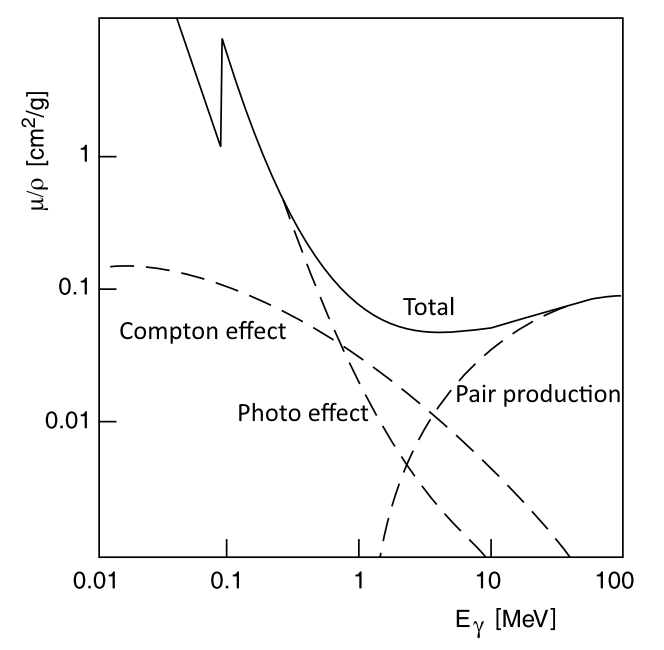
\includegraphics[width=0.6\textwidth]{./graphics/ch1/photo_absorption.png}}
\end{figure}
When it comes to higher energies the \textit{photoelectric effect} comes into play. It describes the entire absorption of a photon by an atomic shell where the absolute photon-energy $E_\gamma$ is transferred to an electron with binding energy $E_B$
\begin{align*}
h\nu + \text{atom} = \text{atom}^{+}+e^{-}.
\end{align*} 
The electron gets unbound when $E_\gamma>E_B$ and the atom gains momentum through the recoil which is small due to its high mass. For higher energies, electrons from inner shells (K,L,M,...) can be removed, too. This mechanism is favored since the cross section for these processes is high when $E_\gamma-E_B$ is low \cite{wermes}. This generates a higher cross section for inner shells which is visualized by a sudden rise in figure \ref{fig:ch1:photons}.\par 
\textit{Pair production} is possible when the photon energy exceeds twice the electrons' invariant mass ( $E_\gamma\gtrsim 2m_ec^2\approx\SI{1.02}{\MeV}$ ): the photon converts into an electron-positron-pair in an external electromagnetic field. As before, the recoil energy can be neglected. This process is dominating for very high energies.\par 
All these mechanisms lead to a scattering or an absorption of photons. This loss of particles is described by \textit{Beer-Lambert's Law}
\begin{align}
N(x)&=N_0e^{-\mu x}=N_0e^{-\frac{x}{\lambda}}, 
\label{eq:beer_lambert}
\end{align} 
where $N_0$ is the initial number of particles in a photon beam, $\mu$ the attenuation coefficient and $\lambda$ the mean free path between collisions. The formula can be derived by shifting and integrating the definition of the attenuation coefficient which illustrates the ability of a material to absorb photons:
\begin{align}
\mu=-\frac{1}{N}\dv{N}{x}=\rho\frac{N_A}{A}\sigma=n\sigma=\frac{1}{\lambda}.
\end{align}
It can be seen that the absorption of photons depends on the materials' density $\rho$ and mass number $A$, $N_A$ is the \textit{Avogadro number}. 

\section{Interaction of charged particles}

A heavy charged particle interacting with matter loses energy through excitation and ionizing processes. These \text{ionization losses} can be expressed by the \textit{Bethe-Bloch formula}, which gives the \textit{stopping power} $S=-\dv{E}{x}$ of particles in matter: 
\begin{align}
-\langle\dv{E}{x}\rangle=\frac{4\pi}{m_ec^2}\frac{nz^2}{\beta^2}\left(\frac{e^2}{4\pi\epsilon_0}\right)^2\left[\ln\frac{2m_ec^2\beta^2}{I\cdot(1-\beta^2)}-\beta^2\right].
\label{eq:bethe_bloch}
\end{align}
\begin{center}
	\centering
	\small
	$ze$ and $\beta=\frac{v}{c}$: charge and velocity of incident particle, $I$ and $n$: mean ionization potential and electron density of the matter 
\end{center}
This equation approximates the mean energy loss d$E$ per length d$x$ in an area of $0.1<\beta\gamma<1000$ \cite{PDG}. This correlation is shown in figure \ref{fig:ch1:bethe_bloch}. The energy loss for small momenta is large since the interaction time is longer for slow particles. The graph decreases with $1/\beta^2$ for greater energies and reaches a minimum at approximately $\beta\gamma=3-4$. At this point the so called \textit{minimum ionizing particles (MIP)} dissipate roughly 2 $\si{\MeV\per\gram\per\square\centi\meter}$. A relativistic rise with almost $\sim\ln(\gamma)$ follows for growing $\beta\gamma$ due to rare large energy transfers to few electrons \cite{PDG}. \par 
\begin{figure}[b]
	\floatbox[{\capbeside\thisfloatsetup{capbesideposition={right,center},capbesidewidth=5cm}}]{figure}[\FBwidth]
	{\caption[Interaction of charged particles with matter]{Normalized energy loss of particles in different targets \cite{povh}. The x-axis shows the particle energies in $\beta\gamma=p/mc$. Again, a more detailed version can be found in figure \ref{ap:A:bethe_bloch_detailed}.}    
		\label{fig:ch1:bethe_bloch}}
	{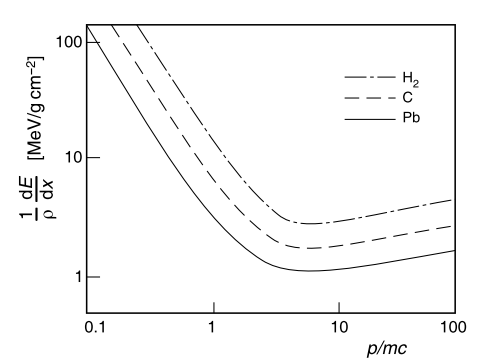
\includegraphics[width=0.6\textwidth]{./graphics/ch1/bethe_bloch.png}}
\end{figure}
Due to their small mass, electrons mainly lose energy by emitting \textit{brems\-strah\-lung} when decelerated in an electromagnetic field of a nucleus. These \textit{radiation losses} depend on the effective nuclear charge $Z_{\text{eff}}^2$ due to shielding effects of bound electrons and the concentration $n$ of electrons in the solid \cite{rodnyi}
\begin{align}
-\dv{E}{x}=Z_{\text{eff}}^2\cdot nE_0, 
\label{eq:energy_loss_electrons}
\end{align}  
where $E_0$ is the energy of the incident electron. \par   
\begin{figure}[t]
	\floatbox[{\capbeside\thisfloatsetup{capbesideposition={left,center},capbesidewidth=5cm}}]{figure}[\FBwidth]
	{\caption[Interaction of electrons with matter]{Energy loss of electrons in silicon. Ionization processes are dominating for low energies. The intersection of the dashed lines gives the critical energy above bremsstrahlung influences most. The dotted curve shows the Bethe-Bloch-like behavior of protons as comparison. Amended from \cite{wermes}.}    
		\label{fig:ch1:electrons}}
	{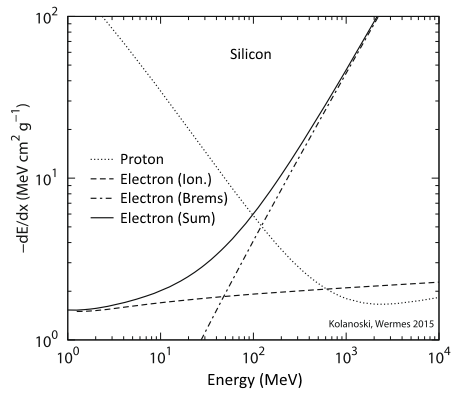
\includegraphics[width=0.6\textwidth]{./graphics/ch1/energy_loss_electrons.png}}
\end{figure}
Ionization losses caused by \tit{coulomb scattering} dominate at lower energies. The \tit{critical energy} gives the energy where radiation losses become the dominant process. It can roughly be estimated by 
\begin{align}
E_c\approx\frac{800}{Z_{\text{eff}}},
\label{eq:radiation_length}
\end{align}
given in $\si{\MeV}$ \cite{rodnyi}. Figure \ref{fig:ch1:electrons} illustrates the energy loss of electrons in silicon, the critical energy is given by the intersection of the dashed lines. A \textit{radiation length} $X_0$ can be formulated analog to $\lambda$ in formula \eqref{eq:beer_lambert}. \par 
Due to bremsstrahlung, incident high energy electrons produce photons with sufficient energy to create electron-positron-pairs. These secondary products have enough energy to produce even more particles. The resulting \textit{electromagnetic shower} only stops when the energy of the cascade electrons falls below the critical energy \cite{rodnyi}. The \textit{Moli\`{e}re radius} can be approximated by
\begin{align}
R_M=\frac{21X_0}{E_c}
\label{eq:moliere} 
\end{align}
and provides an estimation of the transversal geometry of a defocussing, cone-like shower. This relation also applies to high energy photons.        

\section{Interaction of hadrons}
Neglecting the electromagnetic interaction, the interplay of hadrons (p,n,$\pi$,K,...) with matter is hard to calculate since the strong force knows many different interaction processes. To give a short qualitative approach, one can define a \textit{hadronic interaction length}  
\begin{align}
\lambda_a=\frac{A}{N_A\rho\sigma_{\text{in}}}\propto A^{-\frac{2}{3}}
\end{align}
analogous to the relations \eqref{eq:beer_lambert} and \eqref{eq:radiation_length}, where $\rho\sim A$ is the materials' density and $\sigma\sim A^{\frac{2}{3}}$ is the cross section for inelastic scattering \cite{wermes}. \par 
Neutrons as the most prominent uncharged hadron interact via scattering and absorption with nuclei. Inelastic scattering is favored for higher energies ($\sim \SI{10}{\MeV}$). For lower energies, elastic scattering and absorption are likely. Both processes excite the nuclei which then emit a photon. This is important when it comes to moderating hot neutrons to receive cold (low energy) neutrons. 

\chapter{Scintillators} \label{ch:scintillators}
The detection of previously described particles is a key task in various applications like radiation monitoring, research and nuclear medicine. The material class of \tit{scintillators} provides candidates in diverse shapes, densities and phases for numerous requirements. In this chapter, solid scintillators are introduced.
\section{Overview}
The generation of \tit{luminescence}, emission of light with a characteristic spectrum caused by interaction of ionizing particles due to compton scattering, photoeffect and pair production (see chapter \ref{ch:particles}), is called \tit{scintillation}. 
\begin{figure}[b]
	\floatbox[{\capbeside\thisfloatsetup{capbesideposition={right,center},capbesidewidth=6.5cm}}]{figure}[\FBwidth]
	{\caption[Stokes shift]{Stokes shift for emission and absorption \cite{wermes}. The shift must be high enough to avoid re\-absorption and low enough to ideally exploit the absorption capability of the photodetector (see chapter \ref{ch:photo_detectors}).}   
		\label{fig:ch2:stokes}}
	{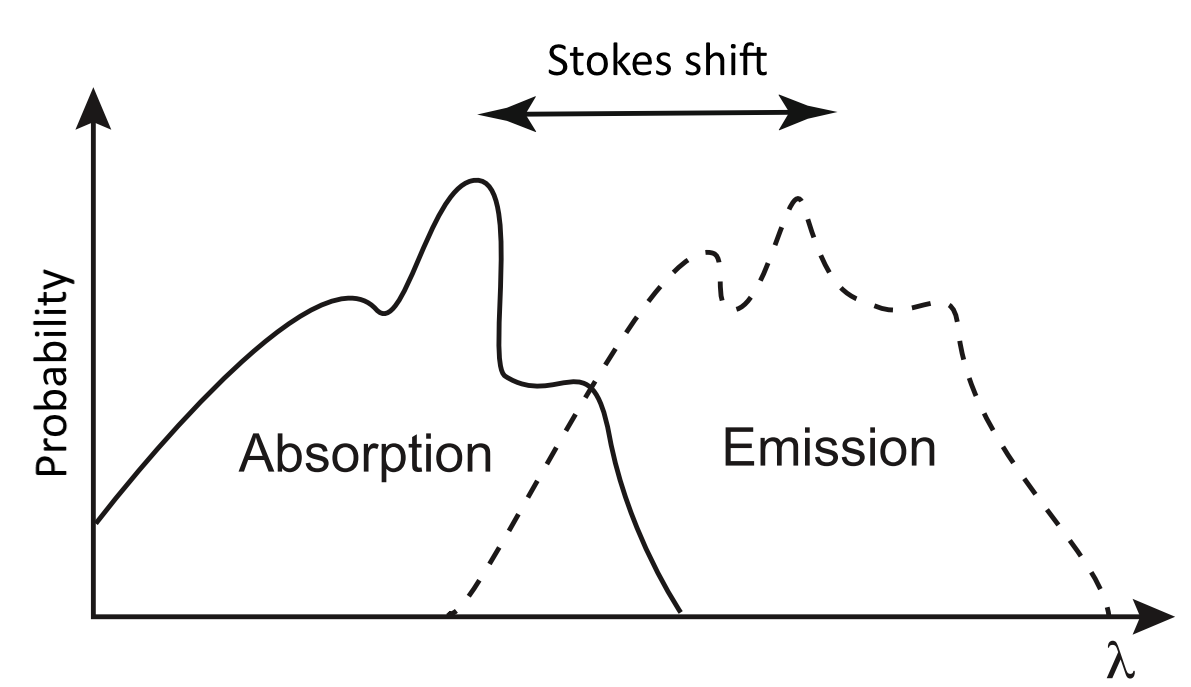
\includegraphics[width=0.5\textwidth]{./graphics/ch2/stokes.png}}
\end{figure}
The excitation, relaxation and recombination processes responsible for the emission of photons are diverse and complex, some of them will be briefly discussed later. An ideal scintillator should provide the following characteristics \cite{wermes}:
\begin{itemize}
	\setlength{\itemsep}{0pt}
	\item High \tit{light yield} (quantity of photons per energy): $L_S=\frac{<N_{ph}>}{E} \label{eq:light_yield}$. Should be proportional to the deposited energy (\tit{linearity}). 
	\item Transparency for emitted light. A high wavelength shift (\tit{Stokes shift}) to higher wavelengths for the emitted photon spectrum compared with the absorption is desired to avoid re\-absorption (see figure \ref{fig:ch2:stokes}).  
	\item Short decay time for fast response and high rates.
	\item High radiation length for full-energy measurements, low radiation length for timing.
\end{itemize}
A classical detector setup with scintillator and photodetector consists of different parts:
\begin{itemize}
	\setlength{\itemsep}{0pt}
	\item Scintillator. Must be wrapped light-tight, e.g. in Teflon foil, aluminum foil, and black tape, to keep scintillation light in and parasitic light out.
	\item \tit{Light guide.} To maximize the light output, an optical device is used to guide the scintillation light onto the photosensitive detector
	\item Photomultiplier. For the detection of scintillation light, a photomultiplier is used which can be sensitive up to single photons and provides an amplified signal.
	\item Electronics. For further amplification, a preamplifier can be used. A built-in fast discriminator can be used for timing.
\end{itemize}
\section{Organic scintillators}
The term ``organic matter" refers to carbon based materials, therefore the scintillation process of organic scintillators is dominated by electronic structures of the carbon atom. It holds six electrons (1\orb{s}{2}, 2\orb{s}{2}, 2\orb{p}{2}) and when bound in a molecule, mixed hybrid orbitals (\orb{sp}{}, \orb{sp}{2}, \orb{sp}{3}) can occur. Luminescence happens in \orb{sp}{2} and \orb{sp}{} orbitals where at least one electron is unbound (\tit{$\pi$-electron}) and the others form a strong covalent bound between the carbon atoms (\tit{$\sigma$-electrons}). \par 
The $\pi$-electron comes in singlet \stat{S}{n} and triplet states \stat{T}{n}. The main states split into vibrational states \stat{S}{ni} and \stat{T}{ni} where $n\in\mathbb{N}$ is the principle quantum number and $i\in\mathbb{N}$ is the principle quantum number of the vibrational states. A respective  \tit{Jablonski-diagram} can be found in \ref{ap:A:jablonski}. \par 
An absorption of energy leads to an excitation of the $\pi$-electron to higher states. Immediate \tit{fluorescence} is the non-radiative transition from an excited vibrational state \stat{S}{ni} to a main state \stat{S}{n0}, then, under emission of a photon, relaxation to ground state \stat{S}{00} within few nanoseconds. Radiation-free inter-system transitions from \stat{S}{ni} to \stat{T}{ni} causes \tit{phosphorescence} ($\si{\milli\second}$). \tit{Delayed fluorescence} ($\si{\milli\second}$ to $\si{\micro\second}$) is caused by a retransition from triplet state \stat{T}{1i} to \stat{S}{ni} due to thermal excitation or further ionization. These slow components have to be suppressed to grant a fast response. \par 
In order to get higher transparency and light yield, the organic scintillator consists of multiple components. A basic scintillating material (mostly \tit{polyvinyl toluene} PVT) is often mixed with a secondary scintillating material like \tit{polystyrene}, which improves light yield and response. A third component is the \tit{wavelength shifter} (WLS) which causes the necessary transparency through separating the absorption spectrum from the emission spectrum (Stokes shift). This is shown in figure \ref{fig:ch2:stokes2}. \par 
\begin{figure}[t]
	\floatbox[{\capbeside\thisfloatsetup{capbesideposition={right,center},capbesidewidth=6.5cm}}]{figure}[\FBwidth]
	{\caption[Absorption and emission of scintillator materials]{Absorption and emission spectra for different scintillator components, y-axis in arbitrary units \cite{wermes}.  PVT and p-terphenyl cover a wide absorption range of wavelengths end emit mainly in the range of the wavelength shifter \tit{POPOP}. This itself has a higher shift up to $\SI{400}{\nano\meter}$. This leads to a large stokes shift.}   
		\label{fig:ch2:stokes2}}
	{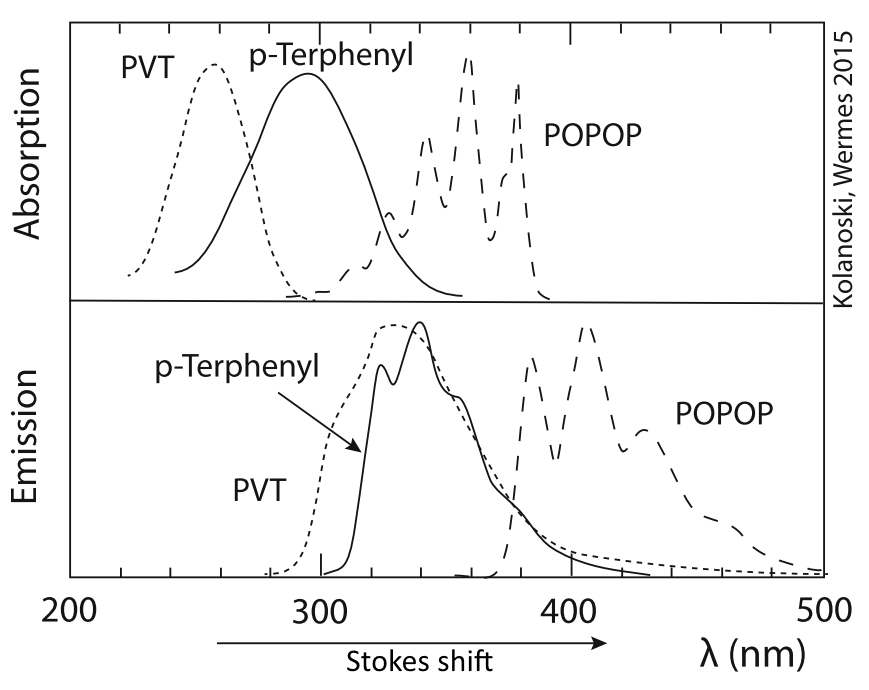
\includegraphics[width=0.5\textwidth]{./graphics/ch2/stokes2.png}}
\end{figure}
A quick coupling of three or more different components is necessary to provide sufficient speed. Between single molecules, this is done by the \tit{F\"orster resonance energy transfer} (FRET): the nonradiative excitation energy transfer by a long-range dipole dipole coupling mechanism \cite{FRET} ensures fast energy transfer from the basic material to the wavelength shifter. \par 
For minimal ionizing particles, the \tit{specific fluorescence} $\dv{S}{x}$, proportional to the light yield, can be estimated as the \tit{specific ionization} \cite{wermes}
\begin{align}
\dv{S}{r}=A\dv{E}{x}
\end{align}   
where $\dv{E}{x}$ is the specific energy loss \eqref{eq:bethe_bloch} with a proportionality factor A. For slower particles with higher energy loss, the production of quenching agents (damaged molecules) along the ionization trail of the particle has to be considered. A high ionization density deteriorates further excitation probability. The capture probability of a quenching agent relative to an undamaged molecule is given by $k_B$ (not to be confused with the Boltzmann factor). Considering this, an empirical formula, \tit{Birks law}, is given by \cite{birks}:
\begin{align}
\dv{S}{x}=\frac{A\cdot\dv{E}{x}}{1+k_B\dv{E}{X}}.
\end{align}     
For massive ionizing particles (high $\dv{E}{x}$), like fast $\alpha$-particles and heavier ions, the specific fluorescence can be described by $\dv{S}{x}=\frac{A}{k_B}$. 


\section{Inorganic scintillators}
The scintillation aspects of inorganic scintillators are given by the characteristics of the crystal lattice and electronic band structure.
\subsection{Electronic band structure} \label{ch:semiconducters} 
A \tit{crystal} is a material with a highly ordered microscopic structure, forming a lattice extending in all directions. The energy states of single atoms in the lattice are influenced by the periodic structure and form \tit{energy bands} which are separated by \tit{band gaps}. \par 
The electric conductivity is given by the two highest bands, the \tit{valence} and \tit{conduction band}. Metals in general have a good conductivity since the conduction and valence band overlap, valence electrons can directly change into the highest band and delocalize as \tit{electron gas}, providing good conductivity as free charge carriers. \tit{Semiconductors} have band gaps ranging from few hundredths of $\si{\eV}$ up to $\SI{9}{\eV}$ \cite{wermes}. \tit{Insulators} have band gaps with $>\SI{9}{\eV}$. A comparison is shown in figure \ref{fig:ch2:band_gaps}.    
\begin{figure}[b]
	\floatbox[{\capbeside\thisfloatsetup{capbesideposition={left,center},capbesidewidth=3.5cm}}]{figure}[\FBwidth]
	{\caption[Electronic band structure]{Electronic band structure for insulators (left), semiconductors (middle) and conductors (right). Amended from \cite{wermes}.}   
		\label{fig:ch2:band_gaps}}
	{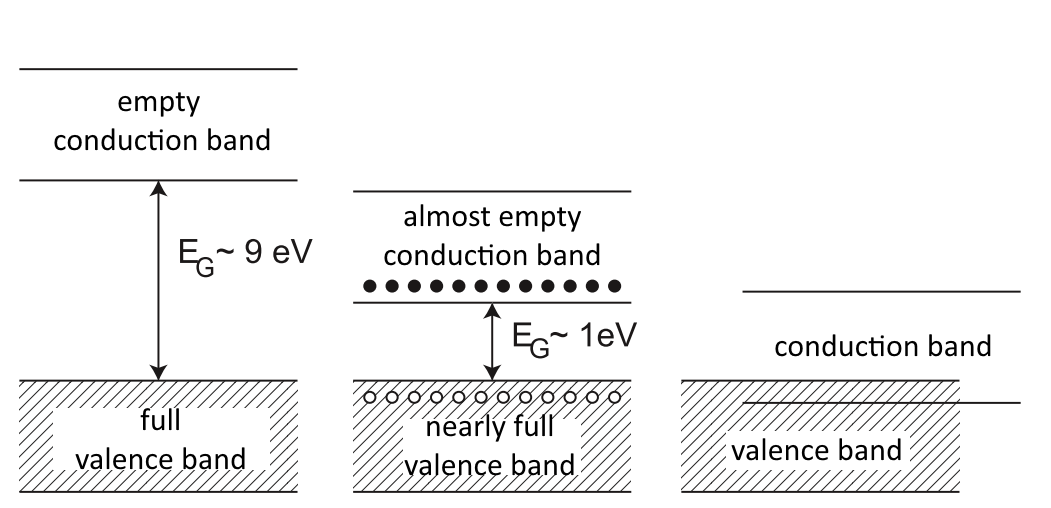
\includegraphics[width=0.75\textwidth]{./graphics/ch2/band_gaps.png}}
\end{figure}
The band gap of a scintillator lies roughly between $\SI{4}{\eV}$ and $\SI{12}{\eV}$. \par 
The creation of scintillation light is done by absorption of energy, exciting electrons from the valence band to the conduction band and relaxing back via photon emission. These processes are numerous and some will be discussed below.
\subsection{Creation of electron-hole pairs}
According to \cite{rodnyi}, the creation and annihilation of \tit{electron-hole pairs} can be separated into four stages. \par 
First, an incident particle creates and electron-hole pair by transferring energy to a bound electron, exciting it to the conduction band. The depth of the corresponding hole (usually in an inner shell) depends on the particles energy. \par 
The second stage describes the relaxation of both electrons and holes. Deep holes (in core shells) can relax by emitting radiation or nonradiative due to the \tit{Auger effect}, creating a new electron. The electron created in the first place loses energy because of inelastic electron-electron scattering. \par 
In the thermalization stage, the electrons and holes have not enough energy left for further ionization. Electrons move down to the edge of the conduction band, holes rise to the top of the valence band. \par 
The last stage describes the creation of scintillation light by excitation of \tit{luminescence centers}.
\subsection{Luminescence centers}
The energy states of the luminescence centers are smaller than the band gap of the scintillator. Hence, the optical emission spectrum is Stokes shifted to avoid reabsorption. \par 
\begin{figure}[t]
	\floatbox[{\capbeside\thisfloatsetup{capbesideposition={right,center},capbesidewidth=6.5cm}}]{figure}[\FBwidth]
	{\caption[Luminescence center]{Energy states of luminescence centers \cite{wermes}. The excitation (\ft{A}{C}) relaxes either due to thermal relaxation (\ft{C}{B}) or nonradiative transition ($F$). The luminescence transition is \ft{B}{D}. Since the energy for \ft{B}{D} is smaller than \ft{A}{C}, the emission spectrum is stokes shifted.}   
		\label{fig:ch2:luminescence}}
	{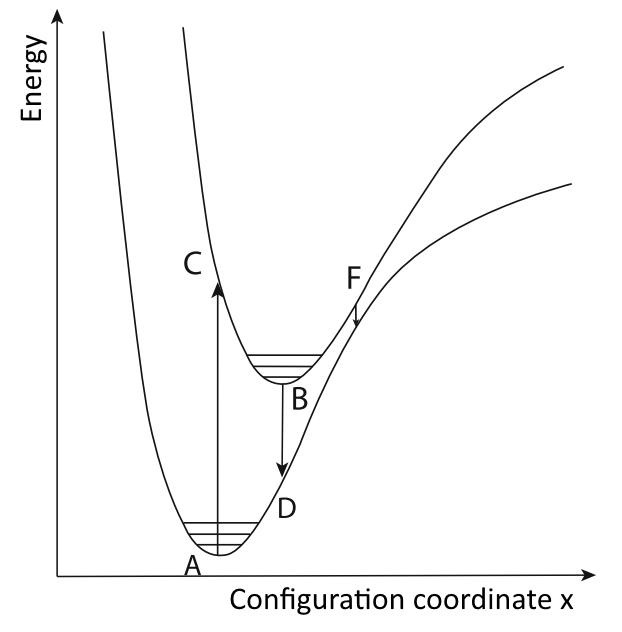
\includegraphics[width=0.5\textwidth]{./graphics/ch2/lum_center.png}}
\end{figure}
These centers can be intrinsic due to radiation damage or extrinsic by doping with activators to manipulate local electronic configurations. This improves the light yield.\par 
In figure \ref{fig:ch2:luminescence} the potential of a luminescence center is shown. Because of local polarization and thermal effects, the energy states are slightly shifted \cite{wermes}. The excitation of a center by \tit{excitons} (coupled electron-hole pairs) or absorption of electrons and holes follows the \tit{Franck-Condon principle}. It states, that transitions to corresponding vibrational states with minimal change in the nuclear number are favored \cite{franck}. This results in a higher excitation. After a thermal relaxation into the excited ground state, the center relaxes under emission of a photon. A nonradiative relaxation (quenching) is possible when the energy bands are close and thermal exchange through phonon coupling is likely. 
\subsection{Time scales}
The different time scales of the scintillation process of an intrinsic scintillator are illustrated in figure \ref{fig:ch2:time_scales} \cite{Lecoq}.
\begin{figure}[b!]
	\centering
	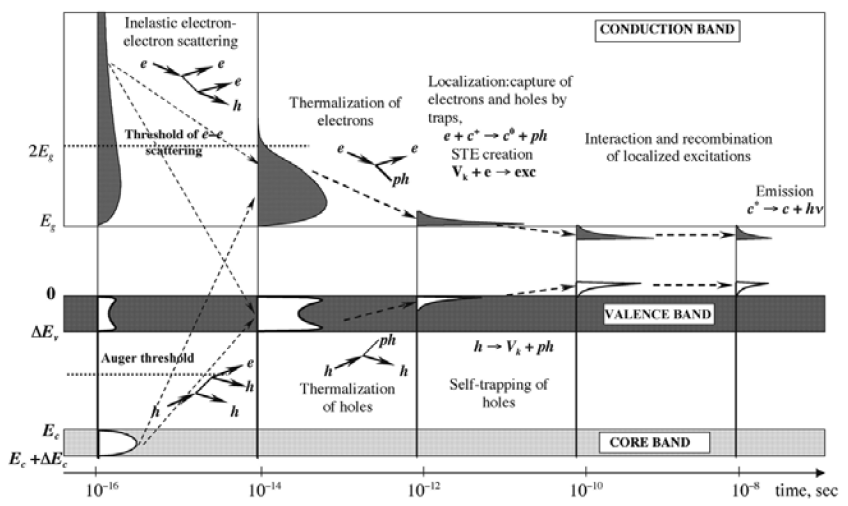
\includegraphics[width=0.85\textwidth]{./graphics/ch2/time_scales.png}
	\caption[Time scales of luminescence in inorganic scintillators]{Time scales of the scintillation process of an intrinsic organic crystal \cite{Lecoq}. Explanations can be found in the text.}   
	\label{fig:ch2:time_scales}
\end{figure}
After creating a deep core hole and exciting the corresponding electron, the energy is dissipated within $10^{-16}$ $\si{\second}$ to $10^{-14}$ $\si{\second}$ via electron-electron scattering, respectively Auger effect. Beneath a certain threshold, thermalization by phonon scattering dominates (up to $10^{-12}$ $\si{\second}$). On scales of $10^{-10}$ $\si{\second}$ to $10^{-8}$ $\si{\second}$, the charge carriers activate a luminescence center which subsequently emits scintillation light. \par     
Because of localization effects and impurities, \tit{trapping centers} can shortly trap a hole or an electron. Thermalization can release it after some hundreds of picoseconds. The thermalization of holes and excitons can be delayed by self-trapping which arises due to interaction with local phonons \cite{rodnyi}. \par
Another fast mechanism is the \tit{deep core luminescence}: if the absorption of energy creates a deep hole in the core band and the band gap between valence and conduction band is high ($>\SI{7}{\eV}$), then an ultra fast recombination (some hundred picoseconds) with a valence electron under emission of an optical photon is likely \cite{wermes}. Most of these crystals possess this fast and the conventional slow component, a prominent example being \baf.   
\section{Comparison and applications}
Since diverse applications require a variety of different properties, many scintillators have been developed. Some of the most important characteristics will be discussed. A short overview is given in table \ref{ch2:tab:characteristics}. \par 
As stated before, scintillators are produced in many different geometries. The organic plastics, above all, can be cast in various shapes. The inorganic crystals are limited in size and geometry by the growing method. Crystals are mostly produced as bars or cylinders. \par  
The speed of the scintillation process depends on the particular mechanism. Generally, plastics are faster than crystals, whereas some exceptions exist (\baf). Due to material, production process and size, the costs vary strongly. \par 
The radiation length and density are key factors for some applications. For timing purposes the particles should not be influenced, hence less dense materials, i.e. plastics, are valid. Energy measurements require a dense material able to stop particles within a small area, therefore crystals are used. \par 
The peak emission wavelength $\lambda_{em}$ and light yield are key factors for choosing an adequate photodetector. They play a crucial role in application: for timing, one needs only few photons whereby energy measurements need a great number of photons for sufficient precision. \par 
In medical applications (PET, CT), $\gamma$-spectroscopy, energy measurements in high energy physics and radiation monitoring, crystals are state-of-the-art. Plastics are often used for timing, time-of-flight measurements and detection of charged particles, e.g. cosmic rays.

\begin{table}[b]
	\centering
	\begin{tabular}{ cccccccc } \toprule[2pt]
		Material & $\rho$ [$\si{\gram}/\si{\cubic\centi\meter}$] & $\lambda_{em}$ [$\si{\nano\meter}$] & L$_{S}$ & $\tau_{decay}$ [$\si{\nano\second}$] & $\mu$ [$\si{\centi\meter}$] & $X_0$ [$\si{\centi\meter}$] & Src \\ \midrule
		EJ-248M & 1.023 & 425 & 9200 & 2.1 & 250 & $-$ &  \cite{eljen}\\
		EJ-204  & 1.023 & 408 & 10400 & 1.8 & 160 & $-$ & \cite{eljen}\\
		EJ-301  & 0.874 & 425 & 12000 & 3.2 & 3000 & $-$ & \cite{eljen} \\ 
		NaI(Tl) & 3.670 & 415 & 38000 & 250 & $-$ & 2.59 & \cite{saint-gobain} \\
		BGO & 7.130 & 480 & 10000 & 300 & $-$ & 1.14 & \cite{saint-gobain} \\
		\baf & 4.880 & 195/310 & 1800/10000 & 0.8/630 & $-$ & 2.03 & \cite{saint-gobain} \\
		LYSO & 7.100 & 420 & 30000 & 45 & $-$ & 1.20 & \cite{saint-gobain} \\
		\pwo & 8.280 & 425 & 130 & 30 & $-$ & 0.89 & \cite{wermes} \\ \bottomrule[2pt]
	\end{tabular}
	\caption[Comparison of different scintillators]{Comparison of different scintillators. The first two are plastics, the third one is liquid, the last four are solid crystals. Note that BaF$_2$ has two scintillation components. $\mu$ is the light attenuation coefficient (see \eqref{eq:beer_lambert}).}
	\label{ch2:tab:characteristics}
\end{table}































\chapter{Photodetectors} \label{ch:photo_detectors}
As depicted in chapter \ref{ch:scintillators}, the detection of scintillation light is a crucial task when it comes to building detectors. Before semiconductor detectors like the \tit{photodiode} were invented, the \tit{photomultiplier tube} (PMT) was state-of-the-art for measuring up to single photons with low noise and high gain. Although PMTs are widely used, photodiodes provide attractive advantages in some cases. A short overview and comparison is given in this chapter. 
\section{Photomultiplier tube}
The photomultiplier tube is an evacuated glass tube with internal electronic structures. At the front, a photo cathode converts an incident photon from the light input window via the photoelectric effect into a photoelectron.  
\begin{figure}[b]
	\floatbox[{\capbeside\thisfloatsetup{capbesideposition={right,center},capbesidewidth=6.5cm}}]{figure}[\FBwidth]
	{\caption[Photomultiplier tube]{Cross section of a photomultiplier tube. The base for the PMT is mounted onto the pins on the bottom of the glass tube. Amended from \cite{wermes}.}   
	\label{fig:ch3:pmts}}
	{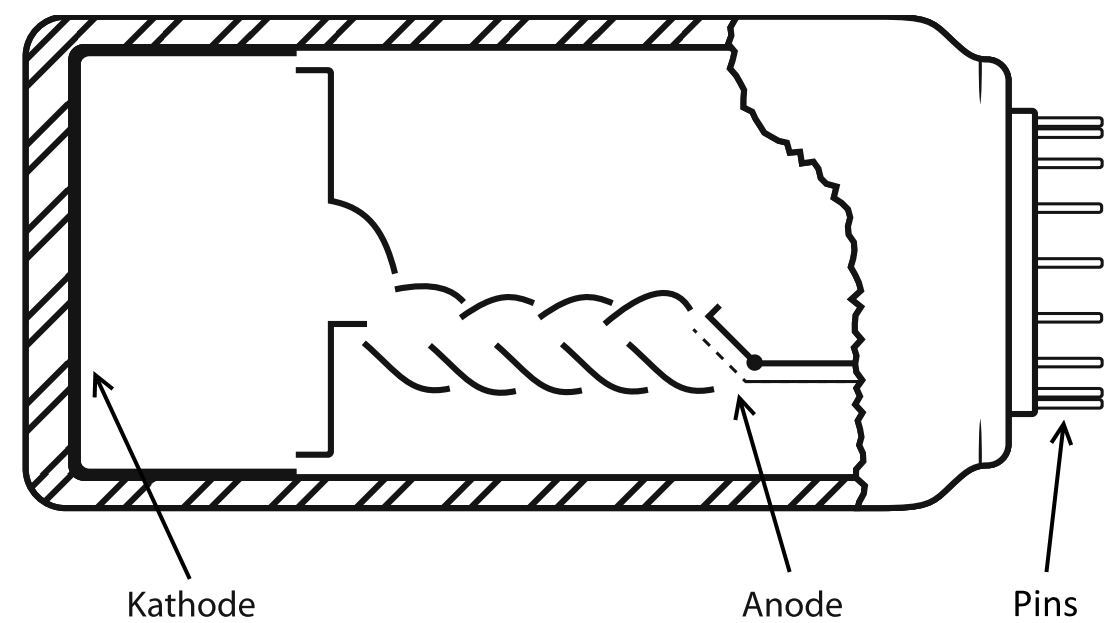
\includegraphics[width=0.5\textwidth]{./graphics/ch3/pmt1.png}}
\end{figure}
A strong electric field accelerates this electron, focused by a focusing element, towards a first electron multiplier (\tit{dynode}). The impact creates a cascade of secondary electrons which are then accelerated towards a sequence of dynodes. These structures can bee seen in figure \ref{fig:ch3:pmts}. After a \tit{transit time} of few tens of nanoseconds \cite{moore} the shower of electrons, now amplified by a factor of $10^{5}$ to $10^{9}$, reaches the anode where a measurable electric pulse is generated. \par 
A resistive voltage divider (\tit{dynode-chain} or simply \tit{base}) supplies the accelerating voltages for the dynodes and is attached to the pins on the bottom of the glass tube. In order to create sufficient acceleration, high-voltage (500$\si{\volt}$-2500$\si{\volt}$) is used. \par 
The \tit{quantum efficiency} (QE) describes the probability whether an incident photon is converted into a photoelectron or not. This ratio depends on the \tit{photocathode radiant sensitivity} (QS) which is defined as the quotient of incoming energy $N_{ph}\cdot h\nu$ and converted energy $N_{pe}\cdot e$:
\begin{align}
QS=\frac{N_{pe}\cdot e}{N_{ph}\cdot h\nu} \left[\si{\ampere\second\over\watt\second}\right].
\label{eq:quantum_efficieny_pmt}
\end{align} 
Typical quantum efficiency values vary between 25\% and 40\%. These values highly depend on the material used for the entrance window and the photocathode. Figure \ref{fig:ch3:pmt_sensitivity} illustrates the quantum efficiency for different wavelengths. For instance, measuring the fast scintillating component of BaF$_2$ necessitates the usage of a fused silica light input window with a bialkali photocathode. \par 
Albeit PMTs have a high gain, fast amplification, low noise and single photon sensitivity, they cannot be used in strong magnetic fields. Yet they can be operated in low fields by shielding with $\mu$-metal. In addition, PMTs rely on high operating voltages and are bulky to mount on scintillators. \par 
Considering these downsides, one has to use other photodetectors when it comes to strong magnetic fields, space constraints and low costs. These prerequisites can be found in medical applications (MRT) and high energy physics (large-scale detectors).
\begin{figure}[h!]
	\subfloat[Photocathode radiant sensitivity] {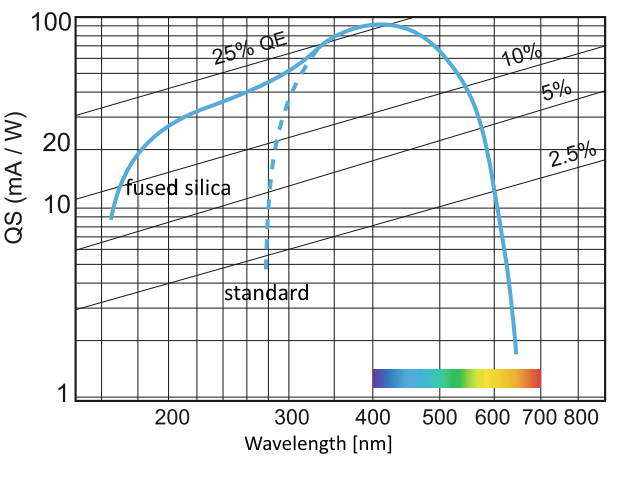
\includegraphics[width=0.49\textwidth]{./graphics/ch3/pmt_glass.png}}
	\hfill
	\subfloat[Photon emission spectra ] {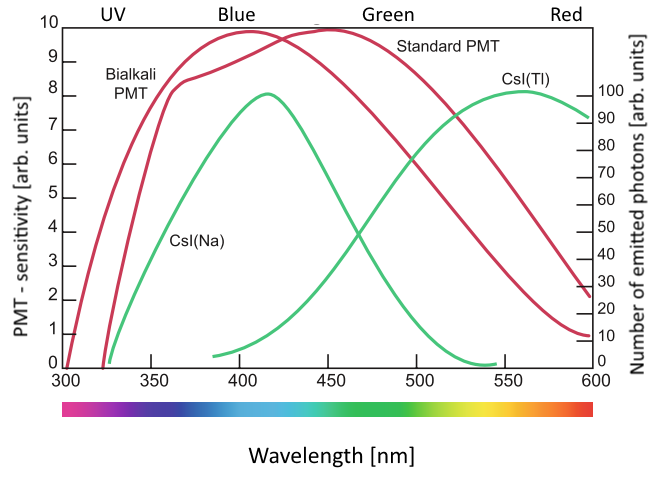
\includegraphics[width=0.49\textwidth]{./graphics/ch3/pmt_sensitivity.png}}
	\hfill
	\caption[Photon sensitivity of PMTs]{PMT wavelength dependency of photon sensitivity \cite{wermes}. The sensitivity for UV photons can be extended by using fused silica light input windows (a). To get the highest efficiency, the photocathode material has to be adapted for the emission spectrum of the scintillator (b).}
	\label{fig:ch3:pmt_sensitivity}
\end{figure} 
\section{Semiconductor detectors}
To solve some of the shortcomings of PMTs, solid state physics contributes a comprehensive class of materials, the semiconductors, which already have been introduced in chapter \ref{ch:semiconducters}. In the following, some applications will be presented.
\subsection{p-n junction}
The junction between a positive (p-) and negative (n-) doped semiconductor is called \tit{p-n junction}. In contact, free charge carriers (holes $h$ and electrons $e$) diffuse into the opposed region, leaving negative, respectively positive charged ions behind. Due to recombination, a \tit{depletion layer} between the p- and n-doped material is produced, which lacks free charge carriers. Since there are charged ions left, a \tit{built-in potential} forms and an electric field is generated (see figure \ref{fig:ch3:pn}). A stable condition attunes when the recombination stops and the drift and diffusion of holes and electrons compensate.   \par 
With \tit{reversed bias} (positive terminal attached to the cathode), the depletion layer broadens and the built-in potential intensifies. At a certain level of voltage $U_{BD}$, an avalanche occurs where electrons gain sufficient energy to create more charge carriers (\tit{breakdown}).  \tit{Forward biasing} (positive terminal attached to the anode) will shrink the layer and therefore lower the electrical resistance.   \par 
The p-n junction, as part of a circuit, is called \tit{diode}. 
\begin{figure}[h!]
	\floatbox[{\capbeside\thisfloatsetup{capbesideposition={right,center},capbesidewidth=6.75cm}}]{figure}[\FBwidth]
	{\caption[p-n junction]{Schematics of a p-n junction. It can be seen that the energy levels in the contact region are curved due to the different doping. The Fermi level adjusts to stay constant. The depletion layer inhibits positive and negative ions which produce an electric field. It is oriented from the n- to the p-junction. In equilibrium, the net currents of drifting and diffusing are equal.  Graphic amended from \cite{wermes}.}   
		\label{fig:ch3:pn}}
	{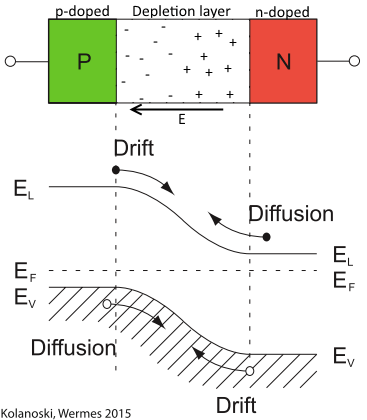
\includegraphics[width=0.5\textwidth]{./graphics/ch3/pn.png}}
\end{figure}

\subsection{Photodiode}

The design of a photodiode is based on the p-n junction structure with reverse biasing. Incident photons with sufficient energy excite an electron-hole pair in the depletion region, which is then separated due to the electrical field. Both charge carriers get accelerated towards their respective electrode and an electric pulse can be measured because of induction. \par 
A so called \tit{p-i-n} diode is shown in figure \ref{fig:ch3:diode}. An intrinsic sheet is placed between p- and n-doped layers. By applying reverse bias, a depletion region forms across the whole intrinsic sheet which then provides electron-hole pairs by photoexcitation. \par 
Made of silicon, a photodiode has a higher quantum efficiency and sensitivity on a wider wavelength spectrum compared to PMTs, although they have no intrinsic amplification, a smaller sensitive surface and rely on preamplifiers. To overcome some of these downsides, the \tit{Avalanche Photo Diode} (APD) was developed. \par
\begin{figure}[b]
	\floatbox[{\capbeside\thisfloatsetup{capbesideposition={left,center},capbesidewidth=0.35\linewidth}}]{figure}[\FBwidth]
	{\caption[Photodiode]{Cross section of a photo diode. For reverse biasing, the cathode is connected to the positive terminal. Amended from \cite{wermes}.}   
		\label{fig:ch3:diode}}
	{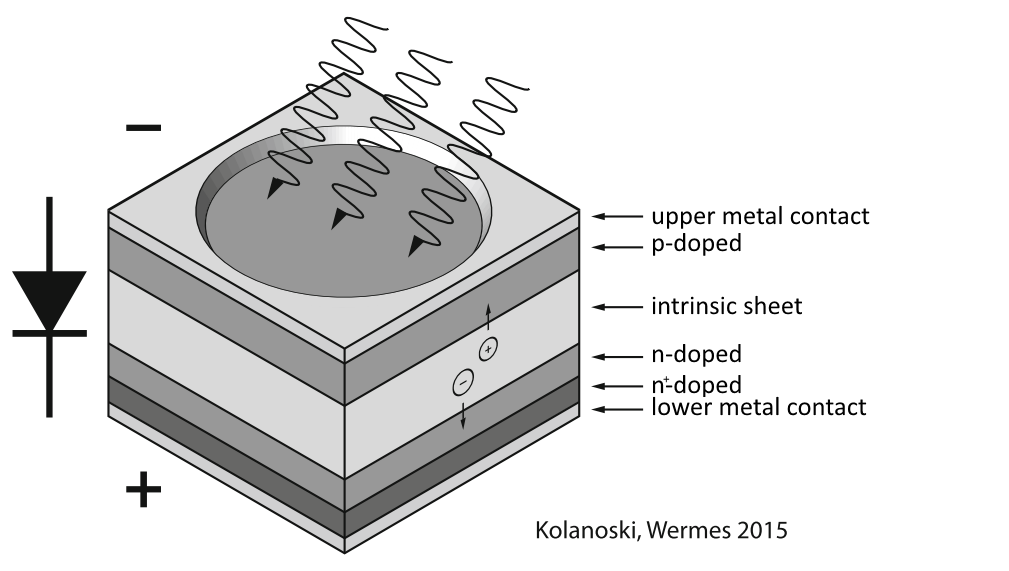
\includegraphics[width=0.65\textwidth]{./graphics/ch3/diode.png}}
\end{figure}
In addition to a single p-n junction, the APD integrates a second \tit{metallurgical junction} (highly doped p-n barrier junction) within the metal contacts. Incident photons excite h-e pairs in a thick, less-doped depletion region. The produced electrons drift through the depletion layer towards the readout electrode and pass the metallurgical junction. Since this barrier has a high electric field (up to $\SI{1}{\keV/\milli\meter}$ \cite{wermes}), the passing electrons gain energy and create secondary charge carriers through impact ionization processes. This avalanche continues and amplifies the signal up to a factor of \ten{2} to \ten{3}. \par 
To gain even higher amplification (up to \ten{5}), \tit{single photon APDs} (SPADs) can be operated in \tit{Geiger-Mode} where the supplied voltage $U_{OP}$ is set to 10\%-20\% beyond breakdown voltage $U_{BD}$. A single photon can trigger a self-perpetuating ionization cascade, the \tit{Geiger discharge}. To avoid any damage and to reset the APD, a series \tit{quenching resistor} $R_Q$ is used.  

\subsection{Silicon photomultiplier}

The \tit{Silicon Photomultiplier} (SiPM) integrates a large number of microcells ($\text{SPAD}+R_Q$) as an array in a dense area on a silicon substrate \cite{sensL}. The SPAD pixel size ranges from $\SI{15}{\micro\meter}$ to $\SI{70}{\micro\meter}$ \cite{buzhan}. Each pixel works binary, therefore the number of incident photons can be estimated by the number of pixels hit. The probability of multiple hits of a single cell is low since the packing density is high and the dead time is small ($<\SI{100}{\nano\second}$ \cite{wermes}). \par 
\begin{figure}[b!]
	\subfloat[N-on-P structure.] {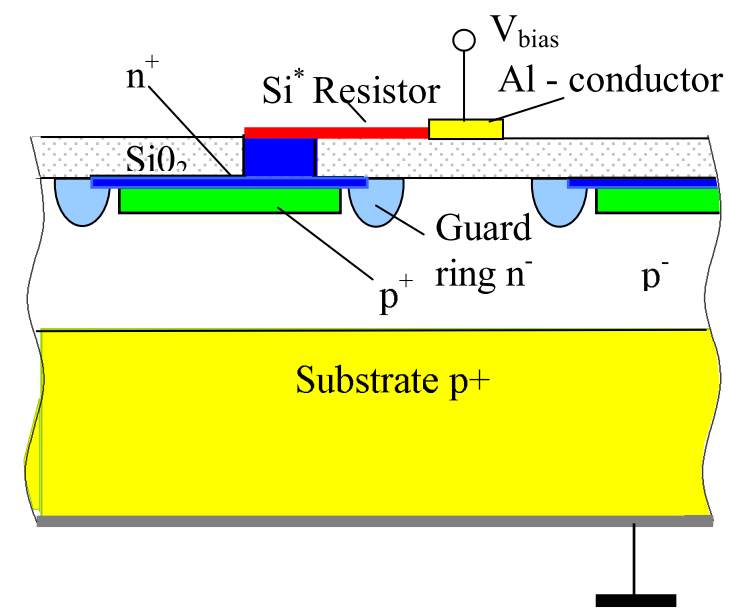
\includegraphics[width=0.45\textwidth]{./graphics/ch3/sipm_scheme.png}}
	\hfill
	\subfloat[\tit{KETEK} \tit{P-on-N} structure] {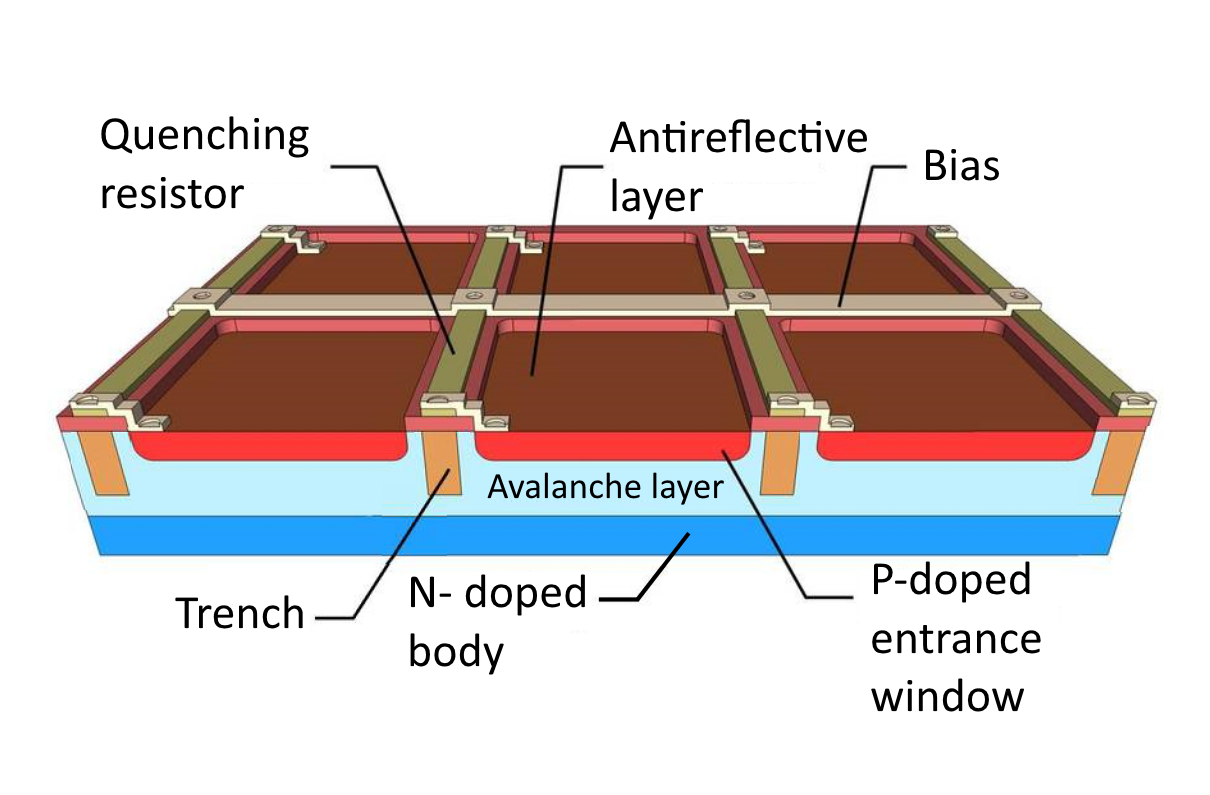
\includegraphics[width=0.54\textwidth]{./graphics/ch3/ketek_sipm_scheme.png}}
	\hfill
	\caption[SiPM schematics]{Different schematics of SiPM designs. N-on-P technology with guard-rings (a). P-on-N technology with trenches to avoid cross-talk by \tit{KETEK} (b). Amended from \cite{buzhan} and \cite{ketek}. }
	\label{fig:ch3:sipm_scheme}
\end{figure}
In figure \ref{fig:ch3:sipm_scheme} some SiPM schematics are shown. Incident photons are absorbed in the depletion layer (blue photons within $\SI{0.6}{\micro\meter}$, red photons within $\SI{2.9}{\micro\meter}$ \cite{wermes}) and the excited electrons drift towards the avalanche layer, where the amplification with a factor of up to \ten{6} happens and a signal is induced. The use of \tit{guard rings} avoids occurrence of surface currents and trenches avert, in combination with anitreflective layers, \tit{optical cross-talk} (photons emitted by avalanches escaping into an adjacent cell) to reduce noise. \par 
Since SiPMs work with low voltage ($<\SI{80}{\volt}$) and 10\%-20\% over-voltage, an avalanche has to be quenched with a resistor. When current is drawn by this resistor, the voltage drops below the breakdown voltage, the avalanche stops and the cell recharges. This generates a pulse with a short rise time of $\approx\SI{0.5}{\nano\second}$ and a tail with few hundreds of nanoseconds. \par 
Some further characteristics are the \tit{fill factor} (percentage of surface sensitive to light), the \tit{photon detection efficiency} (PDE, sensitivity as function of wavelength), the \tit{dark count rate} (count rate without exposure to light), \tit{afterpulsing} (delayed release of trapped carriers after primary breakdown) and temperature dependencies.






\chapter{Silicon Photomultiplier characterization studies}
One major focus of this thesis is the characterization of SiPMs in terms of measuring IV-curves, determining the breakdown voltage and optimal working voltage, pulse shaping and comparing responses of different array setups.
\section{Development of a SiPM-board}
\begin{figure}[b!]
	\subfloat[SiPM Printed Circuit Board (PCB)] {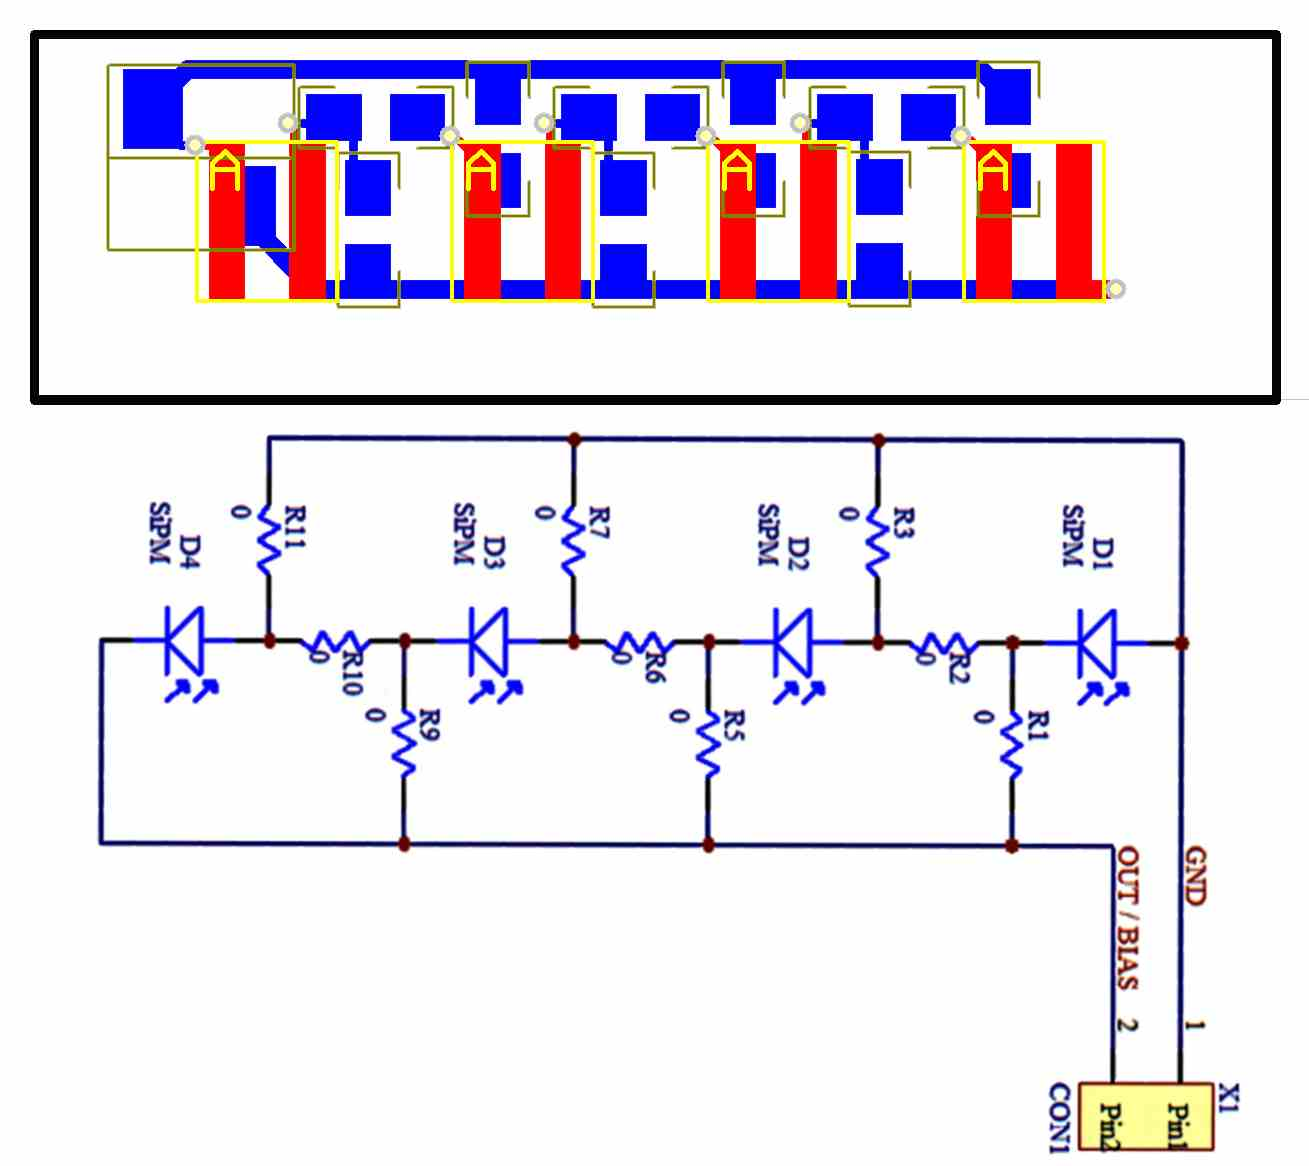
\includegraphics[width=0.49\textwidth]{./graphics/ch4/PCB.jpg}}
	\hfill
	\subfloat[SiPM circuit configurations \cite{sebastian}] {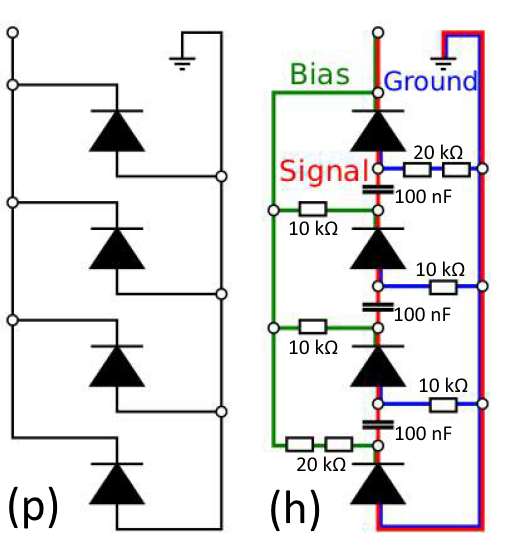
\includegraphics[width=0.4\textwidth]{./graphics/ch4/circuits.png}}
	\hfill
	\caption[SiPM circuit configurations]{SiPM board development.  }
	\label{fig:ch4:PCB}
\end{figure}
As a first approach, an electronic board for mounting different configurations of SiPMs has been developed. The PCB is shown in figure \ref{fig:ch4:PCB}. Note that this board allows different SiPM-configurations like single (s), parallel (p) and hybrid (h), the pros and cons of each will be discussed later. The design is inspired by the readout module for the scintillator tiles of the PANDA Barrel-TOF detector \cite{SciTil}. Figure \ref{fig:ch4:PCB} shows the PCB design and the circuit. A single SiPM is directly connected to the bias and ground without any passive parts. The parallel board integrates two till four SiPMs, each of them connected to the bias and ground in parallel. A fast, shaped signal is received when capacitors connect anode and cathode of adjacent SiPMs (hybrid) and resistors are used for connecting the SiPMs with bias and ground. The signal is coupled onto the DC bias voltage and can be separated via a capacitor.  \par 
For this thesis, \tit{KETEK} PM3350-EB were used. With an active area of $\SI{3}{\milli\meter}\times\SI{3}{\milli\meter}$ and a pixel size of $\SI{50}{\micro\meter}\times\SI{50}{\micro\meter}$ and 3472 pixels overall, the SiPM trades off a high photo detection efficiency and a good micro cell density. For further parameters, see \cite{SiPM_Manual}. \par
With a breakdown voltage of $U_{BD}=\SI{25}{\volt}$ and an operation voltage of $U_{OP}=U_{BD}+(2-7)\si{\volt}$, the (s)-configuration can be chosen for low cost and a fair light exposure, i.e. a plastic scintillator for measuring cosmic muons. The (h)-configuration promises good timing with a fast rising edge. It is meant for precise timing purposes, like time of flight measurements. An energy measurement can be done with the (p)-configuration, where the effective light-sensitive area is directly given by the sum of the SiPM surfaces. For some experiments, preamplifiers by \tit{Photonique} have been used \cite{photonique}.\par 

\section{Current$-$voltage characteristic}
\begin{figure}[b]
	\centering
	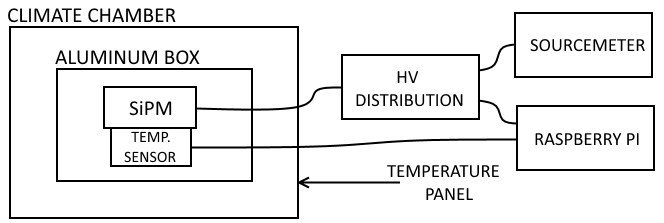
\includegraphics[width=0.85\linewidth]{./graphics/ch4/scheme_iv_curves.png}
	\caption{Schematic of the IV-characterization measurement setup.}
	\label{fig:ch4:iv_scheme}
\end{figure}
To determine the temperature dependence of the breakdown and optimal operation voltage, some IV-curve of arbitrarily chosen SiPMs in different configurations have been measured.  \par 
This setup is shown in figure \ref{fig:ch4:iv_scheme}: The climate chamber contains an aluminum box with the SiPM. The HV board \cite{chris}, which is currently under development for the EMC barrel of the PANDA experiment at FAIR (GSI) \cite{panda_emctdr}, has been chosen to perform the IV-scanning because of availability and easy programmability. The board is controlled by a Raspberry Pi 2 micro-computer which also reads out a temperature sensor  directly attached to the SiPM. To avoid parasitic light and surface leakage, the SiPM is cleaned with ethanol and is wrapped in black tape. A Keithley sourcemeter powers the HV board, a PC controls the Raspberry via Ethernet. The temperature settings can be set by a terminal. 
\begin{figure}[h!]
	\subfloat[(s)-configuration] {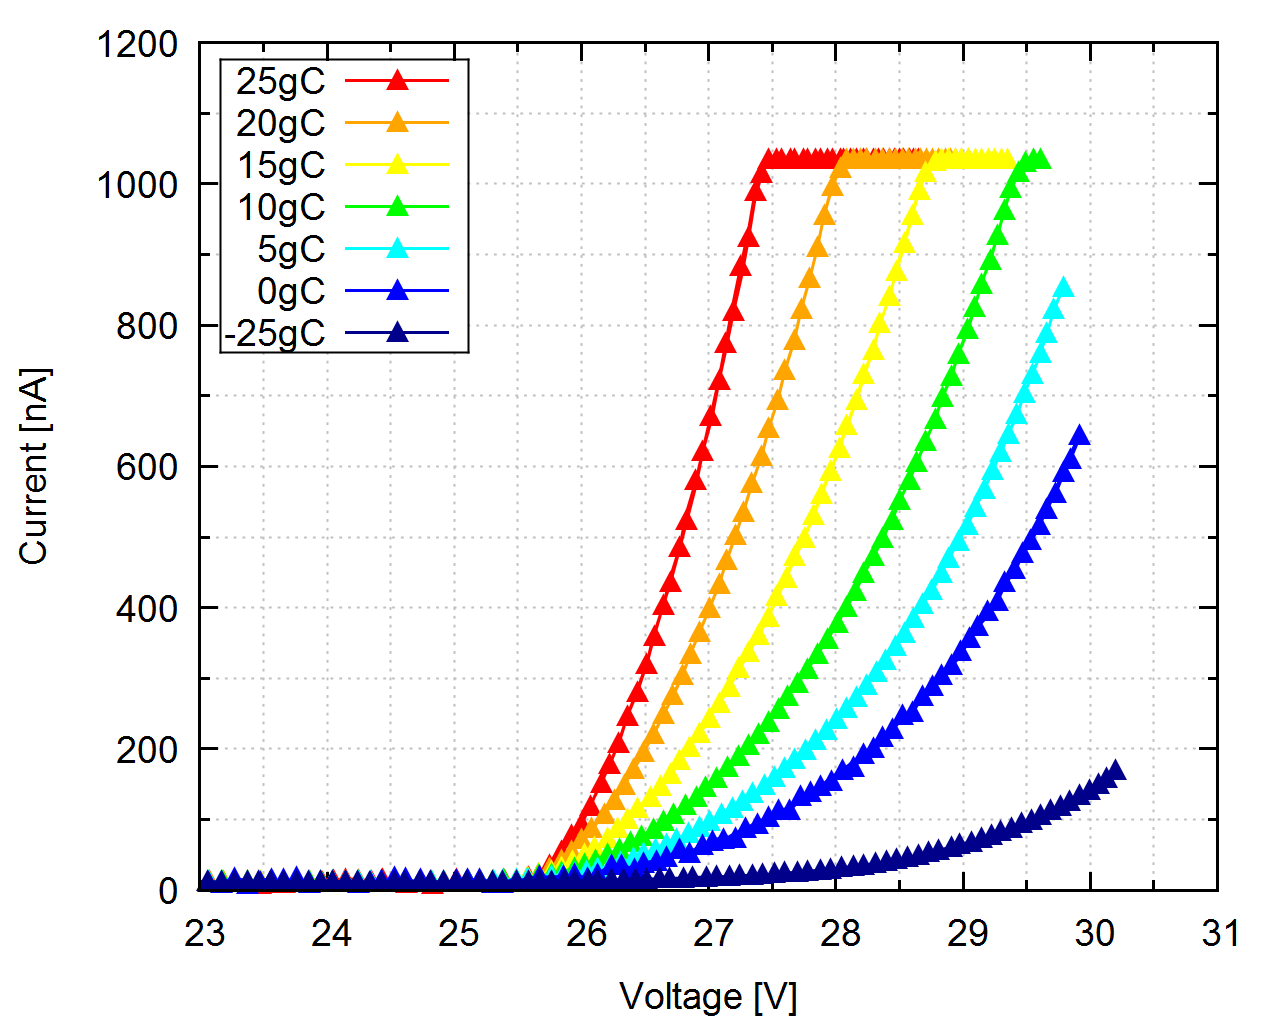
\includegraphics[width=0.49\textwidth]{./plots/iu_curve/1x1n2.png}}
	\hfill
	\subfloat[(s)-configuration logscale] {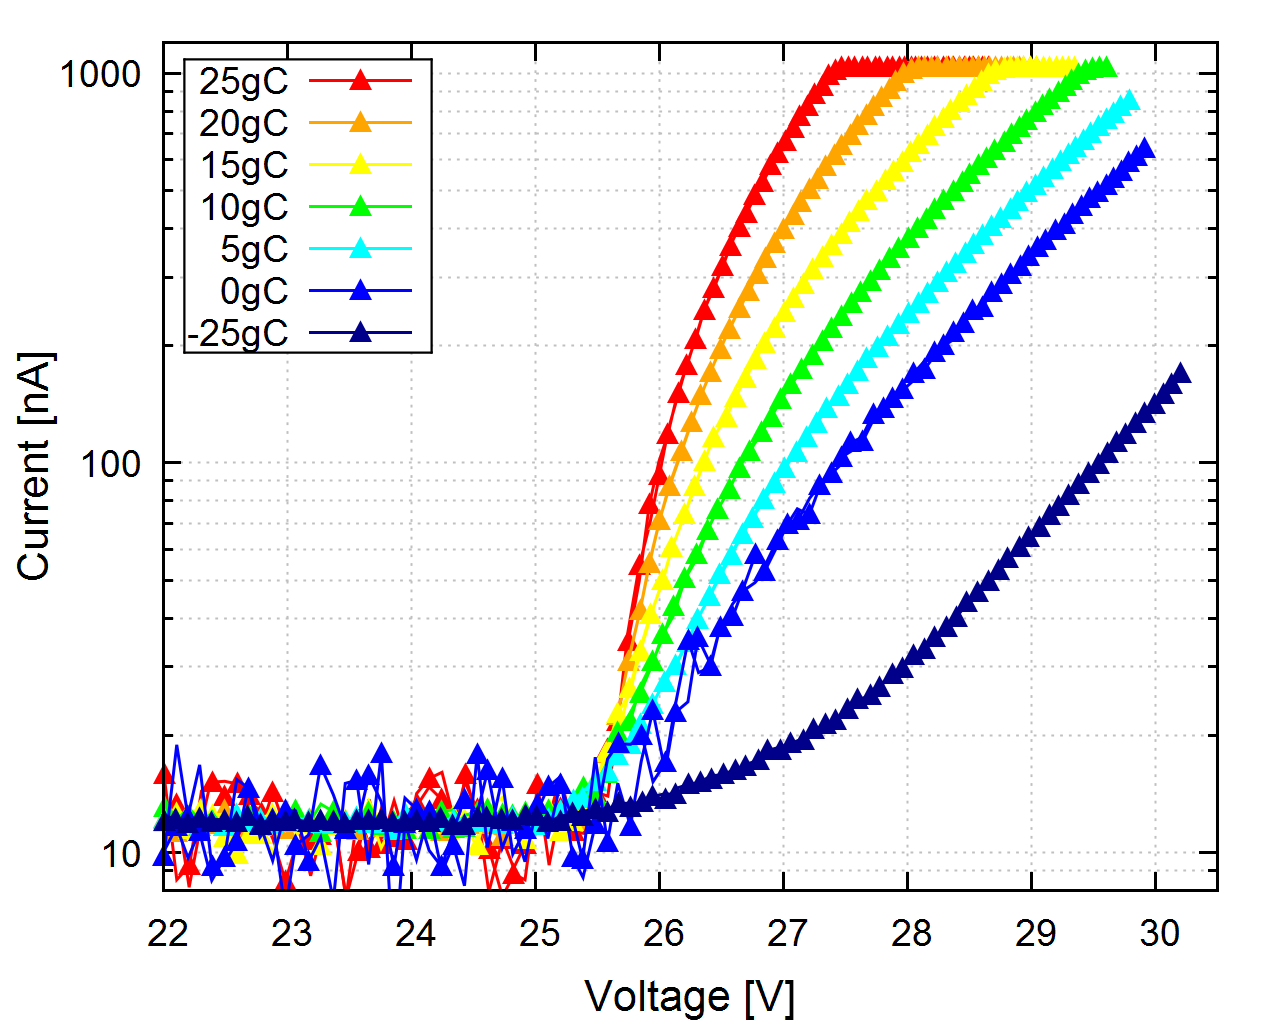
\includegraphics[width=0.49\textwidth]{./plots/iu_curve/1x1n2_log.png}}
	\hfill
	\subfloat[(h)-configuration] {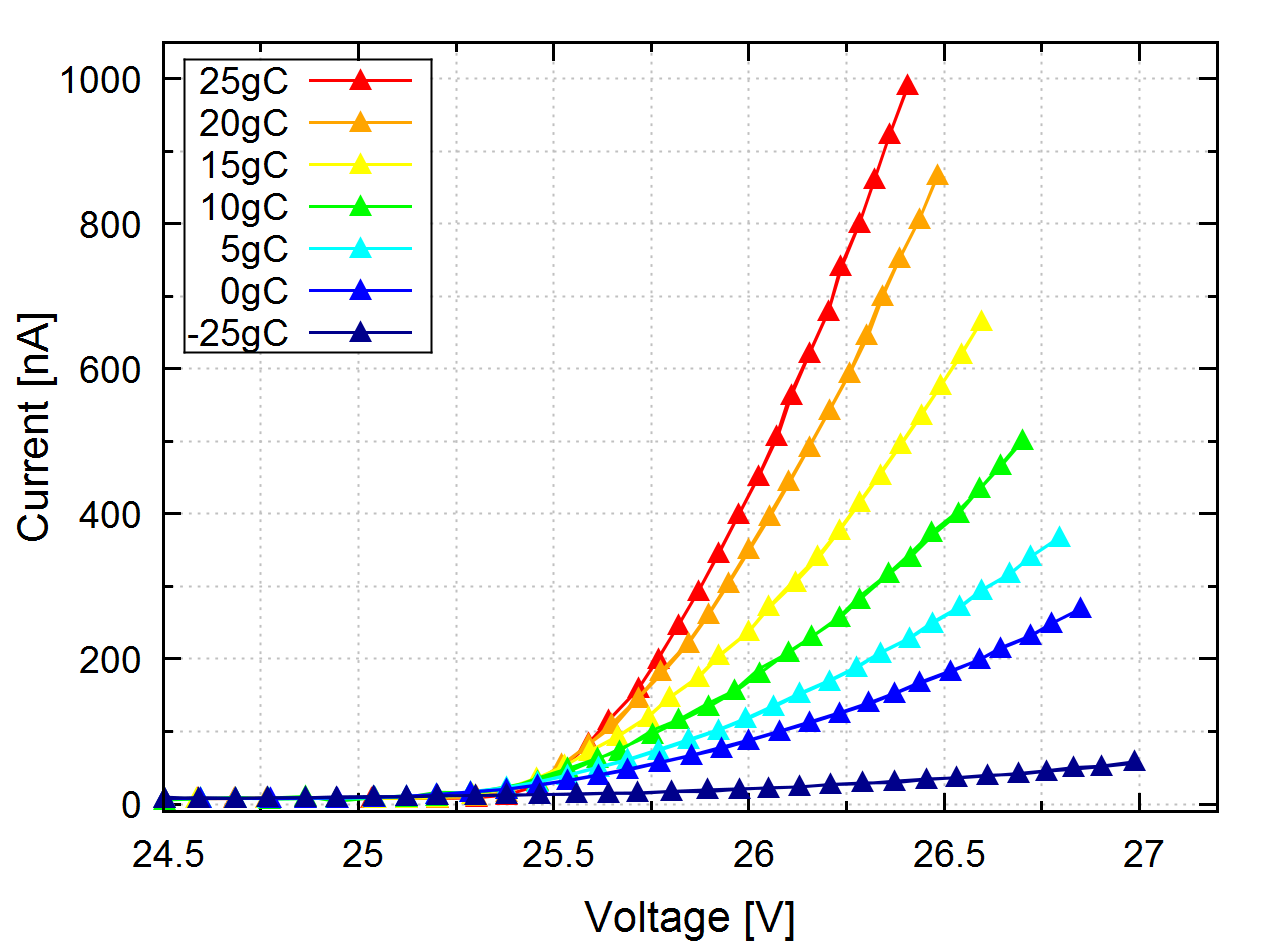
\includegraphics[width=0.49\textwidth]{./plots/iu_curve/4x1n6.png}}
	\hfill
	\subfloat[(h)-configuration logscale] {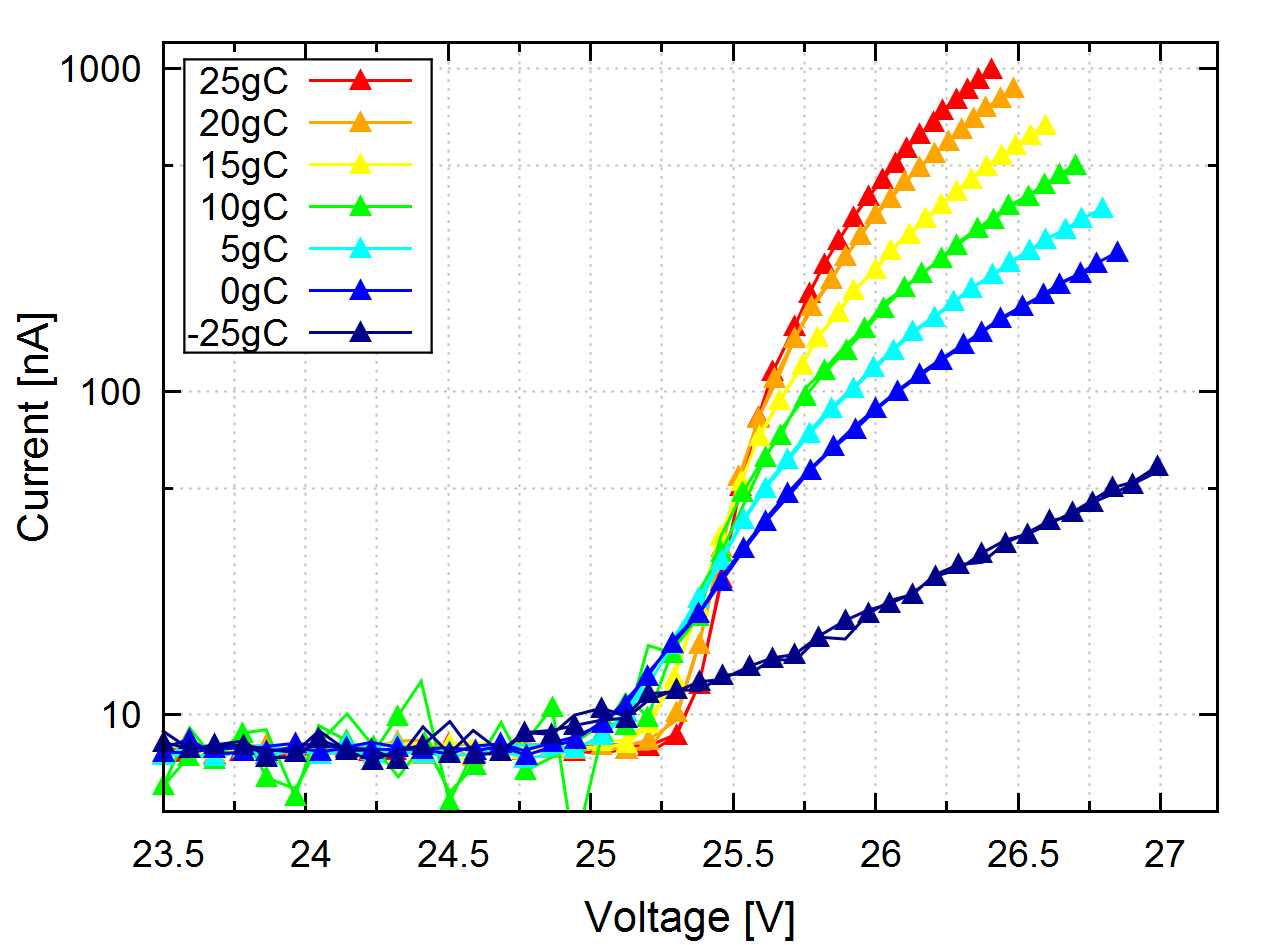
\includegraphics[width=0.49\textwidth]{./plots/iu_curve/4x1n6_log.png}}
	\hfill
	\subfloat[(p)-configuration] {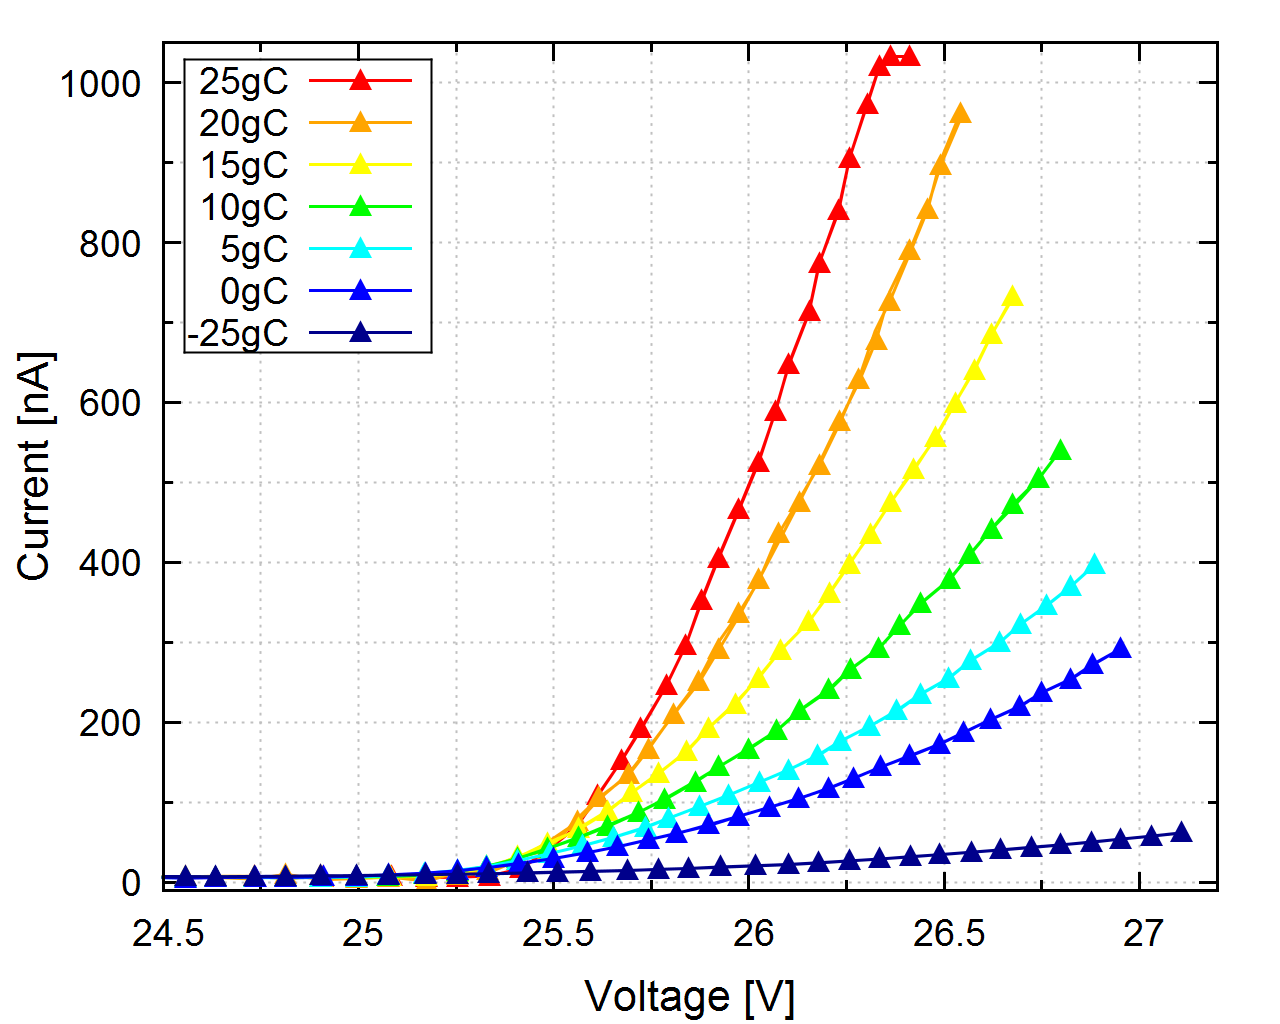
\includegraphics[width=0.49\textwidth]{./plots/iu_curve/4x1n6p.png}}
	\hfill
	\subfloat[(p)-configuration logscale] {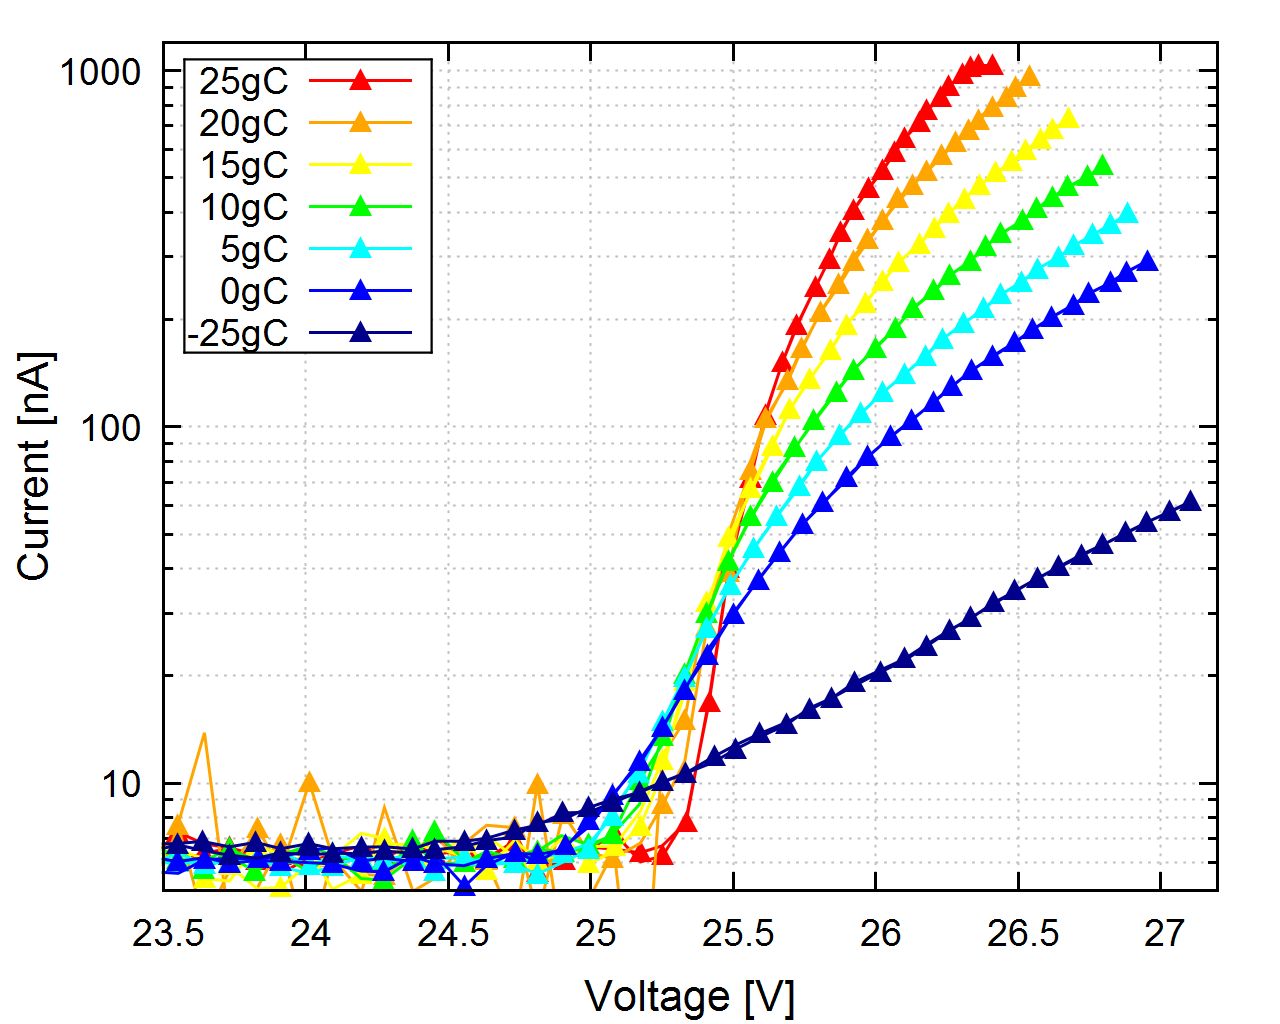
\includegraphics[width=0.49\textwidth]{./plots/iu_curve/4x1n6p_log.png}}
	\hfill
	\caption[IV-curve of different board configurations]{Comparison of different board configurations. For (h)- and (p)-configuration the same SiPMs were used. }
	\label{fig:ch4:IV_comparison}
\end{figure}
The IV-curves were scanned from $I=\SI{0}{\nano\ampere}$ to $I\approx\SI{1000}{\nano\ampere}$ and back to $I=\SI{0}{\nano\ampere}$. The step range is given by the digital potentiometer (10bit) on the HV board, a small hysteresis for the current is known (see \cite{chris}). For each potentiometer position (voltage), the current is measured 100 times and is then averaged. This results in two IV-curves per SiPM which should improve precision. It has to be mentioned that the voltage and current measurements are not fully calibrated yet, so a small offset might occur. This is not considered in this thesis, since qualitative comparison between the boards is sufficient.  \par 
The IV-curves for the different configurations are shown in figure \ref{fig:ch4:IV_comparison}. Plot (a) and (b) show the curves of a single SiPM. The temperature is color coded from warm (red) to cold (dark blue). It can be seen that the current rises exponentially when the breakdown voltage is exceeded. At this point, the local field strength is high enough to create avalanches. This process is temperature dependent: for lower temperatures, the generation of thermal electrons as free charge carriers able to start an avalanche is suppressed. \par 
The temperature also affects the breakdown voltage. A negative breakdown coefficient $k$ (in [$\si{\milli\volt\per\kelvin}$]) occurs in \tit{Zener diodes}: due to high doping, the band structures are heavily curved and show a steep slope. For higher temperatures, an electron can tunnel from the valence to the conduction band more easily. For avalanche diodes a positive $k$ is observed. Lower temperature suppresses electron-phonon scattering which increases the \tit{mean free path} (average distance between collisions) of electrons. This facilitates the development of avalanches and leads to a reduced breakdown voltage.\par 
Compared to a single SiPM, the parallel and hybrid configurations show higher currents. Each SiPM in the array is driven with the same voltage and contributes a net current to the overall current. Hence, the current should be the sum of the net currents. Therefore, breakdown and operation voltage can not be adjusted for each SiPM in an array but has to be treated altogether. This will be discussed later.

\section{Breakdown and operation voltage}


\begin{figure}[t]
	\subfloat[(s)-configuration] {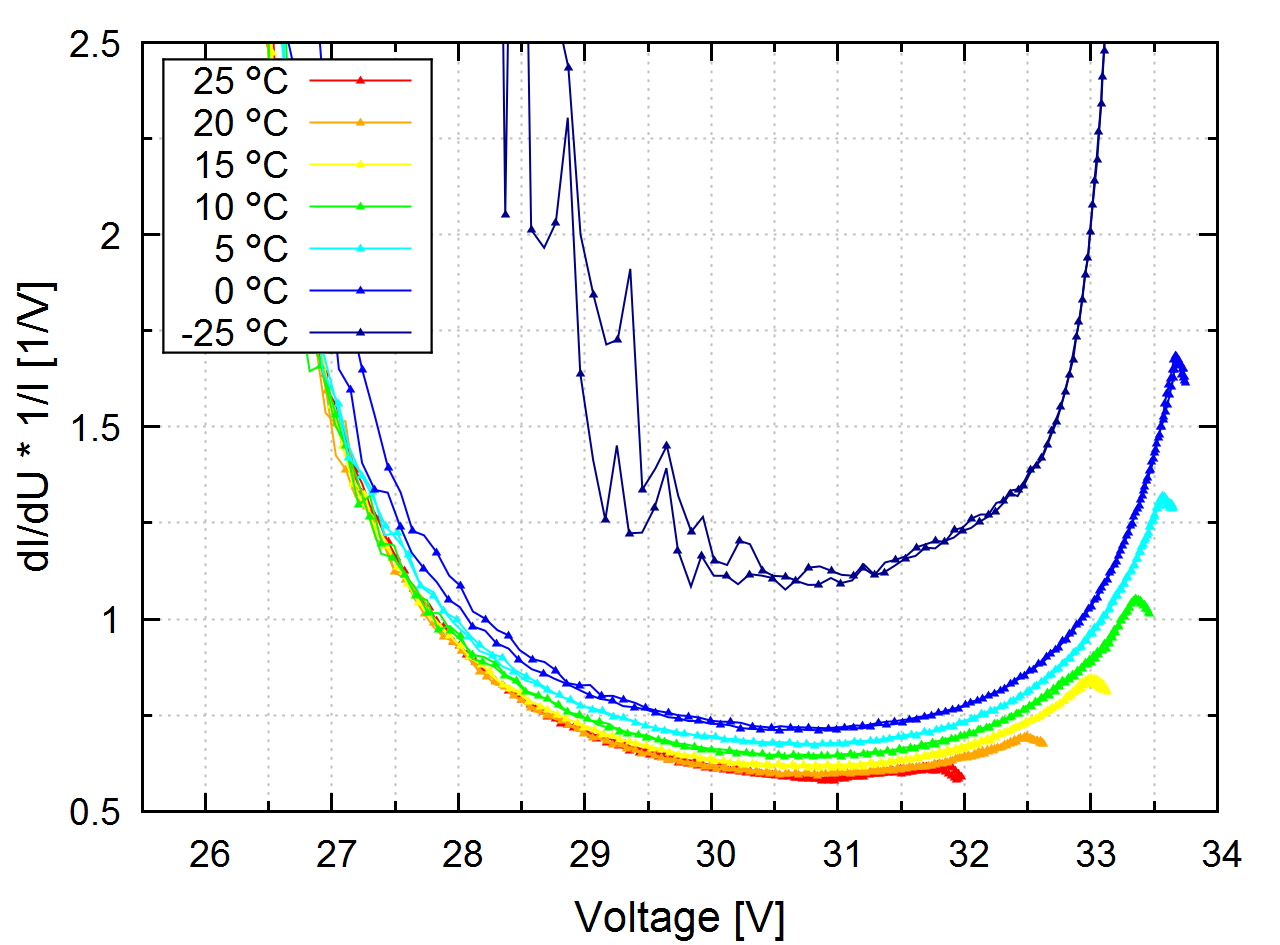
\includegraphics[width=0.49\textwidth]{./plots/iu_curve/1x1n2_op.png}}
	\hfill
	\subfloat[(h)- and (p)-configuration] {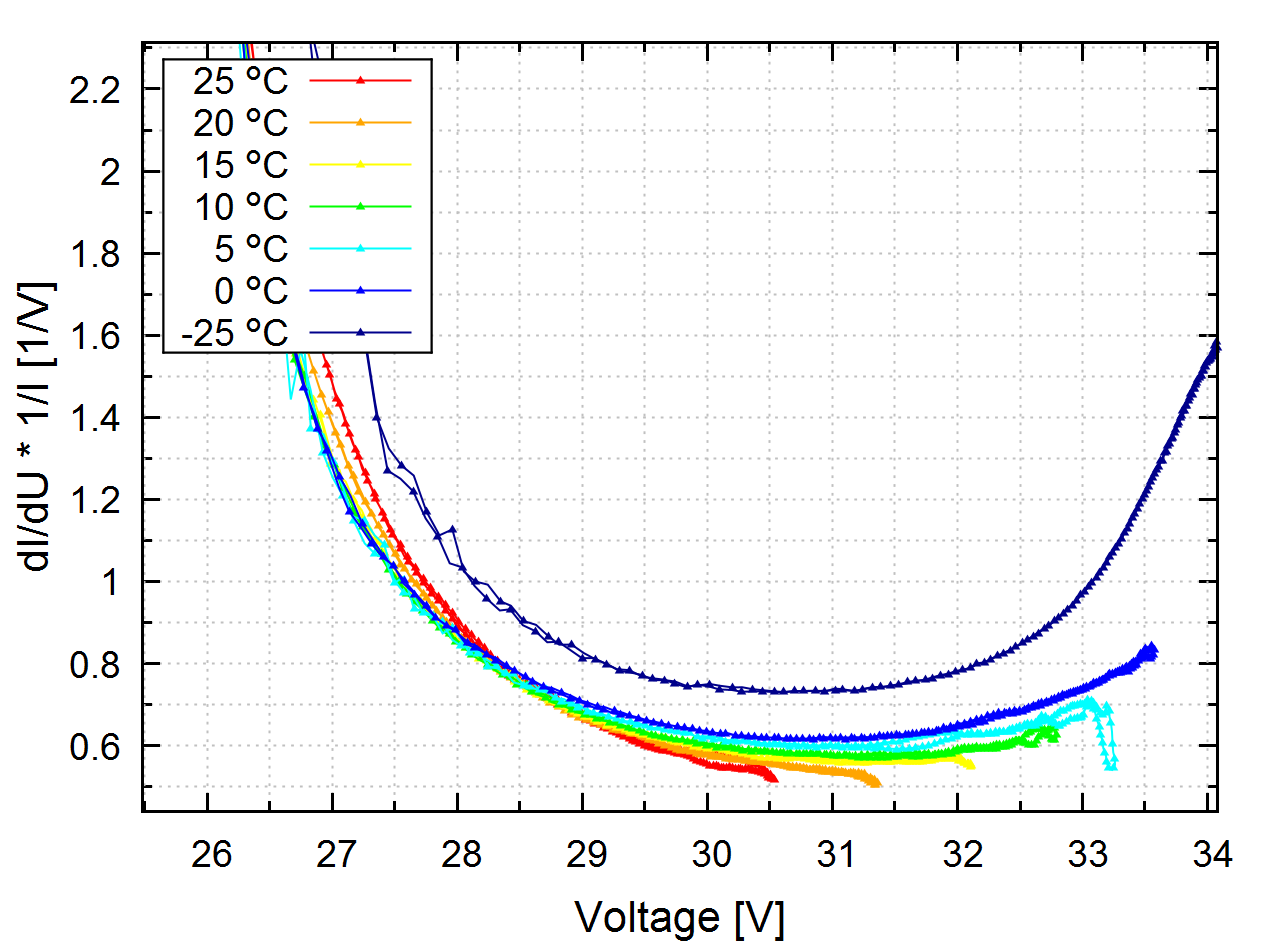
\includegraphics[width=0.49\textwidth]{./plots/iu_curve/4x1n6_op.png}}
	\hfill
	\caption[Comparison of operation voltages]{Comparison of operation voltages. The hybrid and parallel configurations show similar properties.}
	\label{fig:ch4:op_fits}
\end{figure}


The temperature dependence of the breakdown and operation voltages was extracted from the IV-curves. \par 
To calculate the temperature constant $k$, the breakdown voltage was determined. For this, the IV-curves were plotted in logarithmic scale on the y-axis (see \ref{fig:ch4:IV_comparison}). The intersection of a linear fit for the dark current and a second order polynomial fit for the breakdown region provides the sought voltage. The fits can be found in the appendix (see \ref{ap:B:breakdown_fits_single} and \ref{ap:B:breakdown_fits_hybrid}). \par 
\begin{table}[b!]
	\centering
	\begin{tabular}{ c|cc|cc } \toprule[2pt]
		& \multicolumn{2}{c|}{(s)-configuration} & \multicolumn{2}{c}{(h)- and (p)-configuration} \\
		T [$\si{\degreeCelsius}]$ & $V_{OP}$ [$\si{\volt}$] & $V_{BD}$ [$\si{\volt}$] & $V_{OP}$ [$\si{\volt}$] & $V_{BD}$ [$\si{\volt}$]  \\ \midrule
		-25 & $30.78\pm 3.99$ & $24.62\pm 2.89$ & $30.72\pm 0.47$ & $24.40\pm 3.67$ \\
		0 & $30.67\pm 0.42$ & $25.50\pm 0.60$ & $30.89\pm 0.15$ & $24.78\pm 0.03$ \\
		5 & $30.72\pm 0.32$ & $24.93\pm 0.15$ & $31.01\pm 0.59$ & $24.87\pm 0.04$ \\
		10 & $30.70\pm 0.35$ & $25.11\pm 0.44$ & $31.20\pm 0.32$ & $25.04\pm 0.04$ \\
		15 & $30.74\pm 0.28$ & $25.30\pm 0.14$ & $31.32\pm 0.68$ & $25.08\pm 0.01$ \\
		20 & $30.80\pm 0.23$ & $25.35\pm 0.05$ & $31.57\pm 0.75$ & $25.18\pm 0.03$ \\
		25 & $30.87\pm 0.45$ & $25.51\pm 0.23$ & $31.04\pm 2.11$ & $25.20\pm 0.06$ \\
		\midrule
		 & $k_{OP}$ [$\si{\milli\volt\per\kelvin}$] & $k_{BD}$ [$\si{\milli\volt\per\kelvin}$] & $k_{OP}$ [$\si{\milli\volt\per\kelvin}$] & $k_{BD}$ [$\si{\milli\volt\per\kelvin}$]  \\
		 & $6.79\pm 1.34$ & $23.66\pm 5.10$ & $23.67\pm 2.90$ & $19.30\pm 1.51$ \\
		\bottomrule[2pt]
	\end{tabular}
	\caption[Fit results for operation and breakdown voltages]{Fit results for operation and breakdown voltages. Since the same SiPMs were used for (h)- and (p)-configuration the results are the similar.}
	\label{ch4:tab:IV_cata}
\end{table}    
Finding the optimal operation voltage $V_{OP}$ is important for maintaining the detector in the experiment with good a signal-to-noise ratio. One has to trade off high gain and low noise to get sufficient amplification without amplifying too much noise. In order to find this working point, the derivative\footnote{The method for deriving the data is described in \ref{ap:B:sec:derivation}} of the IV-curve has been divided by the current $I(V)$ which results in a local minimum some volts beyond breakdown. The minimum of this relative slope $\dv{I}{V}\frac{1}{I(V)}$ is the voltage where the effect of altering the voltage has the smallest effect in the region beyond breakdown, so small voltage changes should not be as problematic as at other positions. Furthermore, for higher voltages the noise is disproportionately amplified due to high current compared to the amplification of the signal. The minimum was determined by fitting the region with a second order polynomial, again the fits can be found in the appendix (figures \ref{ap:B:optimal_fits_single} and \ref{ap:B:optimal_fits_hybrid}). \par
The results are listed in table \ref{ch4:tab:IV_cata}. The temperature dependence can clearly be seen, the coefficients are positive and and coincide with data provided by KETEK (see data sheet \cite{ketek}). The linear fits are shown in figure \ref{fig:ch4:breakdown_fits}. The (s)-configuration as a single SiPM has a slightly higher $k_{BD}$ with a large error due to difficulties in fitting the $\SI{-25}{\degreeCelsius}$ data (low current).  The operation voltage is roughly $V_{OP}=V_{BD}+\SI{5}{\volt}$ and rises slowly with higher temperature, whereas multiple SiPMs show a steeper slope due to higher intrinsic noise. This suggests to operate the SiPM-boards at $30-31\si{\volt}$ when no precise source is available. Again, the voltage measurement is not calibrated yet, so this is just a rough recommendation. 

 

\begin{figure}[t]
	\subfloat[(s)-configuration] {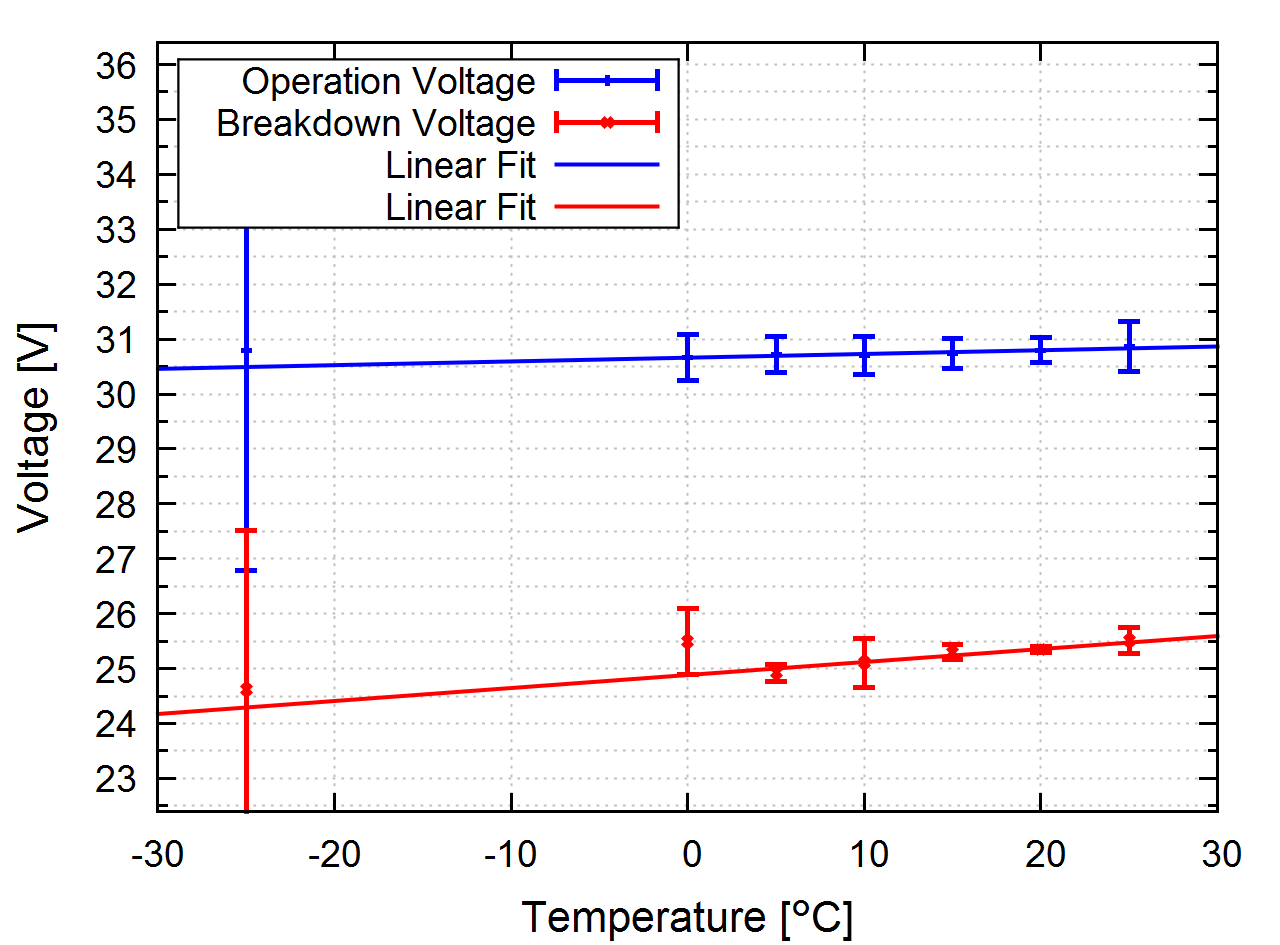
\includegraphics[width=0.49\textwidth]{./plots/iu_curve/1x1n2_fits.png}}
	\hfill
	\subfloat[(h)- and (p)-configuration] {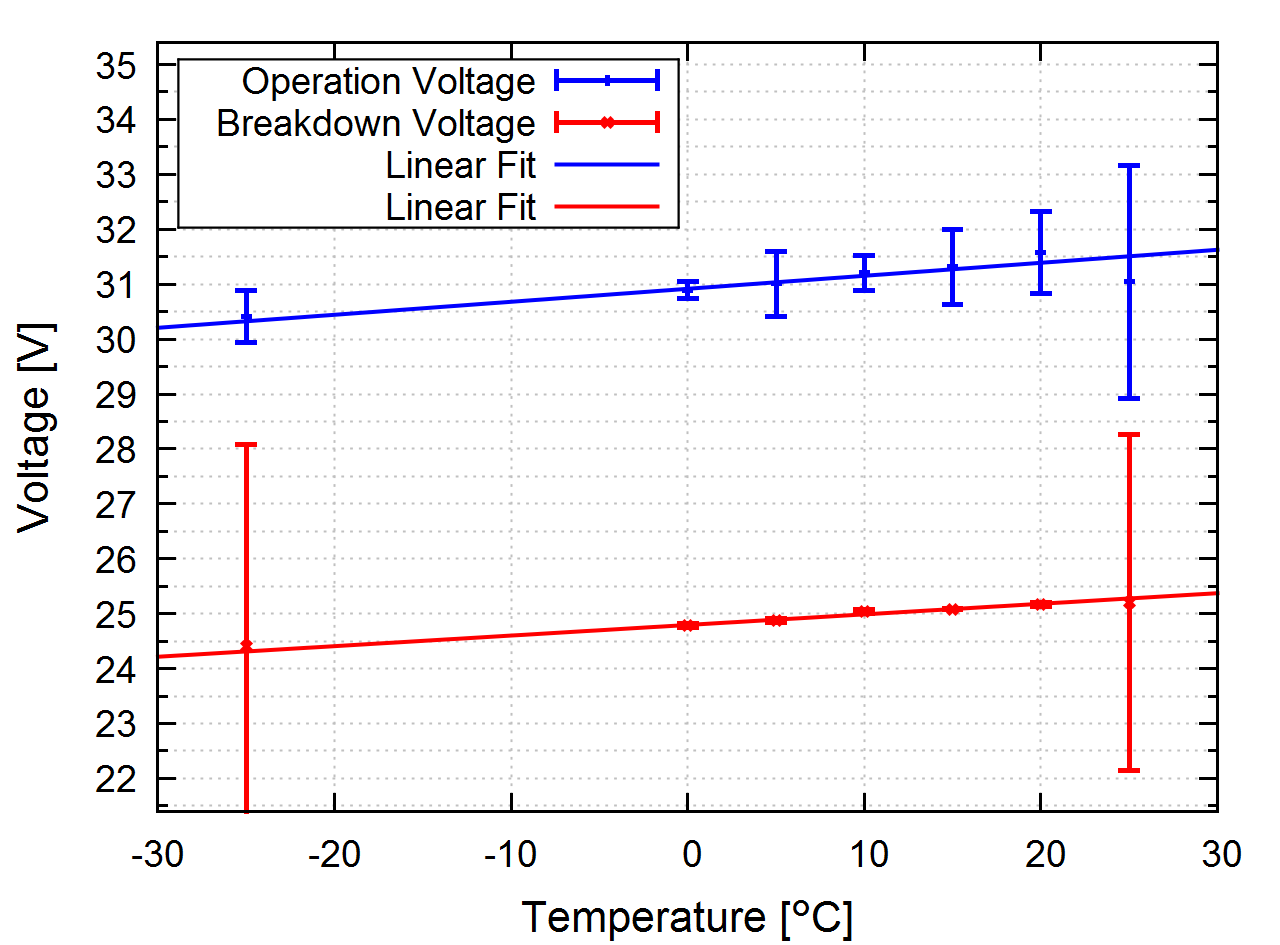
\includegraphics[width=0.49\textwidth]{./plots/iu_curve/4x1n6_fits.png}}
	\hfill
	\caption[Comparison of breakdown and operation voltages]{Comparison of breakdown and operation voltages. The hybrid and parallel configurations show similar properties. Note the positive slope.}
	\label{fig:ch4:breakdown_fits}
\end{figure}


\section{Dark count rate}

Measuring the dark count rate and visualizing the ``dark spectrum" is important for determining a proper threshold level in further experiments when it comes to processing signals right above the noise. \par 
Dark signals are thermally generated signals by electrons with sufficient energy to generate an avalanche. Since the built-in-potential is high, even small thermal energies cause electrons to create avalanches. This results in a high count rate of dark events. \par 
Due to the unique design of the SiPM with discrete micro cell signals, single firing cells contribute most to the count rate. Multiple coincident dark events result in a higher signal whereas the rate for these events is much lower. The probability for a higher number of coincident dark events is close to zero, so the threshold can be set to a level right above a certain number of cells. \par 
\begin{figure}[t]
	\subfloat[(s)-configuration. $\SI{5}{\nano\second}$/div and $\SI{20}{\milli\volt}$/div. Threshold at $\SI{-12}{\milli\volt}$.] {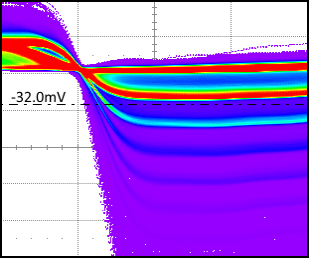
\includegraphics[width=0.475\textwidth]{./plots/darc_electron_spectrum/test16.png}}
	\hfill
	\subfloat[(h)-configuration. $\SI{5}{\nano\second}$/div and $\SI{5}{\milli\volt}$/div. Threshold at $\SI{-8}{\milli\volt}$.] {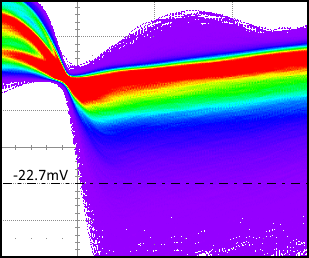
\includegraphics[width=0.475\textwidth]{./plots/darc_electron_spectrum/spectrum_hybrid.png}}
	\hfill
	\caption[Dark spectrum of single and multiple SiPM-configurations]{Dark spectrum of (s)- and (h)-configuration. The single SiPMs shows distinct peaks whereas multiple SiPMs exhibit a more blurred spectrum.}
	\label{fig:ch4:darc_spectrum}
\end{figure}
\begin{figure}[b!]
	\floatbox[{\capbeside\thisfloatsetup{capbesideposition={left,center},capbesidewidth=6cm}}]{figure}[\FBwidth]
	{\caption[Pulse hight spectrum]{Pulse hight spectrum for dark events with single and multiple SiPMs in logarithmic scale and normalized counts per millivolt. The single SiPM shows distinct peaks whereas the spectrum of the hybrid configuration is more blurred and the peaks can only be estimated. }    
		\label{fig:ch4:pulse_hight_hist}}
	{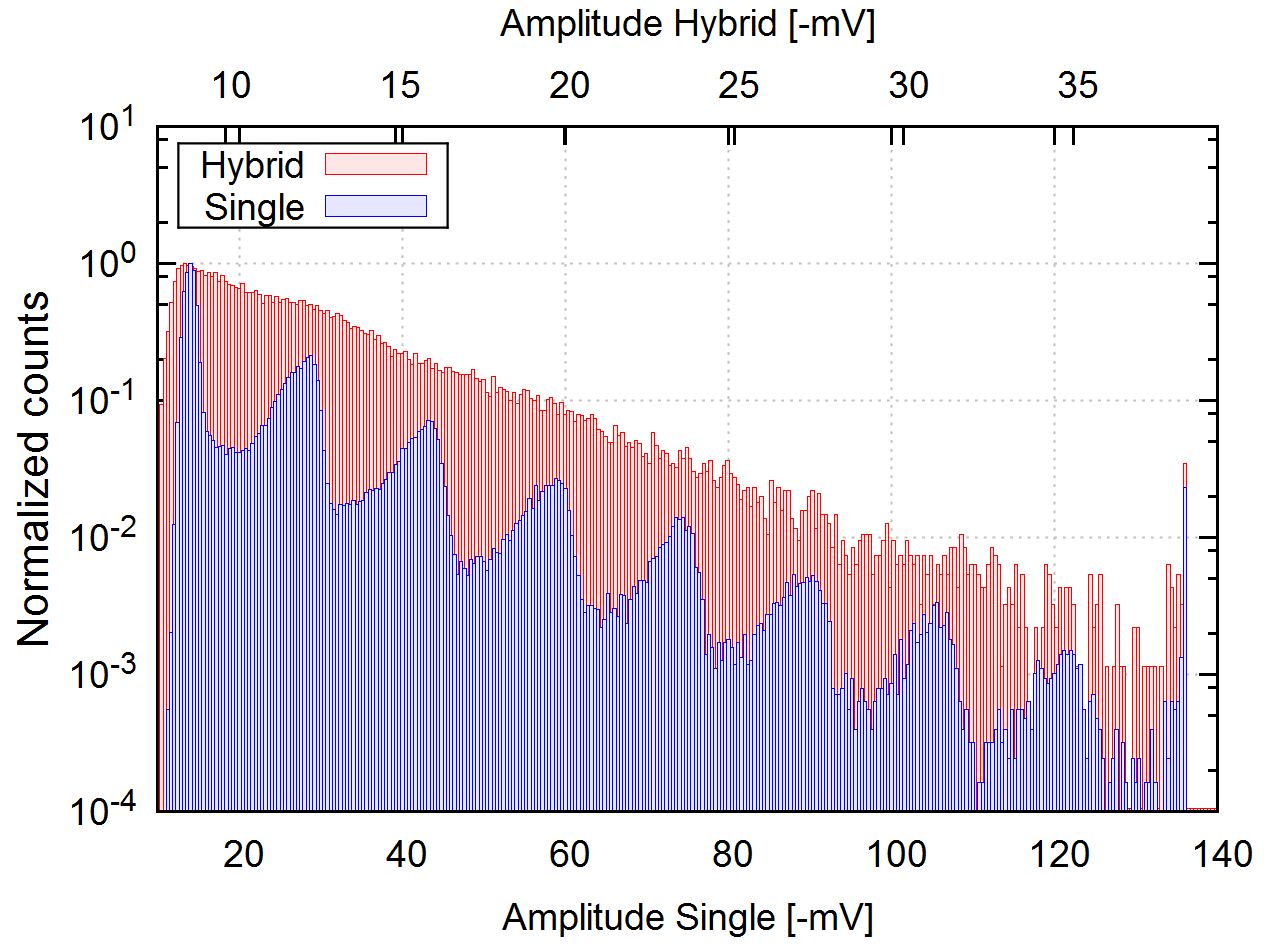
\includegraphics[width=0.6\textwidth]{./plots/darc_electron_spectrum/Counts_multi.png}}
\end{figure}
To get a first qualitative scrutiny of the dark spectrum, a single SiPM and a hybrid board were wrapped light tight with black tape and then stored in a closed aluminum box. The signals were then amplified by a preamplifier in order to get a better resolution of the spectrum. The preamp was operated with $\SI{5}{\volt}$, the SiPM-board with $\SI{30}{\volt}$. The raw signal was tracked and monitored by a \tit{LeCroy Waverunner 104MXi-A 1GHz} oscilloscope. \par 
With persistence setup, a waveform-picture of more than 10.000 signals was taken for both configurations which can be seen in figure \ref{fig:ch4:darc_spectrum}. The single SiPM shows distinct peaks, the discrete signal height for a single cell can be roughly estimated as \SI{15}{\milli\volt}. The spectrum of multiple SiPMs is more blurred due to slightly different characteristics of each SiPM in the array. Still, a stepwise distribution of signals can be observed which also can be used to estimate the number of firing cells. \par  
This can be represented distinctly by plotting the pulse height. The histogram \ref{fig:ch4:pulse_hight_hist} visualizes the counts per millivolt in logarithmic scale and normalized count rate per millivolt. The single SiPM shows distinct peaks with a gap of roughly \SI{15}{\milli\volt}, the spectrum of multiple SiPMs is blurred and the steps are not as distinct as for a single SiPM. \par 
\begin{figure}[t]
	\centering
	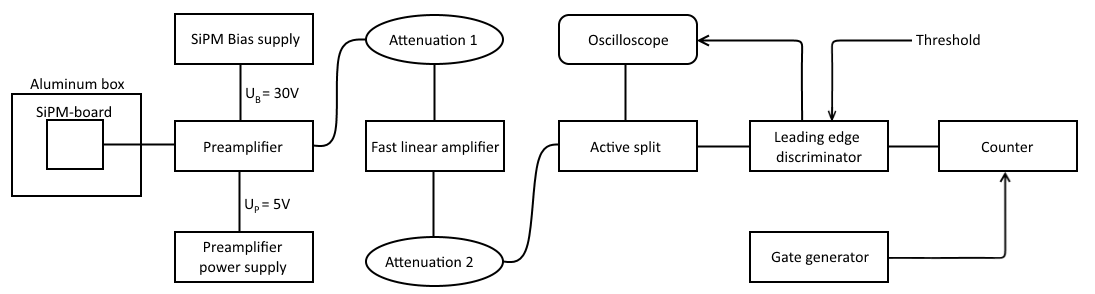
\includegraphics[width=1\linewidth]{./graphics/ch4/scheme_count_rate.png}
	\caption[Schematic of the dark count rate measurement]{Schematic of the dark count rate measurement.}
	\label{fig:ch4:scheme_rate}
\end{figure}
\begin{figure}[b]
	\floatbox[{\capbeside\thisfloatsetup{capbesideposition={right,center},capbesidewidth=0.4\linewidth}}]{figure}[\FBwidth]
	{\caption[Slope of the dark count rate]{Normalized slope of dark count rate. The single SiPM (blue) shows distinct steps whereas the other configurations do not show such a behavior.}    
		\label{fig:ch4:slope_countrate}}
	{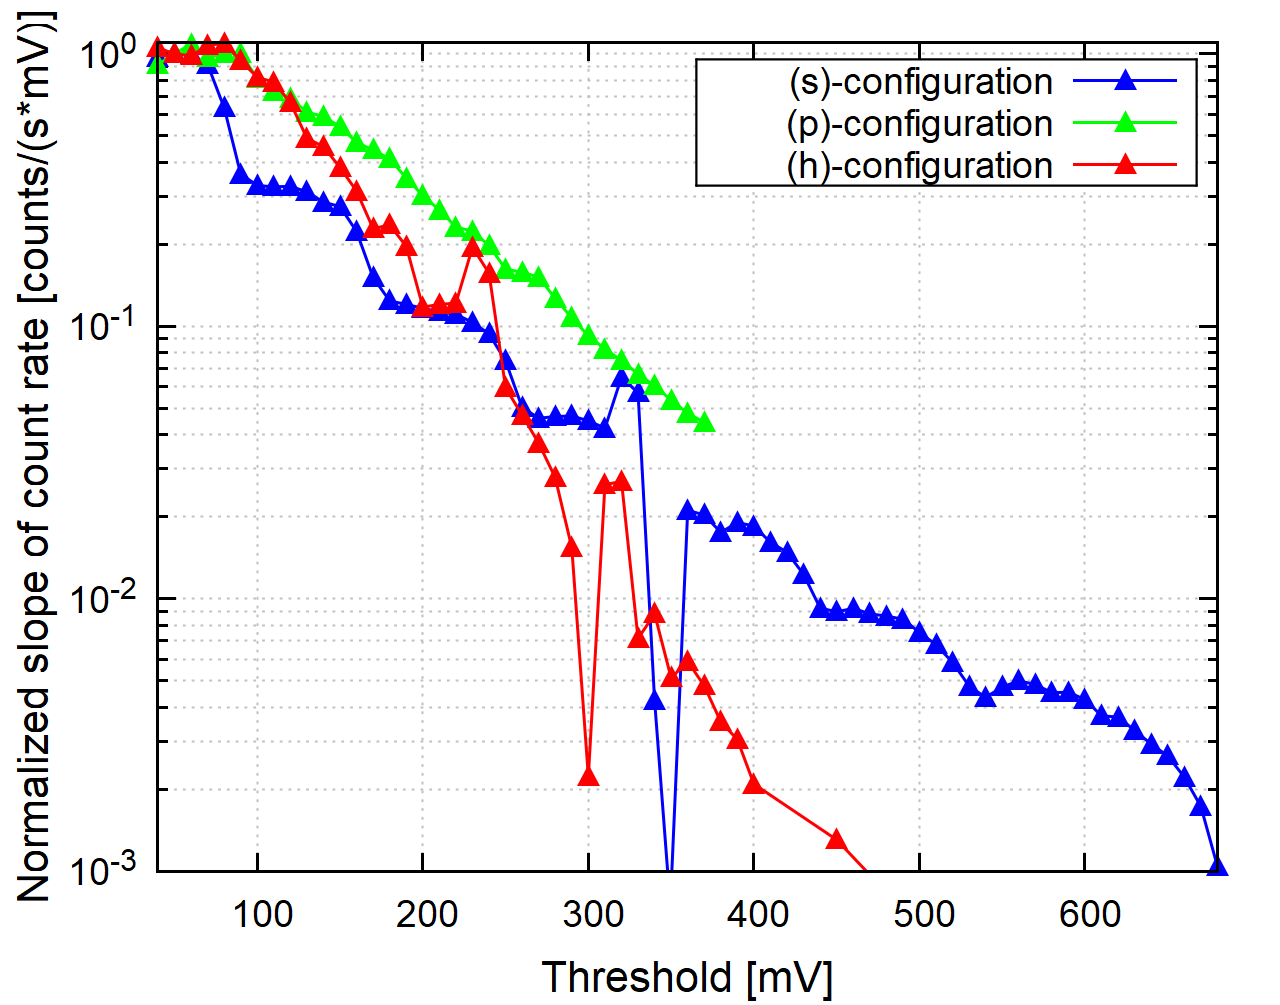
\includegraphics[width=0.6\textwidth]{./plots/darc_electron_spectrum/slope_countrate.png}}
\end{figure}
To measure the count rate of the different configurations, the setup shown in figure \ref{fig:ch4:scheme_rate} was used. Again, the SiPM-boards were wrapped light tight, stored in the aluminum box and operated by the preamplifier. To exploit the whole range of the available leading edge discriminator (Lecroy 623B, threshold $\SI{-30}{\milli\volt}$ to $\SI{-800}{\milli\volt}$), some further amplifications had to be made. A fast linear amplifier (FTA810L from GSI, V=800, $\tau\leq\SI{10}{\nano\second}$) was used for this reason, but to avoid saturation of this amplifier and to further fine tune the signal range, passive attenuators were utilized before and after the amplifier. An active split divided the signal for monitoring the threshold level of the discriminator. A megahertz counter (from Uni Bonn) was gated by a gate generator (Lecroy 222) to count the signals for $\SI{10}{\second}$. \par 
The first derivative was calculated\footnote{Again, the method used is described in \ref{ap:B:sec:derivation}} from the retrieved data to emphasize the expected drop in count rate. Figure \ref{fig:ch4:slope_countrate} shows this normalized slope of count rate in logarithmic scale. The single SiPM (blue) yields the unique stepwise drop in count rate with a width of approximately $\SI{80}{\milli\volt}$ per step. Again, the array configurations do not show such a distinct behavior. \par 
The absolute count rate and slope of each setup for prominent threshold levels is given in table \ref{ch4:tab:count_rate}, note that the edges of the first five steps of the single SiPM are used for highlighting the discrete spectrum. This behavior could not be found in the array setups, the slope is nearly linear which indicates a exponential decrease in count rate. \par 

\begin{table}[t]
	\centering
	\begin{tabular}{ c|cc|cc|cc } \toprule[2pt]
		& \multicolumn{2}{c|}{(s)-configuration} & \multicolumn{2}{c|}{(h)-configuration} & \multicolumn{2}{c}{(p)-configuration} \\
		TH [$\si{\milli\volt}]$ & $f$ [$\si{\kilo\hertz}$] & Slope [$\si{\kilo\hertz\per\volt}$] & $f$ [$\si{\kilo\hertz}$] & Slope [$\si{\kilo\hertz\per\volt}$] & $f$ [$\si{\kilo\hertz}$] & Slope [$\si{\kilo\hertz\per\volt}$] \\ \midrule
		-30 & 1827 & 190 & 4089 & 360 & 3389 & 300 \\
		-80 & 866 & 180 & 2335 & 400 & 2274 & 200 \\ \midrule
		-90 & 786 & 60 & 2006 & 330 & 2024 & 225 \\
		-160 & 355 & 60 & 603 & 110 & 963 & 110 \\ \midrule
		-170 & 319 & 20 & 508 & 100 & 859 & 100 \\
		-250 & 141 & 19 & 87.6 & 23 & 340 & 40 \\ \midrule
		-260 & 121 & 10 & 70.9 & 17 & 304 & 35 \\
		-340 & 50.9 & 9.0 & 13.7 & 5.0 & 119 & 14 \\ \midrule
		-350 & 48.9 & 2.9 & 12.4 & 1.3 & 107 & 12.5 \\
		-430 & 27.6 & 3.0 & 1.77 & 0.2 & $-$ & $-$ \\ \midrule
		-440 & 25.6 & 1.9 & $-$ & $-$ &  $-$ &  $-$ \\
		-500 & 15.1 & 1.6 & $-$ &  $-$ &  $-$ &  $-$ \\
		-600 & 4.8 & 0.7 & $-$ & $-$ &  $-$ &  $-$ \\
		-720 & 0 & 0 & $-$ & $-$ &  $-$ &  $-$ \\
		\bottomrule[2pt]
	\end{tabular}
	\caption[Absolute dark count rate]{Absolute dark count rate for different configurations. The steps (drop in count rate) for the single SiPM are highlighted by horizontal lines.}
	\label{ch4:tab:count_rate}
\end{table}  

For the single SiPM, the rate has been measured until no counts were registered within $\SI{10}{\second}$. This point is reached at $\SI{-720}{\milli\volt}$. The data indicates steps with a width of $\SI{80}{\milli\volt}$, so the upper limit for coincident firing cells is nine cells at the same time. The rate for single cells lies in the megahertz region, for five cells in the low kilohertz region, for seven cells some hundreds of hertz. The rate for the array setups is nearly four times the rate of a single cell. \par 
Further work on comparing pulse signals, timing response and energy measurements will be shown in chapter \ref{ch:timing}, in which the different configurations were mounted to a plastic scintillator of type \tit{EJ-248M} from \tit{ELJEN} and inorganic crystals, LYSO and \pwo{}.











\chapter{Time and energy measurements} \label{ch:timing}
Substituting photomultiplier tubes or avalanche photodiodes with SiPMs in some applications could be a possible way to save space, funds, and avert the dependence on high voltage power supplies. Some of these applications, i.e. timing and energy measurements, were tested by mounting different SiPM-boards to plastics and crystals.     
\section{Signal shaping} \label{ch5:signal_shaping}
\begin{figure}[b!]
	\subfloat[Single SiPM with mask and optical grease] {\includegraphics[width=0.4\textwidth]{./pictures/plastic/SiPM_grease.jpg}}
	\hfill
	\subfloat[Mounted SiPM-boards on the plastic scintillator] {\includegraphics[width=0.4\textwidth]{./pictures/plastic/plastic_measurement.jpg}}
	\hfill
	\caption[Plastic scintillator measurement]{Mechanical setup for the efficiency and timing measurement with a plastic scintillator (wrapped, with graph paper) and \sr{} source (blue bar). A schematic can be found in figure \ref{fig:ch5:scheme_counting}.}
	\label{pic:ch5:plastic}
\end{figure}
The dark count rate measurements showed that the signal response is different for the board configurations. To obtain more information about the actual signal shape, the three configurations were mounted consecutively on opposing sides of a $\SI{25.50}{\centi\meter}\times\SI{12.25}{\centi\meter}$ plastic scintillator plate \tit{EJ-248M} from \tit{ELJEN} (see table \ref{ch2:tab:characteristics}) with cut edges and a thickness of $\SI{10}{\milli\meter}$ (a detailed schematic can be found in \ref{ap:C:plastic}). This design was chosen for measuring cosmic muons for the project \tit{Cosmic Radiation: Measuring Cosmic Muons with the Raspberry Pi} \cite{schauer_projekt}, because this shape provides a large area with a ``pseudo" light-guide to the more narrow edges where the SiPM boards will be attached.\par   
The plastic detector was wrapped with eight layers of Teflon foil and then covered with opaque black foil. For mounting, the SiPM boards were equipped with a thick rubber mask to fill the spacing between the diodes. Onto this mask a reflective foil was attached. Optical grease was carefully spread over each SiPM to grant good optical coupling with the scintillator material. The connection between board and plastic was fixed with black tape, an electrical connection was established via a pin header for the cathode and anode contacts. This setup can be see in figure \ref{pic:ch5:plastic}, a schematic is shown in figure \ref{fig:ch5:scheme_counting}, for more pictures see appendix \ref{ap:C:pictures}. A ``Bias T" was built for reading out the raw signal (see figure \ref{fig:ch5:bias_t}).  \par
\begin{figure}[t!]
	\floatbox[{\capbeside\thisfloatsetup{capbesideposition={left,center},capbesidewidth=0.65\linewidth}}]{figure}[\FBwidth]
	{\caption[``Bias T"]{``Bias T" for reading out the raw signal. The bias voltage (DC) is applied between anode (positive) and cathode (ground) for reverse biasing. A series resistor $R=\SI{10}{\kilo\ohm}$ is placed between anode and power supply, a capacitor $C=\SI{100}{\nano\farad}$ is placed between resistor and signal output and decouples the AC signal of the SiPM from the DC biasing   }    
		\label{fig:ch5:bias_t}}
	{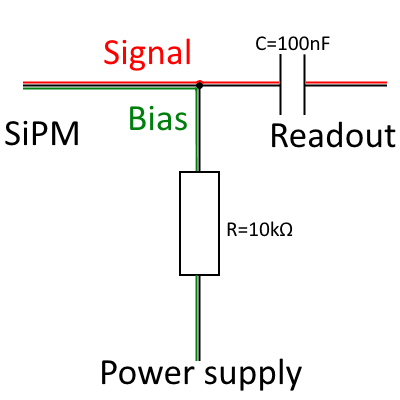
\includegraphics[width=0.3\textwidth]{./graphics/ch5/biast.png}}
\end{figure}
\begin{figure}[b!]
	\subfloat[Raw signal of the different configurations: blue (4x1 hybrid), red (4x1 parallel), green (1x1 single)] {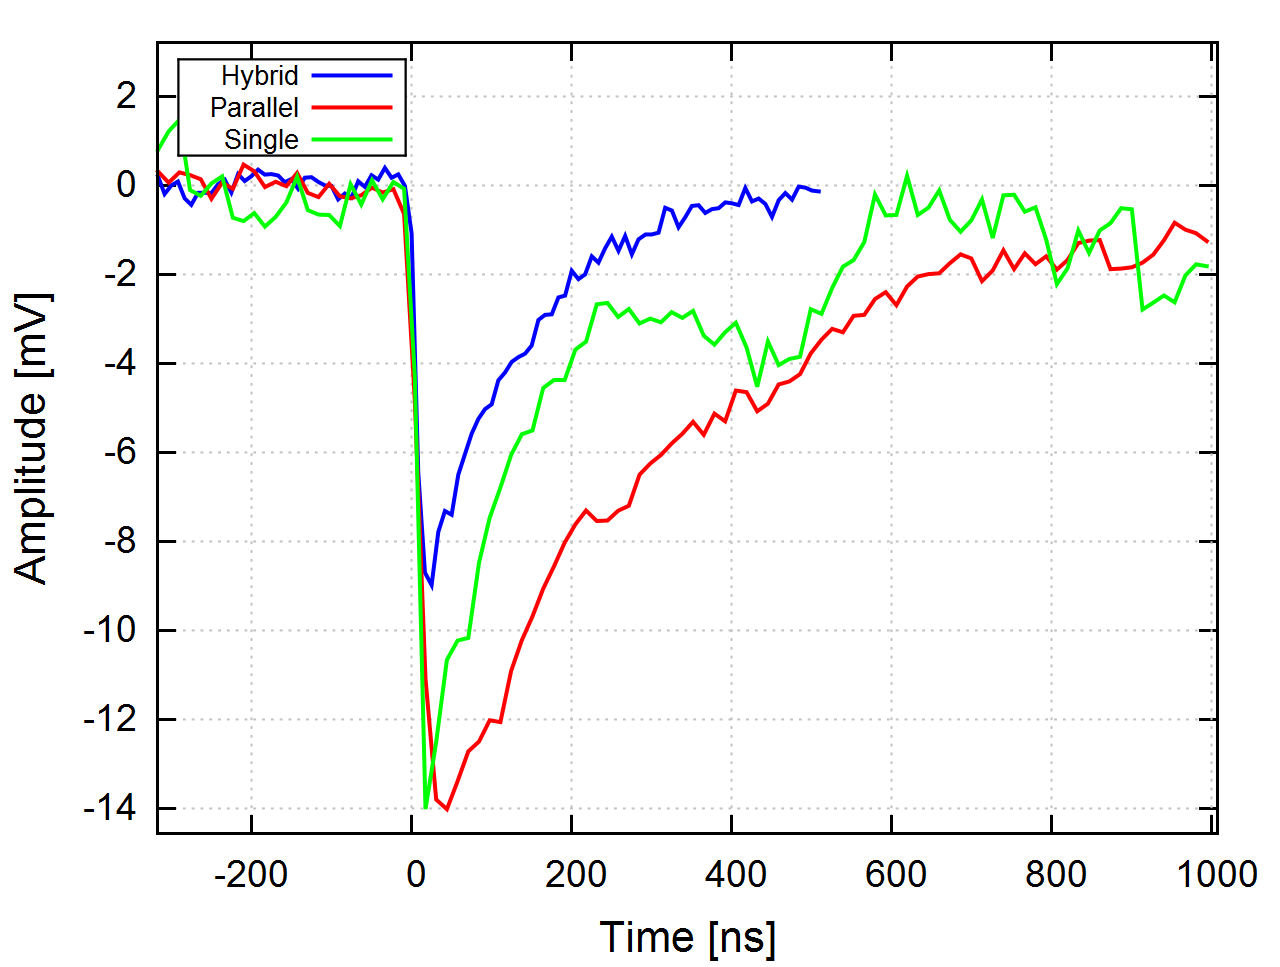
\includegraphics[width=0.49\textwidth]{./plots/signal/raw.png}}
	\hfill
	\subfloat[Amplified signal of blue (4x1 hybrid), red (4x1 parallel), green (1x1 single) with utilized photonique preamplifier] {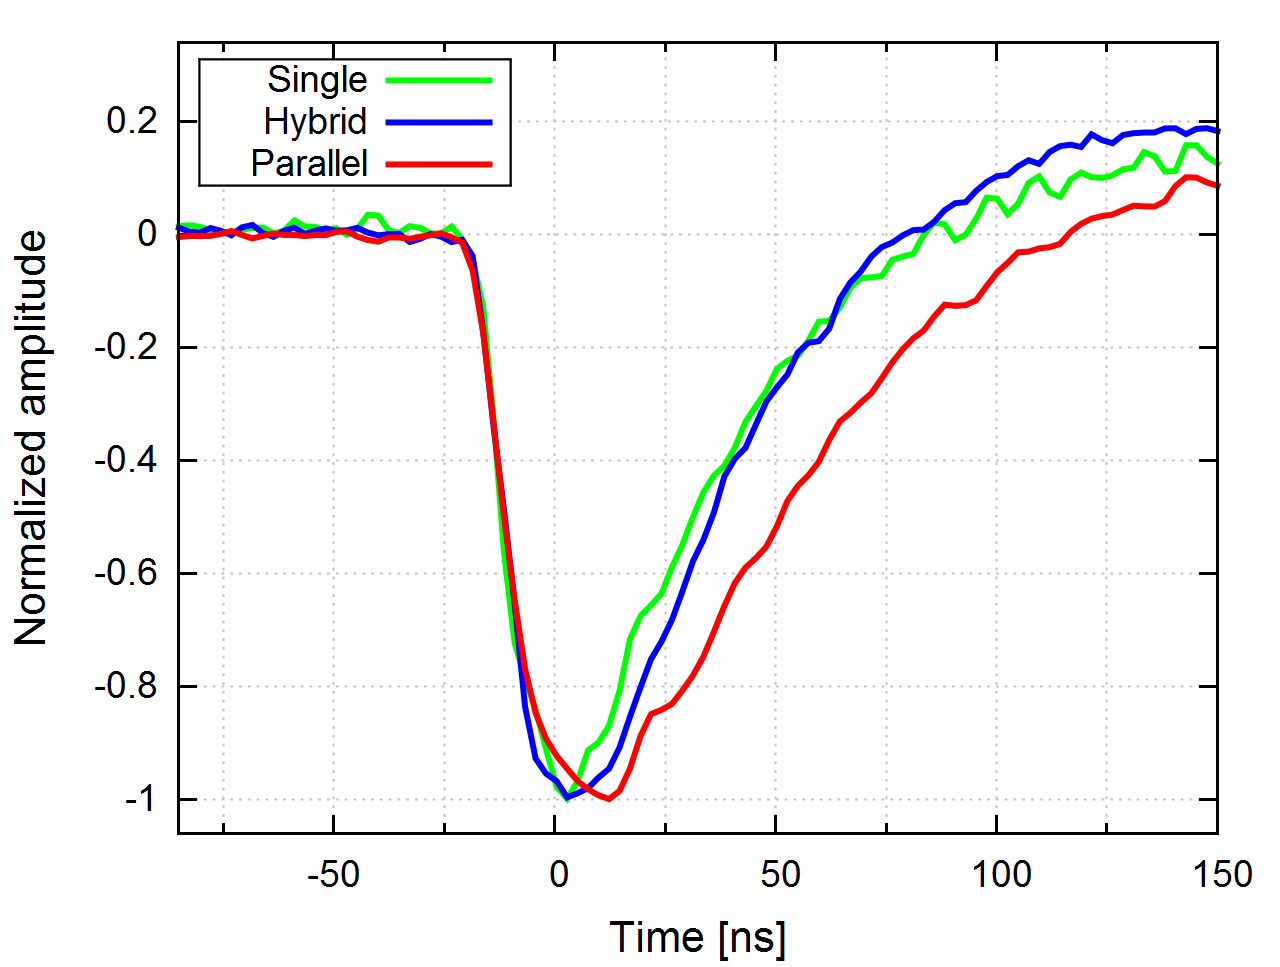
\includegraphics[width=0.49\textwidth]{./plots/signal/amp.png}}
	\hfill
	\caption[Signal shaping]{Raw and amplified signals of different SiPM configurations.}
	\label{fig:ch5:signals}
\end{figure}
With the oscilloscope used before (\tit{LeCroy Waverunner}), waveforms of the raw signals of the different SiPM configurations were acquired. For this, the SiPMs were powered with a four-channel bias source from \tit{Hameg} via the ``Bias T", the signals were fed directly to the oscilloscope. For measuring the amplified signals, the Bias T's were substituted with the \tit{photonique} preamplifiers. It was observed, that the connection between SiPM-board and preamplifier had to be as short as possible to avoid ringing and an increased noise. This was solved by directly connecting the preamp via a pin header. The bias voltage was set to $U_B=\SI{30}{\volt}$ and the power supply for the preamps was set to $U_P=\SI{5}{\volt}$. The pictures can be seen in figure \ref{fig:ch5:signals}. 
It appears that the signal amplitude of the single and parallel configurations are nearly equal, whereas the amplitude of the hybrid board is roughly half in size. Also, the baseline noise for the hybrid and parallel configurations seem to be less fluctuating. The signal rise time, which is in order of some nanoseconds, can be compared by normalizing the pulse height: the parallel configuration shows the longest rise time, the hybrid configuration the fastest. The single SiPM lies right in between. For timing, the hybrid configuration might be the most valid candidate. Even better timing can be achieved by driving the SiPMs in series, done by the PANDA Barrel-TOF detector \cite{SciTil}, but this necessitates $N$ times the bias voltage of a single SiPM, where $N$ is the number of SiPMs in series. This configuration is not considered in this thesis because of its necessity of using high voltage.   


\section{Efficiency measurements}
As a preparation for the upcoming timing measurement, the efficiency of the setup with the thin plastic scintillator plate was measured. The investigations undertaken in the last section confirmed that the hybrid configuration has the fastest rise time, so two hybrid boards were mounted to the scintillator plate used before.
\begin{figure}[b]
	\centering
	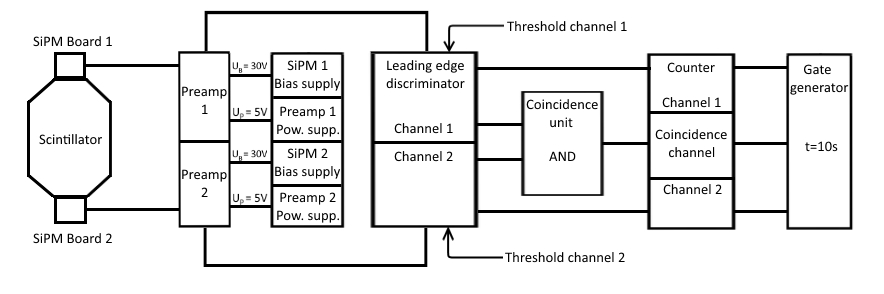
\includegraphics[width=1\linewidth]{./graphics/ch5/scheme_spatial.png}
	\caption[Schematic of the efficiency measurement]{Setup of the efficiency measurement.}
	\label{fig:ch5:scheme_counting}
\end{figure}
The experimental setup can be seen in figure \ref{fig:ch5:scheme_counting}: a four-channel power supply (Hameg HMP4040) biases the two hybrid boards with $U_{B}=\SI{30}{\volt}$ and the photonique preamplifiers with $U_{P}=\SI{5}{\volt}$. The amplified signals of the channels one and two were then discriminated by a leading edge discriminator (Lecroy 623B, TH$_1=\SI{-450}{\milli\volt}$, TH$_2=\SI{-477}{\milli\volt}$), the threshold levels TH were set to satisfy the expected count rate of cosmic muons (approximately $\SI{200}{\per\second\per\meter\squared}$ \cite{PDG}). The output of the discriminator was tracked by a counter (Uni Bonn) which was gated by a gate generator (Lecroy 222) to count the signals for $\SI{10}{\second}$. A coincidence unit (Caen N455) provided the signal to count coincident signals. \par 
A \sr{} source ($\beta^{-}$-emitter) was used to produce scintillation light. An aluminum block with a small bore was used as a collimator to guide and center the emitted electrons. For positioning, graph paper was attached to the scintillator (again, see \ref{pic:ch5:plastic}). \par
The measurement positions are show in figure \ref{fig:ch5:efficiency}. The heat map plots for the count rate show two maxima: one right in front of the SiPMs, the other on the y-axis some centimeters in front of the detectors, beginning half the way down from the center of the scintillator to the mounted boards. This region of high count rate is limited to some square centimeters and is oval shaped. The count rate in the other regions of the plastic is nearly constant, except from the very edges and corners, and right in front of the respective opposite detector, where the rate drops. The results for detector one and two are similar but not identical: detector one seems to be less effective in counting compared to detector two, which shows a more symmetric shape. The second maximum might be explained by the special shape of the cut corners, so the photons generated at this position might get reflected to the detectors. \par 
In discussing the coincident count rate, the asymmetry can be found again: the rate right in front of detector two is nearly twice as high as in front of detector one. The maxima appear again at the same positions, the rate is highest on the y-axis and decreases for positions moving along the x-axis. For events right in front of one board, the coincident count rate is apparently given by the count rate of the opposite board. \par 
Although one of the two detectors seems to have some performance issues, the coincident count rate for most of the positions, a square from -5$\si{\centi\meter}$ to +5$\si{\centi\meter}$ on the x-axis and -9$\si{\centi\meter}$ to +9$\si{\centi\meter}$ on the y-axis, is valid for using this setup for measuring cosmic muons (two detectors are used to avert detecting fake events). The time resolution will be discussed in the section following.

\section{Time resolution measurements}

For certain applications like propagation time measurements or positioning, timing properties are important. As section \ref{ch5:signal_shaping} has shown, the hybrid configuration is a valid candidate for timing applications. The time resolution and propagation time was measured for the setup used in last section. \par 
\begin{figure}[h!]
	\subfloat[Measurement positions] {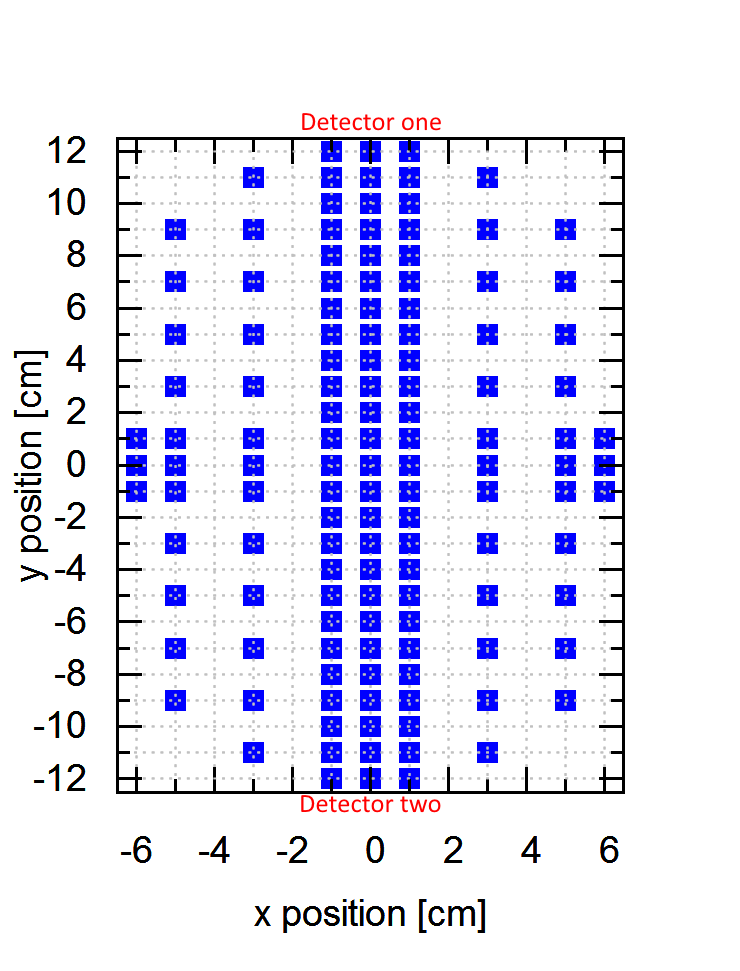
\includegraphics[width=0.4\textwidth]{./plots/spatial/aufnahme_punkte.png}}
	\hfill
	\subfloat[Detector one] {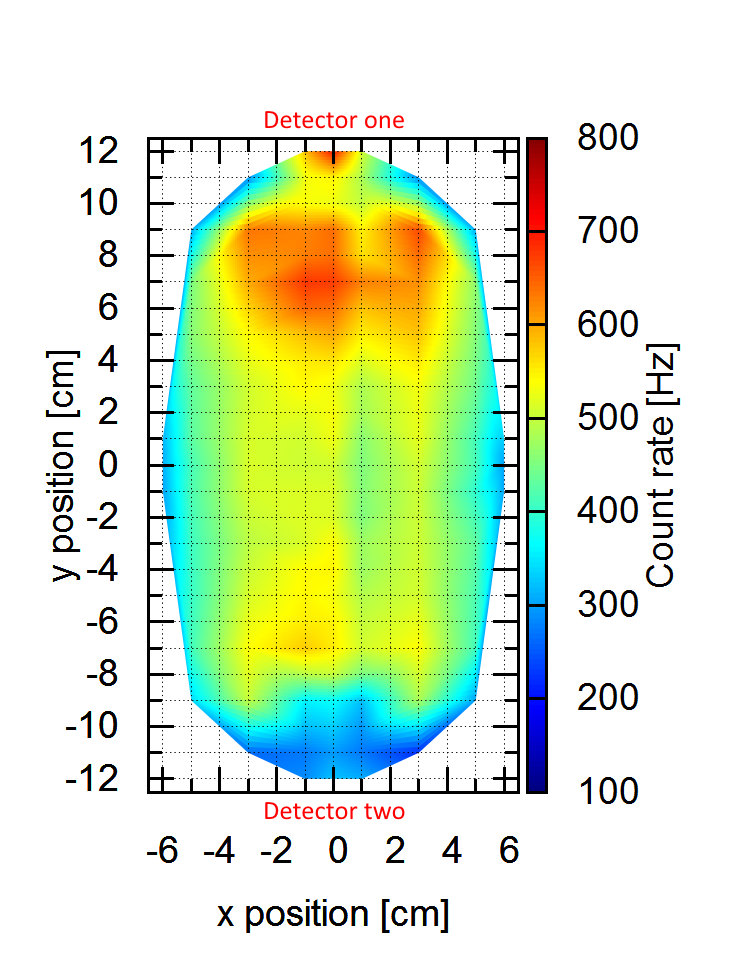
\includegraphics[width=0.4\textwidth]{./plots/spatial/Det1.png}}
	\hfill
	\subfloat[Detector two] {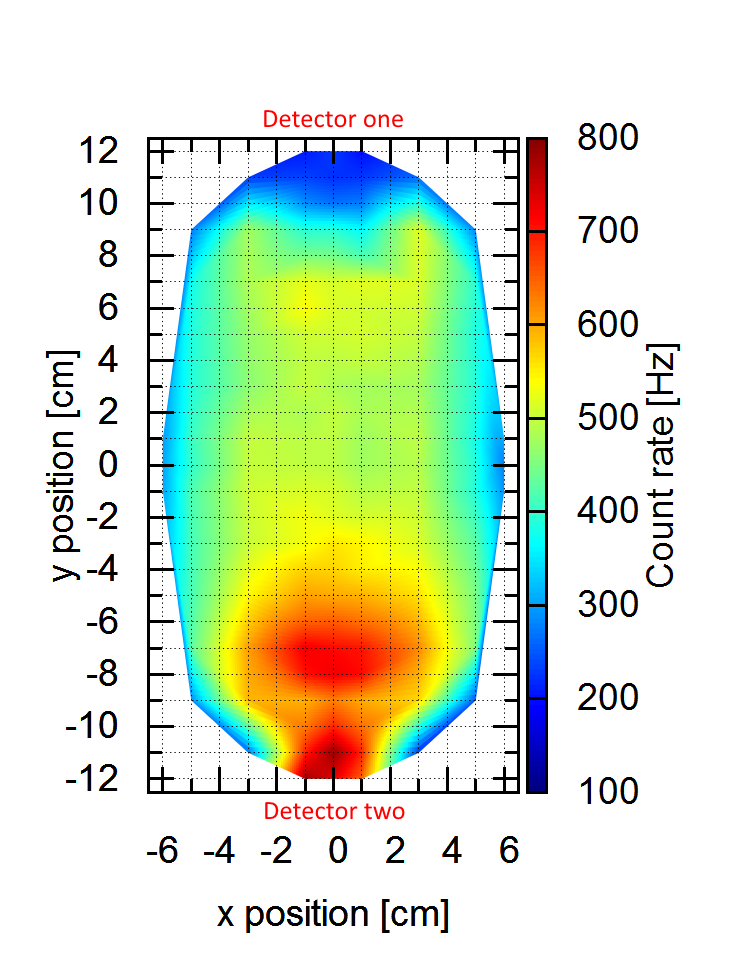
\includegraphics[width=0.4\textwidth]{./plots/spatial/Det2.png}}
	\hfill
	\subfloat[Coincidence rate] {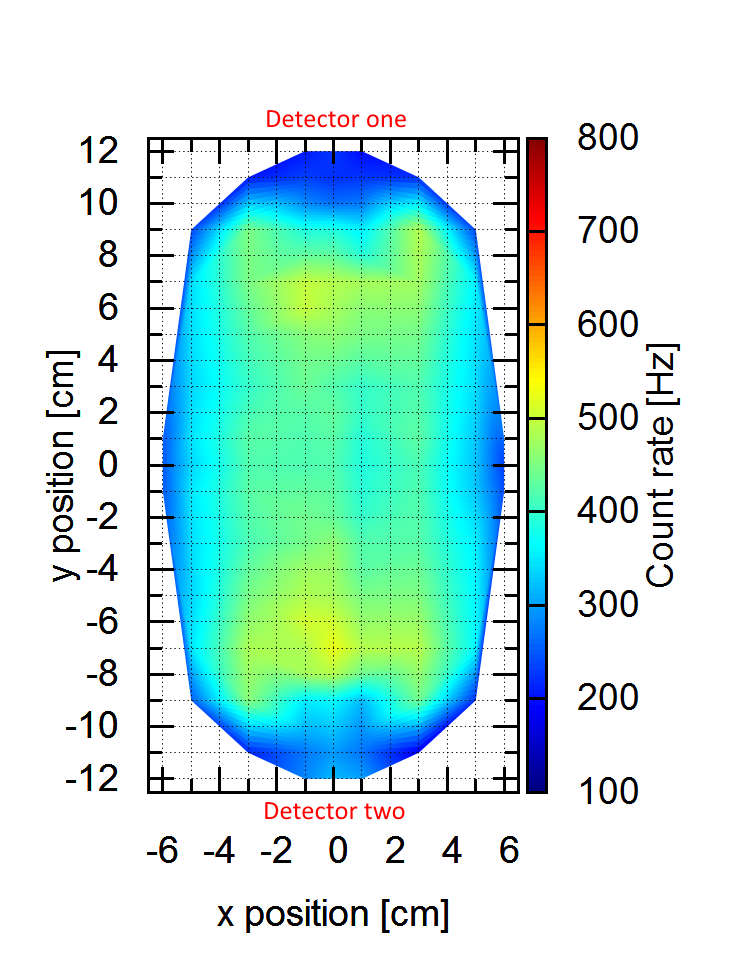
\includegraphics[width=0.4\textwidth]{./plots/spatial/Coinc.png}}
	\hfill
	\caption[Efficiency measurement setup]{Efficiency measurement at plastic scintillator with a \sr{} source at different positions. The heat map was plotted with \tit{gnuplot's pm3d} feature, the data between the measurement points was interpolated by the same software. Note that the coincidence count rate in front of one detector is mainly dominated by the count rate of the opposite detector.}
	\label{fig:ch5:efficiency}
\end{figure} 
\newpage
Nevertheless, the readout setup had to be changed to avoid walk (see figure \ref{fig:ch5:scheme_timing}). To do so, the leading edge discriminator was replaced by a \tit{constant fraction discriminator} (CF4000 from GSI, $\SI{1}{\nano\second}$ delay line, adjustable threshold and zero cancellation). Furthermore, a \tit{time to pulse height converter} (Ortec 437A) was installed to display the time differences between detector one and two as a pulse height. This necessitates signal one (start) to be definitely earlier than signal two (stop), so signal two was delayed with a constant delay (long cable, $\SI{50}{\nano\second}$). To avoid noise in the time spectrum, the coincident signal of one and two gated the TPC in order to just register events, in which the signals are coincident. The pulse height spectrum was digitized by a $13$-bit \tit{analog-to-digital converter} (Caen N957) and monitored by a \texttt{root}\footnote{\texttt{root}: data analysis framework by CERN \cite{root}} framework on a UNIX-system. \par
\begin{figure}[t!]
	\centering
	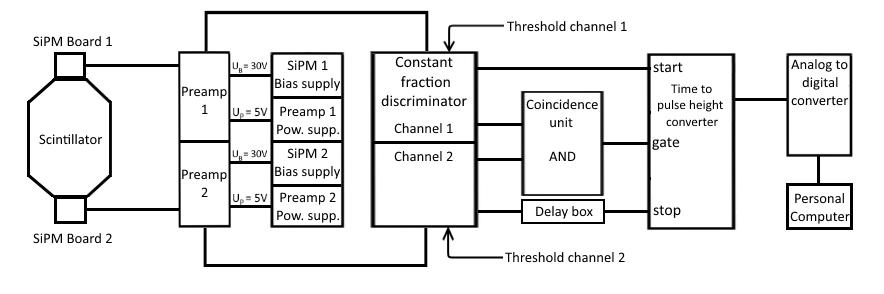
\includegraphics[width=1\linewidth]{./graphics/ch5/scheme_timing.png}
	\caption[Schematic of the time resolution measurement]{Setup of the time resolution measurement.}
	\label{fig:ch5:scheme_timing}
\end{figure} 
\begin{figure}[b!]
	\centering
	\subfloat[Time calibration spectrum. The second x-axis already shows the calibrated time. The key represents the employed delays.] {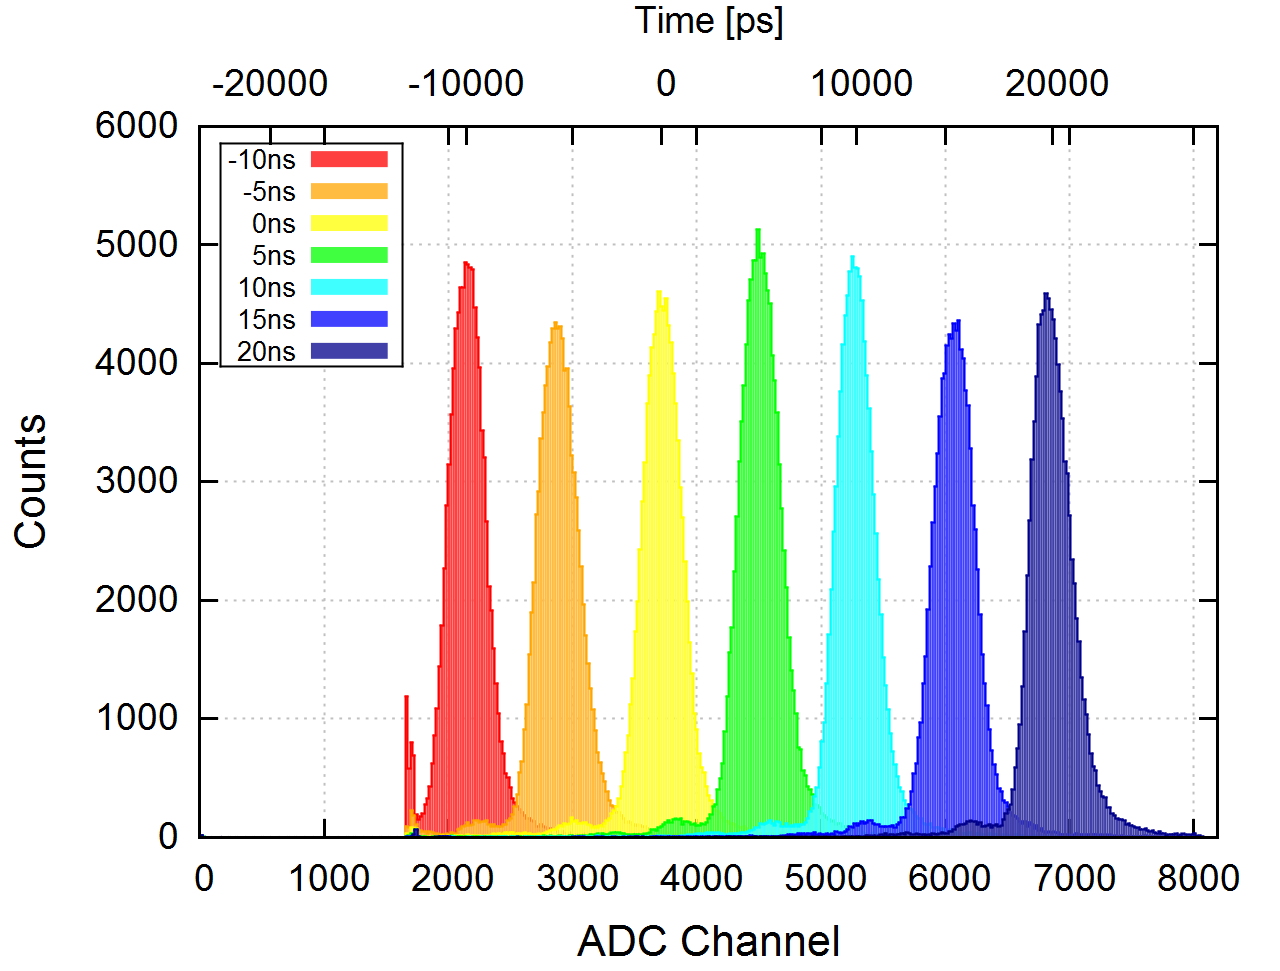
\includegraphics[width=0.49\textwidth]{./plots/timing/ze_hist.png}}
	\hfill
	\subfloat[Time calibration fit. The datapoints were extracted via Gaussian fits, using the \texttt{root} framework.] {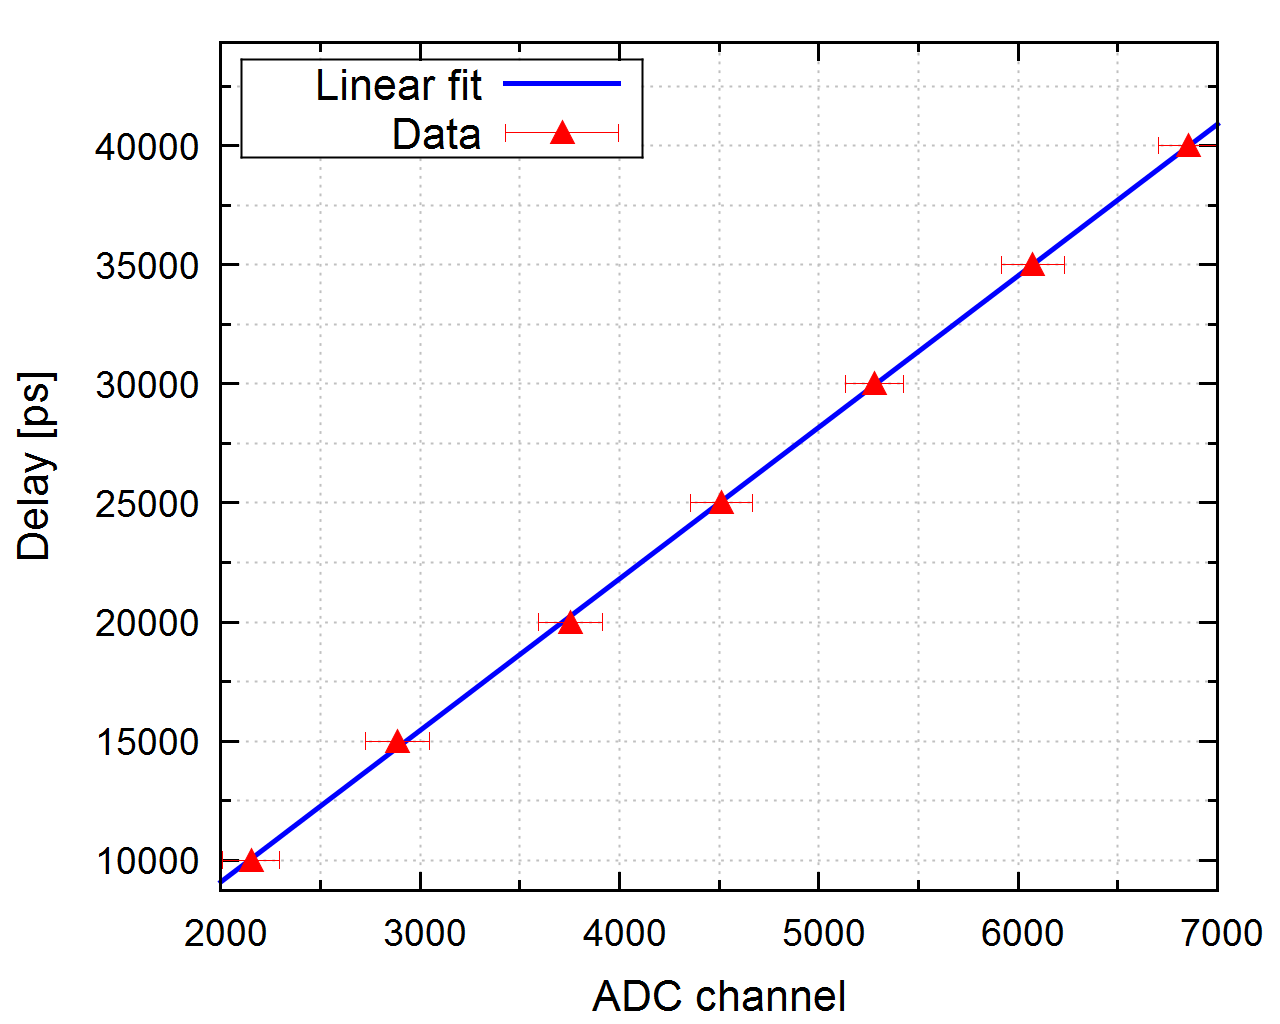
\includegraphics[width=0.49\textwidth]{./plots/timing/ze.png}}
	\hfill
	\caption[Time calibration]{Time calibration for different delays.}
	\label{fig:ch5:calibration}
\end{figure}
Since the net delay between signal one and two is random due to electronics and processing, a time calibration had to be made. For this, the \sr{} source was placed in the very middle of the scintillator (equally to the section before), so the time difference between coincident signals in detector one and two should be zero. By testing different delays with an adjustable delay box, the delay was set in a way that the peak of the resulting time spectrum was near the center of the acceptance of the ADC ($\approx$ channel 4000). By slightly increasing and decreasing the delay, the peak changes its position around the center. This yields a linear correlation between channel number $K$ and time $T$:
\begin{align*}
T(K)=\text{slope}\cdot K + T_0 = 6.3611\frac{\si{\nano\second}}{\text{ch}}\cdot K-23631\si{\nano\second}.
\end{align*}
The calibration spectrum and the linear fit are shown in figure \ref{fig:ch5:calibration}. The data for the linear fit was extracted by fitting Gaussians within the \texttt{root} framework to the peaks in the time spectrum. The error of each data point is given by the standard deviation of the Gaussian fit.\par      
Analog to the previous section, the \sr{} source was moved to different positions for determining the time resolution by measuring the standard deviation of the peak, and the propagation time by determining the position of the peak relative to the center. The threshold for both detectors was set to $\SI{-50}{\milli\volt}$, to detect the first incoming photons of each event for fastest response. 
This is visualized in figure \ref{fig:ch5:timing}. \par 
\begin{figure}[t!]
	\centering
	\subfloat[Measurement positions] {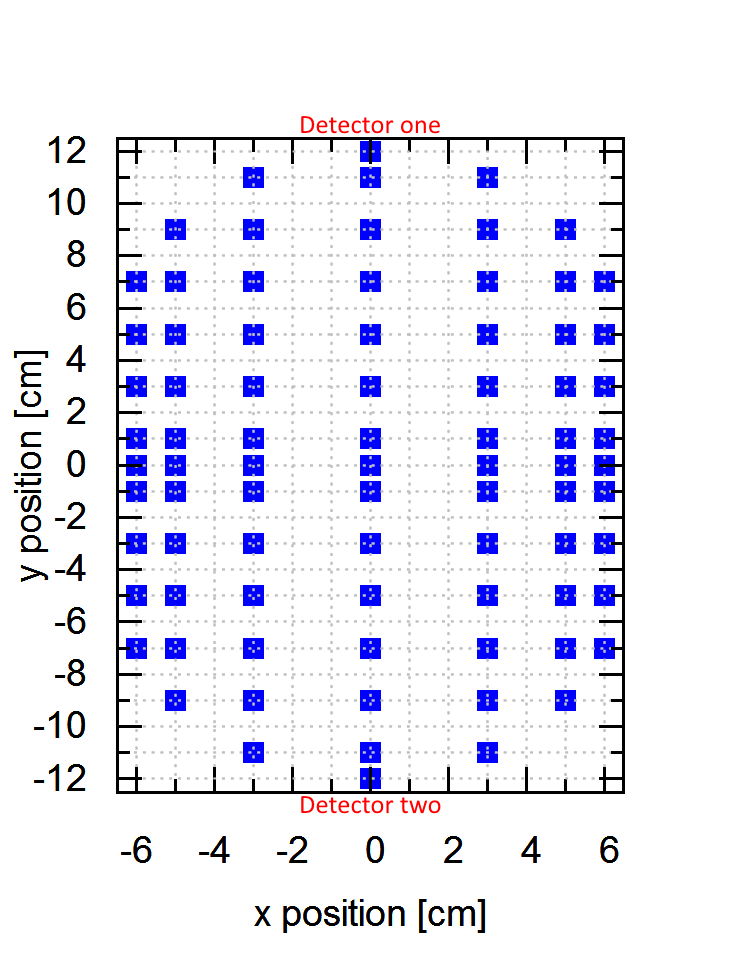
\includegraphics[width=0.33\textwidth]{./plots/timing/punkte.png}}
	\hfill
	\subfloat[Time resolution] {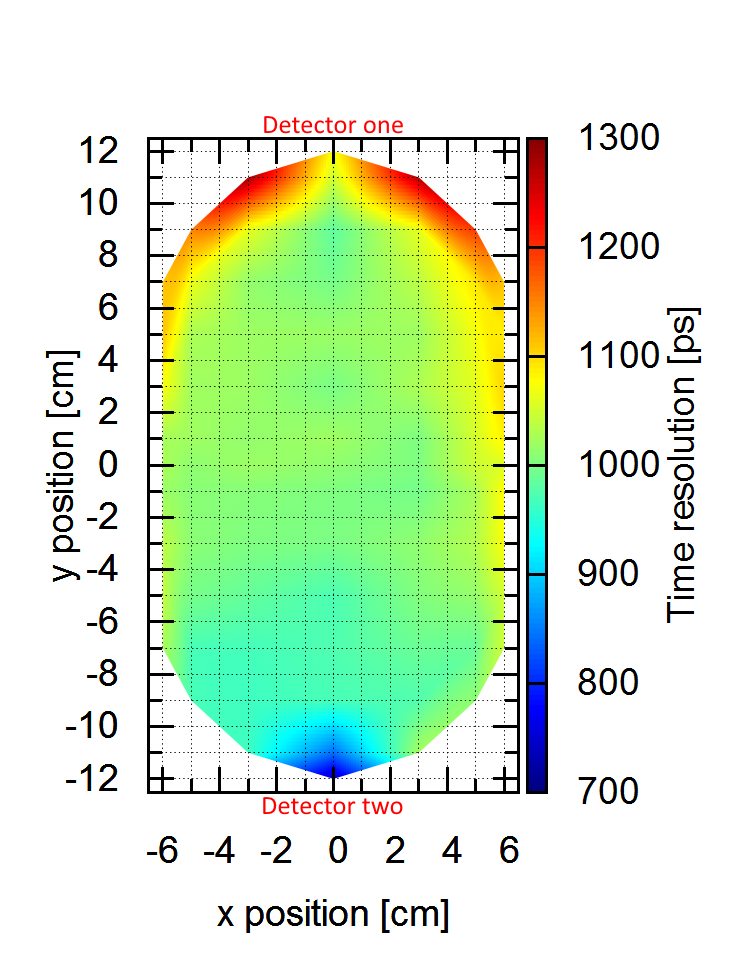
\includegraphics[width=0.33\textwidth]{./plots/timing/aufl.png}}
	\hfill
	\subfloat[Propagation time] {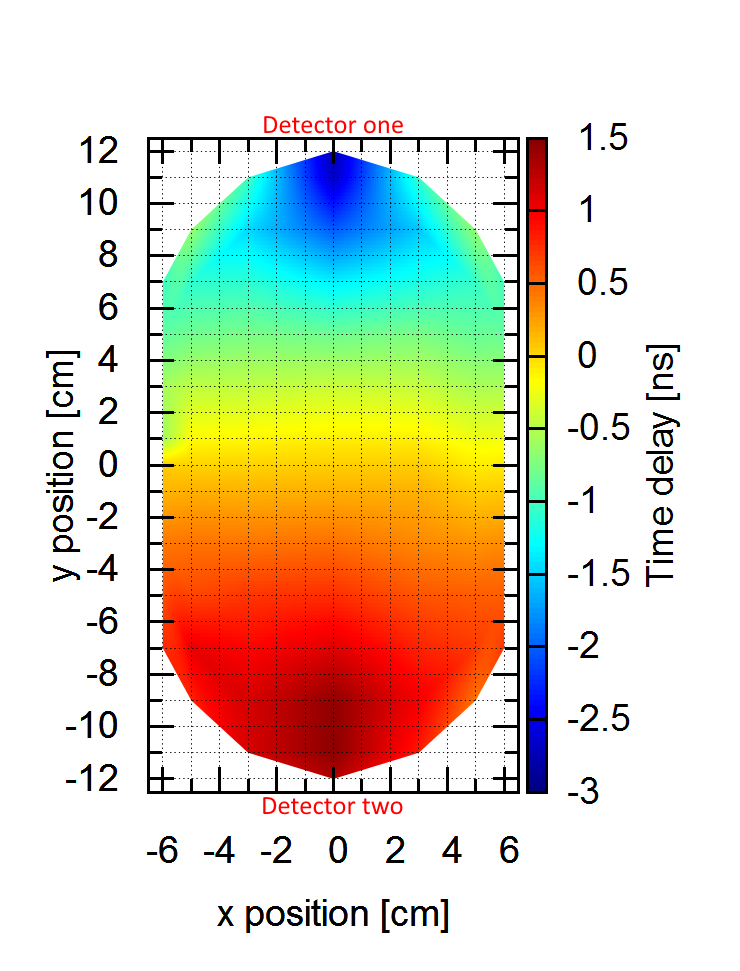
\includegraphics[width=0.33\textwidth]{./plots/timing/tof.png}}
	\hfill
	\caption[Timing reolution measurement]{Time resolution measurement at plastic scintillator with a \sr{} source at different positions. The heat map was plotted with \tit{gnuplot's pm3d} feature, the data between the data points was interpolated by the same software.}
	\label{fig:ch5:timing}
\end{figure}
Again, an obvious asymmetry can be observed. The time resolution right in front of detector two is best with approximately $\SI{700}{\pico\second}$ and rises to $\SI{1}{\nano\second}$ in the center of the scintillator. The resolution stays nearly stable but deteriorates towards the edges near detector one. \par 
This behavior is more pronounced when investigating the propagation time of the scintillation light. The theoretical propagation time for photons in medium is given by 
\begin{align}
T=\frac{s}{n^{-1}\cdot c_0},
\end{align}
where $s$ is the length, $n$ the refractive index ($n=1.58$ EJ-248M \cite{eljen}) for the medium and $c_0$ the speed of light in vacuum. Therefore, one expects
\begin{align*}
T_{\text{max}}=\frac{\SI{0.25}{\meter}}{1.58^{-1}\cdot\SI{299792458}{\meter\per\second}}\approx\SI{1300}{\pico\second}
\end{align*}
as the maximum propagation time, when the source is placed right in front of one detector. This can be found for detector two. Still, detector one shows nearly three times the expected result. \par 
\begin{figure}[t!]
	\centering
	\subfloat[The left peak represents the y position over detector one, right peak over detector two. The time distance between two peaks should represent the maximum propagation time of the photons.] {\includegraphics[width=0.49\textwidth]{./plots/timing/abst_hist.png}}
	\hfill
	\subfloat[Difference of relative timing between the detectors for the two extreme positions of the source] {\includegraphics[width=0.49\textwidth]{./plots/timing/abst.png}}
	\hfill
	\caption[Threshold dependence of the propagation time measurement]{Threshold dependence of the propagation time measurement.}
	\label{fig:ch5:threshold_dependenecy}
\end{figure}
To study this asymmetry, the threshold of both detectors was increased. A higher threshold suppresses the first photons arriving at the detector since they produce only a small signal. To overcome this, more photons are needed, so a signal is only generated when reflected photons are adding up to the signal as well, leading to a longer propagation time. Hence, for higher thresholds more delay can be expected. To show this behavior, the source was placed above detector one and then above detector two. The resulting time should be the travel time of photons for $2\times\SI{25}{\centi\meter}$ in the scintillator material and is represented by the horizontal distance of the two peaks plotted in figure \ref*{fig:ch5:threshold_dependenecy}. For $\SI{-50}{\milli\volt}$, the right peak (represents detector two) is ca. $\SI{1.5}{\nano\second}$ off center and satisfies the calculations. This can also be seen in figure \ref{fig:ch5:timing}b. The left peak, representing detector one, shows nearly $\SI{2.5}{\nano\second}$ delay. The peak of detector two moves to higher delays, which is expected due to reflections, whereas the peak for detector one stays at the same position until a threshold of $\SI{-300}{\milli\volt}$. For this and higher thresholds the peaks are distributed symmetrically to the y-axis. Still, this symmetry should occur for all thresholds. \par
An explanation for the asymmetry in the efficiency, time resolution and propagation time measurements might be dissimilar sensitivities of the two detectors. A good resolution is achieved when both detectors are exposed to a high amount of direct light, so seeing less direct light results in bad timing. One can assume, and the efficiency measurements confirms this, that, when the source is placed right in front of one detector, this detector sees sufficient direct light. Hence, bad timing in front of one detector is due to bad performance of the opposite detector. Therefore, detector one seems to perform better than its counterpart. \par 
\begin{figure}[t!]
	\centering
	\includegraphics[width=1\linewidth]{./graphics/ch5/scheme_energy.png}
	\caption[Schematic of the energy measurements]{Schematic of the energy measurements}
	\label{fig:ch5:scheme_energy}
\end{figure}
This problem might be overcome by fine tuning the thresholds and gains (biasing) of the detectors. To refer to figure \ref{fig:ch5:threshold_dependenecy}, the left peak represents the allegedly good working detector one. By rising the threshold, the peak remains at the same position until a certain level is exceeded. This might be an indicator that at this very point the reflected light dominates. This cannot be seen for detector two: a saturation where the peak is stable for distinct thresholds was not found. \par 
Further work on tuning the setup parameters as well as using up to date processing electronics might lead to a distinct increase in precision. 

\section{Energy measurements}

\begin{figure}[t!]
	\centering
	\subfloat[LYSO crystal, sized $\SI{10}{\milli\meter}\times\SI{10}{\milli\meter}\times\SI{3.5}{\milli\meter}$] {\includegraphics[width=0.49\textwidth]{./pictures/Crystal/lyso.jpg}}
	\hfill
	\subfloat[\pwo{} crystal (sized $\SI{20}{\milli\meter}\times\SI{20}{\milli\meter}\times\SI{50}{\milli\meter}$) with the $3\times 2$ matrix-board] {\includegraphics[width=0.49\textwidth]{./pictures/Crystal/lyso_board.jpg}}
	\hfill
	\caption[LYSO and \pwo{} crystals]{LYSO and \pwo{} crystals with the $3\times 2$ matrix SiPM-board.}
	\label{fig:ch5:crystals}
\end{figure}

Another application for SiPMs could be the usage in calorimetry, measuring deposited energy of particles in scintillators. Some prominent inorganic scintillator crystals were used, LYSO ($\SI{10}{\milli\meter}\times\SI{10}{\milli\meter}\times\SI{3.5}{\milli\meter}$) and \pwo{} ($\SI{20}{\milli\meter}\times\SI{20}{\milli\meter}\times\SI{50}{\milli\meter}$), to measure several $\gamma$-spectra from calibration sources. \par 
The small LYSO crystal was equipped with a $2\times 1$ parallel SiPM-configuration. The board was attached with optical grease to the $\SI{10}{\milli\meter}\times\SI{10}{\milli\meter}$ surface, the other sides of the crystal were covered with reflective tape. For stability and lightproofing, this combination was then wrapped in black tape. \par 
The \pwo{} crystal was wrapped in eight layers of Teflon foil, one thin layer of aluminum foil and fixed with shrinking tube, leaving the front surface ($\SI{20}{\milli\meter}\times\SI{20}{\milli\meter}$) uncovered. On this side, a $3\times 2$ parallel SiPM-configuration was attached analogous to previous setups, see figure \ref{fig:ch5:crystals}. \par
Using a \textit{KETEK} preamplifier \cite{ketek_preamp}, the crystals were set up in the climate chamber (\tit{WEISS}, see figure \ref{fig:ch5:scheme_energy}). The amplified signal was further shaped by a linear amplifier (Ortec 410) with adjustable integration time and gain. The energy spectrum was taken by an analog-to-digital converter from Caen (N957) which was controlled by a UNIX-workstation. \par   

\subsection{LYSO}
First, the LYSO crystal was tested at $\SI{-25}{\degreeCelsius}$ under $\gamma$-radiation from a \co{} source. It appeared that the raw signal of the two SiPMs in parallel was so strong that the preamplifier saturated, so the bias voltage was set to $\SI{26}{\volt}$ right beyond breakdown. The same problem with the linear amplifier was solved by using a $\SI{-20}{\decibel}$ passive attenuator. By choosing $\SI{2}{\micro\second}$ integration time and a proper amplification, the gain was set in a way that the photopeaks of \co{} were between channel 5000 and 6000 to use the full range of the $13$-bit analog-to-digital converter.  \par  
Consecutively, the energy spectra of several calibration sources (\co{}, \na{}, \cs{}, \ba{} and \eu{}) were taken. To calibrate the setup, the most prominent photopeaks were fitted with Gaussians. The calibration fit is depicted in figure \ref{fig:ch5:lyso_eichung}, the spectra are plotted in figure \ref{fig:ch5:lyso_energy}. The same procedure was done at $\SI{25}{\degreeCelsius}$, where the amplification of the linear amplifier had to be increased by a factor of 4. \par 
The photopeak of \ba{} is distinct as well as the x-ray peak at low energies. The cobalt spectrum has a large compton background since the gamma quanta with $\SI{1.1}{\MeV}$ and $\SI{1.3}{\MeV}$ (all gamma ray energy data is retrieved from \cite{gamma_energy}) are too energetic to be fully stopped in the $\SI{3.5}{\milli\meter}$ thick crystal. For this, the two photopeaks are barely visible, the sum peak could not be observed at all. Furthermore, \cs{} and \na{} show a clear photopeak and a distinct compton spectrum, the $\SI{511}{\keV}$ peak due to annihilation of the positron from the $\beta^+$ decay of sodium is clearly visible. The \eu{} source was tested as a calibration source since the spectrum shows multiple gamma energies and it was found that the most prominent peaks ($\SI{344}{\keV}$, $\SI{244}{\keV}$, $\SI{121}{\keV}$, $\SI{40}{\keV}$) could be resolved, especially for $\SI{-25}{\degreeCelsius}$. More detailed energy spectra plots can be found in \ref{ap:energy_spectra}.  \par 
The energy resolution $R$, defined as the ratio of \tit{full width at half maximum} (FWHM) and photoenergy, was calculated as well. The whole data is given in \ref{ap:B:tab:energy_spectra}. The resolution is plotted in figure \ref{fig:ch5:lyso_resolution}. The resolution of the cooled system is in some cases ($\SI{300}{\keV}$ to $\SI{700}{\keV}$) slightly better. For low and high energies, larger errors can be found. 
\par 
\begin{figure}[t!]
	\floatbox[{\capbeside\thisfloatsetup{capbesideposition={left,center},capbesidewidth=0.45\linewidth}}]{figure}[\FBwidth]
	{\caption[Energy resolution for the LYSO crystal setup]{Energy resolution for the LYSO crystal setup. The photo peaks for $\SI{244.7}{\keV}$ and $\SI{1173.2}{\keV}$ were not distinct at $\SI{25}{\degreeCelsius}$ and therefore were not fitted. Hence, some of the error bars are large. }    
		\label{fig:ch5:lyso_resolution}}
	{\includegraphics[width=0.55\textwidth]{./plots/energy/lyso_resolution.png}}
\end{figure} 
Cooling does not seem to improve the energy reolution significantly, despite the intrinsic dark noise of the SiPM is suppressed and the light yield of the scintillator is improved. The strong raw signal indicates that a lot of scintillation light is seen by the SiPMs. 
\begin{figure}[H]
	\centering
	\includegraphics[width=1\linewidth]{./plots/energy/lyso_eichung.png}
	\caption[LYSO energy calibration]{Energy calibration with different sources using the LYSO crystal.}
	\label{fig:ch5:lyso_eichung}
\end{figure} 
\begin{figure}[H]
	\centering
	\includegraphics[width=1\linewidth]{./plots/energy/lyso_energy.png}
	\caption[LYSO energy spectra]{Energy spectra of several calibration sources using the LYSO crystal.}
	\label{fig:ch5:lyso_energy}
\end{figure}
\newpage
\noindent
According to table \ref{ch2:tab:characteristics}, LYSO is a very bright scintillator with 30000 photons per $\SI{511}{\keV}$ photon, even higher when cooled. The SiPMs seem to be overexerted due to this large amount of photons. This might be solved by a higher number of microcells (smaller pixel size), so more photons can be detected at the same time. This overextension could be the reason why cooling does not result in a significant better resolution. Still, an improvement by cooling is expected for crystals with lower light yield, i.e. lead tungstate, which will be covered in next section.      

\subsection{\pwo{}}

The lead tungstate setup with six parallel SiPMs is operated comparable to the LYSO setup with two SiPMs. However, the light yield of \pwo{} is several orders of magnitude lower (\ref{ch2:tab:characteristics}) than LYSO, and roughly $85-110$ photons per $\si{\MeV}$ are expected \cite{panda_emctdr}.\par 
\begin{figure}[b!]
	\centering
	\includegraphics[width=1\linewidth]{./plots/energy/pwo_energy.png}
	\caption[\pwo{} energy spectra]{\pwo{} energy spectra of several calibration sources.}
	\label{fig:ch5:pwo_energy}
\end{figure}
Figure \ref{fig:ch5:pwo_energy} shows the energy spectra of several calibration sources. At higher temperature ($\SI{25}{\degreeCelsius}$), the energy spectra merge with the background. At this point, one has to consider the \tit{photo detection efficiency} (PDE) of the SiPMs ($\approx 40\%$) for the emission wavelength of \pwo{} ($\SI{425}{\nano\meter}$), the loss of photons due to absorption ($\approx 10\%$) and the effective light sensitive area (ratio of the sensitive area of the SiPM and the $\SI{20}{\milli\meter}\times\SI{20}{\milli\meter}$ crystal surface, about $13.5$\%). Hence, only few photons are left, diminishing the resolution of the spectrum. The measurements at $\SI{25}{\degreeCelsius}$ show that only for a small amount of events a sufficient number of photons are registered to fill bins beyond the background. However, this is not sufficient for determining the particle energy. \par 
The spectra at $\SI{-25}{\degreeCelsius}$ are more distinct: \co{} shows a broad and flat peak in which the two photopeaks are merged. The \na{} spectrum shows both the annihilation peak and the photopeak at $\SI{1275}{\keV}$, so does the \cs{} spectrum at $\SI{662}{\keV}$. The background shows less noise compared to the background at $\SI{25}{\degreeCelsius}$. Reason being the higher light yield ($\approx \times 3.5$ \cite{panda_emctdr}) and the suppressed thermal noise of the SiPMs. A small peak at channel 5000 is also visible and will be discussed in the following section. \par 
\subsection{Muons}
The \pwo{} setup was also used to measure the energy deposit of cosmic muons in lead tungstate. According to \cite{panda_emctdr}, the energy deposit for minimum ionizing particles is $\SI{10.2}{\MeV\per\centi\meter}$, so one expects a mean energy loss of $\approx \SI{20}{\MeV}$ in the crystal with a thickness of $\SI{2}{\centi\meter}$. Since the energy deposit of cosmic muons in matter varies due to the statistical nature of the energy loss, whose mean value is given by the Bethe-Bloch-formula (see equation \eqref{eq:bethe_bloch}), a Landau distribution with a peak at $\approx \SI{20}{\MeV}$ is expected. \par 
Since the light yield is higher and the noise is suppressed at low temperatures, the \pwo{} was cooled down to $\SI{-25}{\degreeCelsius}$. A \co{} spectrum was taken to calibrate the range of the analog-to-digital converter, the spectrum can be seen in figure \ref{fig:ch5:muon_spectrum}. The gain was adjusted to set the energy range of the ADC from $\SI{0}{\MeV}$ to $\SI{40}{MeV}$. After removing the calibration source, data was taken for $\SI{48}{\hour}$ due to the small flux of muons through the crystal. The resulting spectrum is shown in the same figure.  \par 
A large background can be found in the first 2000 channels. By comparison with the calibration spectrum of \co{}, it appears that several other gamma sources, either intrinsic or natural environmental radiation, with energies up to $\SI{2}{\MeV}$ contribute to the muon spectrum. A possible candidate is \ka{} with a gamma energy of $\SI{1460.9}{\keV}$, which not only is present in the environment but also as part of the crystal (impurity, up to $0.48$ ppm \cite{analytical_report}). The muon spectrum itself is broad and flat and shows no Landau distribution at all. This might be caused by the geometry of the setup when muons travel through more or less than $\SI{2}{\centi\meter}$ of crystal and hence lose not exactly $\SI{20}{\MeV}$ of energy. This could cause the spectrum to show no distinct Landau peak. \par 
\begin{figure}[b!]
	\centering
	\subfloat[Energy spectrum without any trigger and small range] {\includegraphics[width=0.49\textwidth]{./plots/energy/Muons_ohne_Trigger.png}}
	\hfill
	\subfloat[Energy spectrum with upper and lower trigger and wide range] {\includegraphics[width=0.49\textwidth]{./plots/energy/muon_both_trigger.png}}
	\hfill
	\caption[Energy loss spectrum of cosmic muons]{Energy loss spectrum of cosmic muons. Picture (a) shows a large intrinsic background.}
	\label{fig:ch5:muon_spectrum}
\end{figure}
As a solution for this problem, a trigger system  consisting of two plastic scintillator bars with photomultiplier tube readout was utilized. Using one bar as an upper and one bar as a lower trigger, the two plastics were placed above and under the \pwo{} crystal. The coincident trigger signal gates the ADC, therefore only events measured in all three scintillators were added to the spectrum. The data is plotted in figure \ref{fig:ch5:muon_spectrum}. \par 
The first set of data, plot (a), was taken with a smaller energy range and without trigger system. The calibration spectrum was set to roughly $\SI{1200}{\keV}$ at channel 400, using the double peak of \co{}. The trigger system was then introduced since no peak could be observed and due to the large background. Plot (b) shows that the energy range is larger than before whereas the calibration peak could not be used as intended because of the nonlinearity of the ADC in small channel values. A peak at channel 4000 can be observed and the Landau distribution can be guessed. At lower channels (200 to 3000), smaller energy values due to geometrical effects are visible, for the plastic scintillator bars are larger as the \pwo{} crystal and therefore transition paths smaller than $\SI{2}{\centi\meter}$ are possible for muons.  






  





\chapter{Summary and outlook}

The development and characterization of the SiPM-based readout-board was a major part of this thesis. Measuring the temperature dependency of the breakdown and operation voltage brought insight into the diverse behavior of the different boards.\par 
The single SiPM showed the expected behavior with exponentially increasing current beyond breakdown, whereas the parallel and hybrid configurations had even higher currents. The data provided by \tit{KETEK} for the temperature coefficient $k_{BD}$ of the SiPMs used were confirmed for all configurations and the coefficient $k_{OP}$ of the operation voltage was found to be slightly different between the single and hybrid/parallel configurations. This might be due to  differences in production conditions between the individual SiPMs and may be solved by characterizing each SiPM by means of the temperature coefficients and IV-characteristics. Matching similar diodes enables one to adjust breakdown and operation voltage precisely. \par 
This behavior was also found by taking the dark spectra. The unique discrete spectrum could only be found for a single SiPM, whereas multiple diodes only showed a blurred picture. By matching similar SiPMs, this could be improved, since knowledge about the thermal noise enables one to set the threshold right above a certain number of cells firing to get a good signal-to-noise ratio. The count rate for multiple SiPMs was found to be roughly $N$ times as high as the rate of a single SiPM, where $N$ is the number of diodes used. For a single SiPM, the slope of the count rate again showed the stepwise behavior, although multiple SiPMs did not. The slope for the hybrid configuration was found to be twice ($\sqrt{N}=2$) as high as the rate for a single or parallel SiPMs. \par 
By comparing the raw signals of the different configurations attached to the plastic scintillator \tit{EJ-248M}, it was discovered that the height of the single and parallel configurations are equal and twice as high as for the hybrid configuration. Again, there is a $\sqrt{N}$ dependence as proposed by \cite{sebastian}. Using the preamplifier showed that the hybrid configuration in fact has the shortest rise time compared with a single diode and the parallel configuration, which has the longest one. \par 
When it came to mechanically mounting the boards, one benefits by the chosen design of the board: due to its small size it was easily attached to the thin sides of the scintillator plate and was supported by the design of the spacing masks with reflective foil. Coupling to the crystals was simpler as anticipated because of various possibilities of arranging the SiPMs on the board and even daisy-chaining two or more boards electrically. \par 
One downside of this design is the connection between board and preamplifier: using a coaxial cable led to a huge amount of noise and ringing. This was avoided by directly connecting the boards via pin headers, which made the whole setup unhandy. Prospective versions of the SiPM-board are planned to integrate an on-board preamplifier. \par 
The efficiency measurements delivered an ambivalent result: even though the plastic scintillator plate and the SiPM-setup was designed symmetrically, an asymmetric result was yielded. Despite the count rate of both boards showed similar behavior, one detector was nearly twice as efficient in counting at certain positions, i.e. in front of its opposite detector. This circumstance was again observed in the timing resolution and propagation time measurement. The resolution ranged from $\SI{700}{\pico\second}$ up to $\SI{1300}{\pico\second}$. The results of the propagation time measurement suggests that the less effective detector should have been adjusted more carefully in terms of threshold and gain. Nevertheless, one of two detectors showed sufficient performance and by using more up-to-date processing electronics an even better time resolution might have been achieved. \par 
The energy measurement with the small LYSO crystal yielded some interesting energy spectra of the calibration sources and reached resolutions ranging from $20\%$ to $30\%$ depending on the source. Since cooling did not improve the energy resolution significantly, the conclusion has been drawn that the number and the size of the microcells might be a crucial factor. Shrinking the size and increasing the number of microcells should improve the sensitivity of the SiPM coupled to a bright scintillator. KETEK claims \cite{ketek_preamp} that a new series of SiPMs with a microcell size of $\SI{15}{\micro\meter}$ reaches a resolution of $13\%$ for the $\SI{511}{\keV}$ peak at a comparably small LYSO crystal. \par 
The daisy-chaining of two SiPM-boards created a $3\times 2$ matrix of parallel SiPMs to be attached to a small volume \pwo{} crystal. At room temperature, the energy spectra of the sources were barely distinguishable from the background and noise of the setup. When cooled, due to higher light yield and lower noise, several spectra could be taken and one was able to identify the photopeaks, yet the resolution was poor, as expected. For lightweak scintillators, SiPMs with larger microcells might be more suitable to choose since only few photons have to be detected and noise will be smaller. \par 
The muon measurements demonstrated that the \pwo{} shows a significant intrinsic background which was avoided by using a trigger system consisting of two plastic scintillators with photomultiplier tube readout. These precautions yielded a distinct energy loss spectrum of cosmic muons. 










 



	
\clearpage
\newpage



\begin{appendices}
	
% !TEX root = Nies_Lukas_BSc_Thesis_SiPM.tex

%Use letters for appendix referencing
%\renewcommand\thefigure{\thesection.\arabic{figure}} 

\chapter{Figures}

%\setcounter{figure}{0}    

\begin{figure}[H]
	\centering
	\includegraphics[width=0.65\textwidth]{./graphics/ch1/photo_absorption_cross_sections.png}
	\caption[Interaction of phtonos with matter (detailed)]{Energy dependence of the cross-section of photons in carbon and lead \cite{wermes}.}    
	\label{ap:A:photons_detailed}
\end{figure}

\newpage

\begin{figure}[t]
	\centering
	\includegraphics[width=0.85\textwidth]{./graphics/ch1/bethe_bloch_detailed.png}
	\caption[Stopping power for a wide energy range]{Stopping power for a wide energy range \cite{PDG}. The \textit{Bethe-Bloch} region is shown for $0.1<\beta\gamma<1000$.}    
	\label{ap:A:bethe_bloch_detailed}
\end{figure}

\newpage

\begin{figure}[t]
	\centering
	\includegraphics[width=0.85\textwidth]{./graphics/ch2/jablonski.png}
	\caption[Jablonski-Diagram]{Jablonski-Diagram for singlet and triplet states of $\pi$-electrons of a organic scintillator \cite{wermes}.}    
	\label{ap:A:jablonski}
\end{figure}

\chapter{Fits, Plots and data processing}

\section{IV-curves}

First, the region before breakdown has been fitted with a first order polynomial 
\begin{align*}
I(V)=m\cdot V+I_0
\end{align*} 
to find the offset $I_0$. This has then been substracted from the data to grant more precision when plotting $I$ in log scale. Now two polynomial functions have been used to determine the intersection of the point of breakdown
\begin{align*}
\log(I(V))&=m\cdot V+I_{0} & \log(I(V))&=A\cdot V^2+B\cdot V+C.
\end{align*}
By comparing both equations and solving V, one retrieves 
\begin{align*}
m\cdot V+I_{0} &= A\cdot V^2+B\cdot V+C \\
\Rightarrow V_{\pm} &= -\frac{B-m}{2A}\pm \sqrt{\left(\frac{B-m}{2A}\right)^2-\frac{C-I_0}{A}}, 
\end{align*}
where $V_\pm$ is the solution of this equation. The error $\Delta V$ has been calculated via error propagation of the fit errors:
\begin{align*}
\Delta V_\pm=\arrowvert\dv{V_\pm}{m}\arrowvert\Delta m+\arrowvert\dv{V_\pm}{I_0}\arrowvert\Delta I_0+\arrowvert\dv{V_\pm}{A}\arrowvert\Delta A+\arrowvert\dv{V_\pm}{B}\arrowvert\Delta B+\arrowvert\dv{V_\pm}{C}\arrowvert\Delta 
C.
\end{align*}
The fits can be found in figures \ref{ap:B:breakdown_fits_single} and \ref{ap:B:breakdown_fits_hybrid}.

\newpage

\begin{figure}[H]
	\subfloat[(s)-configuration $\SI{25}{\degreeCelsius}$] {\includegraphics[width=0.49\textwidth]{./plots/iu_curve/1x1n2_bd_25.png}}
	\hfill
	\subfloat[(s)-configuration $\SI{20}{\degreeCelsius}$] {\includegraphics[width=0.49\textwidth]{./plots/iu_curve/1x1n2_bd_20.png}}
	\hfill
	\subfloat[(s)-configuration $\SI{15}{\degreeCelsius}$] {\includegraphics[width=0.49\textwidth]{./plots/iu_curve/1x1n2_bd_15.png}}
	\hfill
	\subfloat[(s)-configuration $\SI{10}{\degreeCelsius}$] {\includegraphics[width=0.49\textwidth]{./plots/iu_curve/1x1n2_bd_10.png}}
	\hfill
	\subfloat[(s)-configuration $\SI{5}{\degreeCelsius}$] {\includegraphics[width=0.49\textwidth]{./plots/iu_curve/1x1n2_bd_5.png}}
	\hfill
	\subfloat[(s)-configuration $\SI{0}{\degreeCelsius}$] {\includegraphics[width=0.49\textwidth]{./plots/iu_curve/1x1n2_bd_0.png}}
	\hfill
	\subfloat[(s)-configuration $\SI{-25}{\degreeCelsius}$] {\includegraphics[width=0.38\textwidth]{./plots/iu_curve/1x1n2_bd_-25.png}}
	\hfill
	\caption[Breakdown fits (single)]{Fits for determining the breakdown of a single SiPM. }
	\label{ap:B:breakdown_fits_single}
\end{figure}

\newpage

\begin{figure}[H]
	\subfloat[(h)-configuration $\SI{25}{\degreeCelsius}$] {\includegraphics[width=0.49\textwidth]{./plots/iu_curve/4x1n6_bd_25.png}}
	\hfill
	\subfloat[(h)-configuration $\SI{20}{\degreeCelsius}$] {\includegraphics[width=0.49\textwidth]{./plots/iu_curve/4x1n6_bd_20.png}}
	\hfill
	\subfloat[(h)-configuration $\SI{15}{\degreeCelsius}$] {\includegraphics[width=0.49\textwidth]{./plots/iu_curve/4x1n6_bd_15.png}}
	\hfill
	\subfloat[(h)-configuration $\SI{10}{\degreeCelsius}$] {\includegraphics[width=0.49\textwidth]{./plots/iu_curve/4x1n6_bd_10.png}}
	\hfill
	\subfloat[(h)-configuration $\SI{5}{\degreeCelsius}$] {\includegraphics[width=0.49\textwidth]{./plots/iu_curve/4x1n6_bd_5.png}}
	\hfill
	\subfloat[(h)-configuration $\SI{0}{\degreeCelsius}$] {\includegraphics[width=0.49\textwidth]{./plots/iu_curve/4x1n6_bd_0.png}}
	\hfill
	\subfloat[(h)-configuration $\SI{-25}{\degreeCelsius}$] {\includegraphics[width=0.38\textwidth]{./plots/iu_curve/4x1n6_bd_-25.png}}
	\hfill
	\caption[Breakdown fits (hybrid)]{Fits for determining the breakdown of a hybrid board. }
	\label{ap:B:breakdown_fits_hybrid}
\end{figure}

\newpage

\section{Operation voltage}

The relative slope $\dv{I}{V}\frac{1}{I(V)}$ shows a minimum some volts beyond breakdown. A second order polynomial function was used for determining the minimum:
\begin{align*}
I(V)&=A\cdot V^2+B\cdot V+C.
\end{align*}
The minimum can be found by deriving and zeroing:
\begin{align*}
\dv{I(V)}{V}&\overset{!}{=}0 \\
\Rightarrow V_0&=-\frac{B}{2A}.
\end{align*}
The error is again calculated by error propagation 
\begin{align*}
\Delta V_0=\arrowvert\dv{V_0}{A}\arrowvert\Delta A+\arrowvert\dv{V_0}{B}\arrowvert\Delta B.
\end{align*}
The fits can be found in figures \ref{ap:B:optimal_fits_single} and \ref{ap:B:optimal_fits_hybrid}.

\newpage

\begin{figure}[H]
	\subfloat[(s)-configuration $\SI{25}{\degreeCelsius}$] {\includegraphics[width=0.49\textwidth]{./plots/iu_curve/1x1n2_op_25.png}}
	\hfill
	\subfloat[(s)-configuration $\SI{20}{\degreeCelsius}$] {\includegraphics[width=0.49\textwidth]{./plots/iu_curve/1x1n2_op_20.png}}
	\hfill
	\subfloat[(s)-configuration $\SI{15}{\degreeCelsius}$] {\includegraphics[width=0.49\textwidth]{./plots/iu_curve/1x1n2_op_15.png}}
	\hfill
	\subfloat[(s)-configuration $\SI{10}{\degreeCelsius}$] {\includegraphics[width=0.49\textwidth]{./plots/iu_curve/1x1n2_op_10.png}}
	\hfill
	\subfloat[(s)-configuration $\SI{5}{\degreeCelsius}$] {\includegraphics[width=0.49\textwidth]{./plots/iu_curve/1x1n2_op_5.png}}
	\hfill
	\subfloat[(s)-configuration $\SI{0}{\degreeCelsius}$] {\includegraphics[width=0.49\textwidth]{./plots/iu_curve/1x1n2_op_0.png}}
	\hfill
	\subfloat[(s)-configuration $\SI{-25}{\degreeCelsius}$] {\includegraphics[width=0.38\textwidth]{./plots/iu_curve/1x1n2_op_-25.png}}
	\hfill
	\caption[Operation voltage fits (single)]{Fits for determining the operation voltage of a single SiPM. }
	\label{ap:B:optimal_fits_single}
\end{figure}

\newpage

\begin{figure}[H]
	\subfloat[(s)-configuration $\SI{25}{\degreeCelsius}$] {\includegraphics[width=0.49\textwidth]{./plots/iu_curve/4x1n6_op_25.png}}
	\hfill
	\subfloat[(s)-configuration $\SI{20}{\degreeCelsius}$] {\includegraphics[width=0.49\textwidth]{./plots/iu_curve/4x1n6_op_20.png}}
	\hfill
	\subfloat[(s)-configuration $\SI{15}{\degreeCelsius}$] {\includegraphics[width=0.49\textwidth]{./plots/iu_curve/4x1n6_op_15.png}}
	\hfill
	\subfloat[(s)-configuration $\SI{10}{\degreeCelsius}$] {\includegraphics[width=0.49\textwidth]{./plots/iu_curve/4x1n6_op_10.png}}
	\hfill
	\subfloat[(s)-configuration $\SI{5}{\degreeCelsius}$] {\includegraphics[width=0.49\textwidth]{./plots/iu_curve/4x1n6_op_5.png}}
	\hfill
	\subfloat[(s)-configuration $\SI{0}{\degreeCelsius}$] {\includegraphics[width=0.49\textwidth]{./plots/iu_curve/4x1n6_op_0.png}}
	\hfill
	\subfloat[(s)-configuration $\SI{-25}{\degreeCelsius}$] {\includegraphics[width=0.38\textwidth]{./plots/iu_curve/4x1n6_op_-25.png}}
	\hfill
	\caption[Operation voltage fits (hyrbid)]{Fits for determining the operation voltage of a hybrid board. }
	\label{ap:B:optimal_fits_hybrid}
\end{figure}

\newpage

\section{Derivation methodology} \label{ap:B:sec:derivation}

For deriving a set of data consisting $x$ and $y$ values with $y(x)$, a linear regression algorithm has been implemented in \texttt{C++}. It fits a linear function 
\begin{align*}
y(x)=m\cdot x+y_0 
\end{align*}
to a number $n$ of data points where the data point lies right in the middle of the interval, so $\frac{n-1}{2}$ data points before and after will be included. This necessitates $n$ to be odd and $>3$.

\section{Energy spectra} \label{ap:energy_spectra}

The data of the fits for the energy spectra of the LYSO crystal is given in table \ref{ap:B:tab:energy_spectra}, more detailed plots can be seen in figure \ref{ap:B:energy_spectra1}. 

% Table generated by Excel2LaTeX from sheet 'Tabelle1'
\begin{table}[H]
	\small
	\centering
	\makebox[\textwidth]{
	\begin{tabular}{c|ccccc}
		\toprule[2pt]
		Source & Energy [$\si{\keV}$] & $\mu$ & $\sigma$ & FWHM [$\si{\keV}$] & $R$ [\%] \\
		\midrule
		& \multicolumn{5}{c}{$T=\SI{25}{\degreeCelsius}$} \\
		\eu{} & 121.80 & 321.92 $\pm$ 1.57  & 35.74 $\pm$ 7.56  & 22.62 $\pm$ 4.78  & 18.57 $\pm$ 3.93 \\
		\eu{} & 344.00 & 1238.11 $\pm$ 1.74  & 172.53 $\pm$ 17.16 & 109.20 $\pm$ 10.86 & 31.74 $\pm$ 3.16 \\
		\ba{} & 356.00 & 1260.24 $\pm$ 0.46  & 234.40 $\pm$ 1.38  & 148.35 $\pm$ 0.87  & 41.67 $\pm$ 0.25 \\
		\na{} ($e^+$) & 511.00 & 2085.84 $\pm$ 1.01 & 204.30 $\pm$ 3.53  & 129.30 $\pm$ 2.23  & 25.30 $\pm$ 0.44 \\
		\cs{} & 661.60 & 2373.58 $\pm$ 0.49  & 219.77 $\pm$ 2.64  & 139.09 $\pm$ 1.67  & 21.02 $\pm$ 0.25 \\
		\na{}  & 1274.50 & 4736.84 $\pm$ 6.01  & 399.79 $\pm$ 869.50 & 253.03 $\pm$ 550.32 & 19.85 $\pm$ 43.18 \\
		\co{} & 1252.90 & 4512.80 $\pm$ 5.67  & 516.36 $\pm$ 11.55 & 326.81 $\pm$ 7.31  & 26.08 $\pm$ 0.58 \\ 
		 & \multicolumn{5}{c}{$T=\SI{-25}{\degreeCelsius}$} \\
		\eu{} & 121.80 & 348.85 $\pm$ 0.46  & 55.21 $\pm$ 6.98  & 33.64 $\pm$ 4.25  & 27.62 $\pm$ 3.49 \\
		\eu{} & 244.70 & 883.46 $\pm$ 7.48  & 154.32 $\pm$ 794.50 & 94.03 $\pm$ 484.09 & 38.43 $\pm$ 197.83 \\
		\eu{} & 344.00 & 1379.17 $\pm$ 1.21  & 124.19 $\pm$ 6.15  & 75.67 $\pm$ 3.75  & 22.00 $\pm$ 1.09 \\
		\ba{} & 356.00 & 1230.25 $\pm$ 0.45  & 195.05 $\pm$ 1.18  & 118.84 $\pm$ 0.72  & 33.38 $\pm$ 0.20 \\
		\na{} ($e^+$) & 511.00 & 2111.80 $\pm$ 0.76 & 177.61 $\pm$ 1.93  & 108.22 $\pm$ 1.18  & 21.18 $\pm$ 0.23 \\
		\cs{} & 661.60 & 2189.56 $\pm$ 0.49  & 201.51 $\pm$ 4.79  & 122.78 $\pm$ 2.92  & 18.56 $\pm$ 0.44 \\
		60Co  & 1173.20 & 4132.47 $\pm$ 25.52 & 240.11 $\pm$ 92.17 & 146.30 $\pm$ 56.16 & 12.47 $\pm$ 4.79 \\
		\co{} & 1274.50 & 5011.38 $\pm$ 3.26  & 357.95 $\pm$ 8.16  & 218.10 $\pm$ 4.97  & 17.11 $\pm$ 0.39 \\
		\co{} & 1252.90 & 5111.35 $\pm$ 4.96  & 1096.87 $\pm$ 316.93 & 668.32 $\pm$ 193.10 & 53.34 $\pm$ 15.41 \\
		\bottomrule[2pt]
	\end{tabular}%
	}
	\caption{Fits for the energy spectra.}
	\label{ap:B:tab:energy_spectra}%
\end{table}%

\newpage

\begin{figure}[h]
	\subfloat[\eu{} energy calibration spectrum for $\SI{25}{\degreeCelsius}$] {\includegraphics[width=0.49\textwidth]{./plots/energy/lyso_eu25.png}}
	\hfill
	\subfloat[\eu{} energy calibration spectrum for $\SI{-25}{\degreeCelsius}$] {\includegraphics[width=0.49\textwidth]{./plots/energy/lyso_eu-25.png}}
	\hfill
	\subfloat[\ba{} energy calibration spectrum for $\SI{25}{\degreeCelsius}$] {\includegraphics[width=0.49\textwidth]{./plots/energy/lyso_ba25.png}}
	\hfill
	\subfloat[\ba{} energy calibration spectrum for $\SI{-25}{\degreeCelsius}$] {\includegraphics[width=0.49\textwidth]{./plots/energy/lyso_ba-25.png}}
	\hfill
	\subfloat[\co{} energy calibration spectrum for $\SI{25}{\degreeCelsius}$] {\includegraphics[width=0.49\textwidth]{./plots/energy/lyso_co25.png}}
	\hfill
	\subfloat[\co{} energy calibration spectrum for $\SI{-25}{\degreeCelsius}$] {\includegraphics[width=0.49\textwidth]{./plots/energy/lyso_co-25.png}}
	\hfill
	\caption[LYSO energy calibration spectra (detailed)]{Higher resolution energy calibration spectra. Continuation on next page. }
	\label{ap:B:energy_spectra1}
\end{figure}



\begin{figure}[h]
	\ContinuedFloat
	\subfloat[\cs{} energy calibration spectrum for $\SI{25}{\degreeCelsius}$] {\includegraphics[width=0.49\textwidth]{./plots/energy/lyso_cs25.png}}
	\hfill
	\subfloat[\cs{} energy calibration spectrum for $\SI{-25}{\degreeCelsius}$] {\includegraphics[width=0.49\textwidth]{./plots/energy/lyso_cs-25.png}}
	\hfill
	\subfloat[\na{} energy calibration spectrum for $\SI{25}{\degreeCelsius}$] {\includegraphics[width=0.49\textwidth]{./plots/energy/lyso_na-25.png}}
	\hfill
	\subfloat[\na{} energy calibration spectrum for $\SI{-25}{\degreeCelsius}$] {\includegraphics[width=0.49\textwidth]{./plots/energy/lyso_na-25.png}}
	\hfill
	\caption*{Higher resolution energy calibration spectra. Continuation from prior page.}
	\label{ap:B:energy_spectra2}
\end{figure}

\newpage

\chapter{Pictures and schematics}\label{ap:C:pictures}

\begin{figure}[h]
	\subfloat[Single SiPM with partially molten epoxy entrance window] {\includegraphics[width=0.40 \textwidth]{./pictures/SiPM_microscope/1x1n5_SiPM_damaged.jpg}}
	\hfill
	\subfloat[$50\si{\micro\meter}\times 50\si{\micro\meter}$ sized microcells ] {\includegraphics[width=0.55\textwidth]{./pictures/SiPM_microscope/SiPM_zoomed_small.jpg}}
	\hfill
	\caption[SiPM under light microscope]{Zoomed photograph of a SiPM with a light microscope\footnote{Thanks to I. Physikalische Institut for accessing the device}. Note the damage of the epoxy entrance window due to soldering with a soldering bolt. After some issues, soldering was done with a hot plate and solder paste.}
	\label{ap:C:SiPM_microscope}
\end{figure}

\begin{figure}[H]
	\subfloat[Different SiPM configurations] {\includegraphics[width=0.49 \textwidth]{./pictures/Plastic/SiPM.jpg}}
	\hfill
	\subfloat[SiPM masks] {\includegraphics[width=0.49\textwidth]{./pictures/Plastic/SiPM_mask.jpg}}
	\hfill
	\caption[SiPM with masks]{Photograph of differently equipped SiPM-boards and masks to fill the spacing between board and scintillator material. Note the attached reflective foil .}
	\label{ap:C:SiPM_masks}
\end{figure}

\newpage

\begin{figure}[h]
	\subfloat[Plastic scintillator \tit{EJ-248M} from \tit{ELJEN} with a thickness of $\SI{10}{\milli\meter}$] {\includegraphics[width=0.49 \textwidth]{./pictures/Plastic/plastic.jpg}}
	\hfill
	\subfloat[Various inorganic scintillators, BGO and \baf{} already wrapped in teflon foil and black tape ] {\includegraphics[width=0.49\textwidth]{./pictures/Plastic/inorganics.jpg}}
	\hfill
	\caption[Various scintillators]{Photograph of scintillators. The plastic scintillator is in the shape of the measurement setup in chapter 4. For the energy measurements, the LYSO and the PWO crystals were used.}
	\label{ap:C:scintillators}
\end{figure}

\begin{figure}[H]
	\subfloat[Different SiPM types.] {\includegraphics[width=0.49 \textwidth]{./pictures/SiPMs/unterschiedlice_SiPM.JPG}}
	\hfill
	\subfloat[Unequipped front of back of the SiPM-boards] {\includegraphics[width=0.49\textwidth]{./pictures/SiPMs/boards.JPG}}
	\hfill
	\caption[Various SiPM types]{Photograph of four different SiPM types and the SiPM-board. From left to right: large SiPM with $\SI{6}{\milli\meter}\times\SI{6}{\milli\meter}$ active area and $\SI{50}{\micro\meter}$ pixel size, the SiPM type used for this thesis with $\SI{3}{\milli\meter}\times\SI{3}{\milli\meter}$ active area and $\SI{50}{\micro\meter}$ pixel size, a small SiPM with $\SI{1}{\milli\meter}\times\SI{1}{\milli\meter}$ active area and $\SI{50}{\micro\meter}$ pixel size and a new SiPM package type (KETEK WB series) with $\SI{3}{\milli\meter}\times\SI{3}{\milli\meter}$ active area and $\SI{15}{\micro\meter}$ pixel size and a thickness of $\SI{0.6}{\milli\meter}$ (!). The second picture shows the unequipped front and back of the SiPM-boards which were designed for the $\SI{3}{\milli\meter}\times\SI{3}{\milli\meter}$ KETEK EB series. }
	\label{ap:C:Siverse_SiPMs}
\end{figure}

\newpage

\begin{figure}[H]
	\centering
	\includegraphics[width=1\textwidth]{./graphics/ch5/plastic.png}
	\caption[Schematic of the plastic scintillator]{Schematic of the plastic scintillator. Dimensioning in $\si{\milli\meter}$. The SiPM positions are marked in red.}    
	\label{ap:C:plastic}
\end{figure}

\begin{figure}[H]
	\subfloat[Schematic of the LYSO crystal] {\includegraphics[width=0.49 \textwidth]{./graphics/ch5/LYSO.png}}
	\hfill
	\subfloat[Schematic of the \pwo{} crystal] {\includegraphics[width=0.49\textwidth]{./graphics/ch5/PWO.png}}
	\hfill
	\caption[Schematics of the used scintillators]{Schematic of the used scintillators. Dimensioning in $\si{\milli\meter}$. The SiPM positions are marked in red.}
	\label{ap:C:crystals}
\end{figure}

















	
%\chapter*{List of Tables}

\listoftables
\addcontentsline{toc}{chapter}{List of Tables}%	
%\chapter*{List of Figures}
	
\setcounter{figure}{0}  
\listoffigures	
\addcontentsline{toc}{chapter}{List of Figures}%

\clearpage
	
%\chapter*{Bibliography}
%\addcontentsline{toc}{chapter}{Bibliography}%	
	
\bibliographystyle{unsrt}
\bibliography{./bib}

	
\end{appendices}

\includepdf{Selbststaendigkeitserklaerung.pdf}













\end{document}  